% debugging/debugging.tex

\QuickQuizChapter{chp:Validation}{Validation}
%
\Epigraph{If it is not tested, it doesn't work.}{\emph{Unknown}}

전 처음부터 결함으로 이상하게 동작하는 병렬 프로그램을 몇개 만든 적 있는데,
그건 제가 지난 20년간 많은 수의 병렬 프로그램들을 작성했기 때문일 뿐입니다.
그리고 저는 처음부터 잘 동작할 거라고 생각했지만 실제로는 처음부터 문제가
있어서 저를 바보로 만들었던 많은 병렬 프로그램들을 만든 적 있습니다.
\iffalse

I have had a few parallel programs work the first time, but that is only
because I have written a large number parallel programs over the past two
decades.
And I have had far more parallel programs that fooled me into thinking
that they were working correctly the first time than actually were working
the first time.
\fi

그래서 저는 저는 제 병렬 프로그램들을 위한 검증의 필요성을 강하게 느꼈습니다.
병렬 검증 뒤의 기본적인 속임수는 다른 소프트웨어 검증과 마찬가지로, 컴퓨터는
뭐가 잘못된 것인지 앎을 깨닫는 것입니다.
따라서 컴퓨터가 그걸 당신에게 이야기하도록 하는게 당신이 할 일입니다.
그러므로 이 챕터는 기계를 심문하는 방법에 대한 짧은 수업으로 생각해 볼 수
있습니다.\footnote{
	하지만 손가락 고문 도구와 물고문 도구들은 집에 놔두셔도 됩니다.
	이 챕터는, 적어도 우리가 알기로는 대부분의 컴퓨터는 고통도 모르고
	익사하지도 않는다는 점에서 훨씬 더 세련되고 효과적인 방법들을
	다룰겁니다.}
\iffalse

I have therefore had great need of validation for my parallel programs.
The basic trick behind parallel validation, as with other software
validation, is to realize that the computer knows what is wrong.
It is therefore your job to force it to tell you.
This chapter can therefore be thought of as a short course in
machine interrogation.\footnote{
	But you can leave the thumbscrews and waterboards at home.
	This chapter covers much more sophisticated and effective
	methods, especially given that most computer
	systems neither feel pain nor fear drowning.
	At least as far as we know.}
\fi

더 긴 수업은 검증에 대한 많은 최신의 책들은 물론, 오래되었지만 상당히 가치있는
것~\cite{GlenfordJMyers1979} 으로부터도 얻을 수 있을 겁니다.
검증은 모든 형태의 소프트웨어에 걸쳐 상당히 중요한 주제이고, 따라서 그것
자체만으로도 상당한 공부를 할 가치가 있습니다.
하지만, 이 책은 기본적으로 동시성에 대한 것이므로, 이 챕터는 이 치명적이고
중요한 주제에 대해서 겉핥기보다는 조금만 더 다룹니다.
\iffalse

A longer course may be found in many recent books on validation, as
well as at least one rather old but quite worthwhile
one~\cite{GlenfordJMyers1979}.
Validation is an extremely important topic that cuts across all forms
of software, and is therefore worth intensive study in its own right.
However, this book is primarily about concurrency, so this chapter
will necessarily do little more than scratch the surface of this
critically important topic.
\fi

Section~\ref{sec:debugging:Introduction}
에서는 디버깅의 철학을 소개합니다.
Section~\ref{sec:debugging:Tracing}
은 트레이싱에 대해 논해보고,
discusses tracing,
Section~\ref{sec:debugging:Assertions}
에서는 단정을 논하며,
Section~\ref{sec:debugging:Static Analysis}
에서는 정적 분석을 논합니다.
Section~\ref{sec:debugging:Code Review}
은 황당하리만치 많은 10,000 개의 눈이 코드를 보고 있지는 않을 때에 도움이 될 수
있는 비정규적인 코드 리뷰 접근법을 설명합니다.
Section~\ref{sec:debugging:Probability and Heisenbugs}
은 병렬 소프트웨어의 검증을 위한 확률의 사용을 간단히 알아봅니다.
성능과 확장성은 병렬 프로그래밍에 있어서의 첫번째 요구사항이므로,
Section~\ref{sec:debugging:Performance Estimation} 에서는 이 주제를 다뤄봅니다.
마지막으로,
Section~\ref{sec:debugging:Summary}
에서는 간단한 요약과 피해야할 통계적 함정들의 짧은 목록을 제공합니다.
\iffalse

Section~\ref{sec:debugging:Introduction}
introduces the philosophy of debugging.
Section~\ref{sec:debugging:Tracing}
discusses tracing,
Section~\ref{sec:debugging:Assertions}
discusses assertions, and
Section~\ref{sec:debugging:Static Analysis}
discusses static analysis.
Section~\ref{sec:debugging:Code Review}
describes some unconventional approaches to code review that can
be helpful when the fabled 10,000 eyes happen not to be looking at your code.
Section~\ref{sec:debugging:Probability and Heisenbugs}
overviews the use of probability for validating parallel software.
Because performance and scalability are first-class requirements
for parallel programming,
Section~\ref{sec:debugging:Performance Estimation} covers these
topics.
Finally,
Section~\ref{sec:debugging:Summary}
gives a fanciful summary and a short list of statistical traps to avoid.
\fi

But never forget that the two best debugging tools are a solid design
and a good night's sleep!

\section{Introduction}
\label{sec:debugging:Introduction}
%
\epigraph{The greatest mistake is to imagine that we never err.}
	 {\emph{Thomas Carlyle}}

Section~\ref{sec:debugging:Where Do Bugs Come From?}
에서는 버그의 근원에 대해서 이야기를 나눠보고,
Section~\ref{sec:debugging:Required Mindset}
에서는 소프트웨어를 검증할 때 필요한 마음들을 간단히 알아봅니다.
Section~\ref{sec:debugging:When Should Validation Start?}
에서는 언제 검증을 시작해야 하는지 이야기해 보고,
Section~\ref{sec:debugging:The Open Source Way} 에서 놀랍도록 효과적인 오픈소스
방식의 코드 리뷰와 커뮤니티 테스트에 대해 설명합니다.
\iffalse

Section~\ref{sec:debugging:Where Do Bugs Come From?}
discusses the sources of bugs, and
Section~\ref{sec:debugging:Required Mindset}
overviews the mindset required when validating software.
Section~\ref{sec:debugging:When Should Validation Start?}
discusses when you should start validation, and
Section~\ref{sec:debugging:The Open Source Way} describes the
surprisingly effective open-source regimen of code review and
community testing.
\fi

\subsection{Where Do Bugs Come From?}
\label{sec:debugging:Where Do Bugs Come From?}

버그들은 개발자들로부터 옵니다.
기본적인 문제는 인류의 뇌는 컴퓨터 소프트웨어와 함께 진화해 오지 않았다는
점입니다.
그보다는, 인류의 뇌는 다른 인류의 뇌와 짐승의 뇌와 함께 진화해 왔습니다.
이런 역사 때문에, 다음과 같은 컴퓨터의 세가지 특성들은 종종 사람의 직관에는
충격적으로 다가옵니다.
\iffalse

Bugs come from developers.
The basic problem is that the human brain did not evolve with computer
software in mind.
Instead, the human brain evolved in concert with other human brains and
with animal brains.
Because of this history, the following three characteristics of computers
often come as a shock to human intuition:
\fi

\begin{enumerate}
\item	수십년간의 연구가 인공 지능의 제단 위에서 희생되어 왔음에도 불구하고
	컴퓨터들은 일반적으로 상식이 부족합니다.
\item	컴퓨터들은 일반적으로 사용자의 의도를 이해하지 못하는데, 더 정규적으로
	표현하자면, 컴퓨터들은 마음을 이해하는 능력이 떨어집니다.
\item	컴퓨터들은 단편적인 계획을 가지고는 어떤 유용한 일도 하지 못해서, 모든
	각각의 성립 가능한 시나리오의 모든 자세한 내용들이 설명되어야만 합니다.
\iffalse

\item	Computers typically lack common sense, despite decades of research
	sacrificed at the altar of artificial intelligence.
\item	Computers generally fail to understand user intent, or more
	formally, computers generally lack a theory of mind.
\item	Computers usually cannot do anything useful with a fragmentary plan,
	instead requiring that each and every detail of each and every
	possible scenario be spelled out in full.
\fi
\end{enumerate}

앞의 두가지는 쟁점을 갖지 않을게 분명한데, 그런 점들은 여러개의 실패한 제품들,
아마도 가장 유명한 걸로는 Clippy 와 Microsofy Bob 과 같은 예로 설명되기
때문입니다.
사용자와 사람의 모습으로 관계를 가지려 시도함으로써, 이 두개의 제품들은 상식과
마음 이해 능력이 있을 걸로 기대되었는데, 그것들은 결국 이뤄지지 못했음을 그것들
스스로 증명했습니다.
최근들어 스마트폰들에서 나타나기 시작한 소프트웨어 조수들은 아마도 더 나은
결과를 보일 겁니다.
그렇다곤 하나, 그것들을 개발하는 일을 하는 개발자들은 여전히 기존 방법으로
개발을 하고 있습니다: 이 조수들은 최종 사용자들에게는 도움을 주겠지만, 그
개발자 스스로에게는 그렇게 많이 도움을 주지 못할 겁니다.
\iffalse

The first two points should be uncontroversial, as they are illustrated
by any number of failed products, perhaps most famously Clippy and
Microsoft Bob.
By attempting to relate to users as people, these two products raised
common-sense and theory-of-mind expectations that they proved incapable
of meeting.
Perhaps the set of software assistants that have recently started appearing
on smartphones will fare better.
That said, the developers working on them by all accounts still develop
the old way: The assistants might well benefit end users, but not so
much their own developers.
\fi

인간의 단편적 계획에 대한 사랑에 대해서는 더 많은 설명이 있어야 하는데, 이게
고전적인 양날의 검이라는 점에서 특히 그렇습니다.
이 단편적 계획에 대한 사랑은 계획을 실제로 수행하는 사람이 (1)~상식 과 (2)~그
계획 뒤에 있는 의도에 대한 충분한 이해를 가지고 있을 것이라는 가정 때문입니다.
이 가정은 계획을 짜는 사람과 계획을 수행하는 사람이 똑같은 사람인 경우에 특히나
상식적일 겁니다: 이 경우, 해당 계획은 문제가 생길 때마다 거의 무의식적으로
수정될 겁니다.
따라서, 단편적 계획에 대한 사랑은 인류에 대해서는 잘 동작했는데, 계획할 수 없는
것을 계획하려 시도하는 동안 굶어죽기보다는 음식을 가져올 확률이 큰 무작위적
행동을 취하는게 낫기 때문인 점도 있습니다.
하지만, 이 과거의 단편적 계획의 유용함의 삶은 미래의 컴퓨터에 저장된
프로그램에서의 유용함을 보장하지 않습니다.
\iffalse

This human love of fragmentary plans deserves more explanation,
especially given that it is a classic two-edged sword.
This love of fragmentary plans is apparently due to the assumption that
the person carrying out the plan will have (1)~common sense and (2)~a good
understanding of the intent behind the plan.
This latter assumption is especially likely to hold in the common case
where the person doing the planning and the person carrying out the plan
are one and the same:  In this case, the plan will be revised almost
subconsciously as obstacles arise.
Therefore, the love of fragmentary plans has served human beings well,
in part because it is better to take random actions that have a high
probability of locating food than to starve to death while attempting
to plan the unplannable.
However, the past usefulness of fragmentary plans in everyday life is
no guarantee of their future usefulness in stored-program computers.
\fi

더 나아가서, 단편적 계획을 따라야 하는 필요성은 인간의 마음에 중요한 영향을
끼쳤는데, 인류의 역사의 대부분에 있어서, 삶은 어렵고 위험했다는 사실
때문입니다.
높은 확률로 날카로운 이빨과 발톱의 공격을 맞닥뜨릴 수 있는 단편적 계획을
수행하기 위해서는 거의 미친 듯한 수준의 낙관론이 필요함은 전혀 놀랍지 않은
일입니다---그 수준의 낙관론은 사실 대부분의 인간에게 심어져 있죠.
이 미친듯한 수준의 낙관론은 사소한 프로그램의 코딩과 함께 이뤄지는 인터뷰
테크닉의 효율성 (그리고 논쟁)이 증명하듯이, 프로그래밍 능력의 자기 평가로까지
확장됩니다.
사실, 인간의 미친듯하지는 못한 수준의 낙관론에 대한 임상병리학적인 용어는
``임상적 우울증'' 입니다.  그런 사람은 일반적으로 그들의 일상에 극단적인 기능성
장애를 갖게 되는데, 이는 미친듯한 수준의 낙관론이 평범하고 건강한 삶을 위해
얼마나 중요한지를 반증합니다.
당신이 미친듯 낙관적이지 않다면, 가치가 있지만 어려운 프로젝트를 시작하지는
않을 가능성도 있습니다.\footnote{
	이 경험적 법칙에는 유명한 예외들이 존재합니다.
	예외들 가운데 하나의 부류는 그들의 우울증으로부터 임시로라도 달아나기
	위해 어렵거나 위험이 따르는 프로젝트들을 하는 사람들입니다.
	또다른 부류는 잃을 게 없는 사람들입니다: 이 프로젝트는 말 그대로 삶과
	죽음의 문제입니다.}
\iffalse

Furthermore, the need to follow fragmentary plans has had important effects
on the human psyche, due to the fact
that throughout much of human history, life was often difficult and dangerous.
It should come as no surprise that executing a fragmentary plan that has
a high probability of a violent encounter with sharp teeth and claws
requires almost insane levels of optimism---a level of optimism that actually
is present in most human beings.
These insane levels of optimism extend to self-assessments of programming
ability, as evidenced by the effectiveness of (and the controversy over)
interviewing techniques involving coding trivial
programs~\cite{RegBraithwaite2007FizzBuzz}.
In fact, the clinical term for a human being with less-than-insane
levels of optimism is ``clinically depressed.'' Such people usually have
extreme difficulty functioning in their daily lives, underscoring the
perhaps counter-intuitive importance of insane levels of optimism to a
normal, healthy life.
If you are not insanely optimistic, you are less likely to start a difficult
but worthwhile project.\footnote{
	There are some famous exceptions to this rule of thumb.
	One set of exceptions is people who take on difficult or risky
	projects in order to make at least a temporary escape
	from their depression.
	Another set is people who have nothing to lose: the project is
	literally a matter of life or death.}
\fi

\QuickQuiz{}
	컴퓨팅에 있어서 단편적 계획을 따르는게 특히 중요한건 언제인가요?
	\iffalse

	When in computing is the willingness to follow a fragmentary
	plan critically important?
	\fi
\QuickQuizAnswer{
	얼마든지 많은 상황이 존재할 수 있습니다만, 가장 중요한 상황은 그
	프로그램을 개발하기 위해 조립해야 할 것들을 아무도 만든게 없는 상황이
	되겠습니다.
	이런 경우, 믿을만한 계획을 만들어내는 유일한 방법은 그 프로그램을
	구현하고, 계획을 만들고, 이걸 또다시 두번째로 구현하는 것 뿐입니다.
	하지만 누가 됐든 처음으로 그 프로그램을 구현하는 사람은 단편적 계획을
	따르는 것밖에 다른 선택이 없는데 현실을 알지 못하고 만들어진 자세한
	계획은 실제 세계에서는 살아남을 수가 없기 때문입니다.

	그리고 아마도 이게 단편적 계획을 따를 수 있을만큼 미친듯이 낙관적인
	인류를 진화가 선택한 이유 가운데 하나일 겁니다.
	\iffalse

	There are any number of situations, but perhaps the most important
	situation is when no one has ever created anything resembling
	the program to be developed.
	In this case, the only way to create a credible plan is to
	implement the program, create the plan, and implement it a
	second time.
	But whoever implements the program for the first time has no
	choice but to follow a fragmentary plan because any detailed
	plan created in ignorance cannot survive first contact with
	the real world.

	And perhaps this is one reason why evolution has favored insanely
	optimistic human beings who are happy to follow fragmentary plans!
	\fi
} \QuickQuizEnd

중요한 특수 케이스는 가치있지만 그걸 구현하는데 필요한 시간을 정당화 할만큼은
가치있지 않은 프로젝트가 되겠습니다.
이 특수 케이스는 상당히 흔한 케이스이고 이런 경우에 초기부터 생기는 문제는
결정권자들이 그 프로젝트를 정말로 구현하는데 노력할 의지가 없다는 점입니다.
개발자들에게 있어 자연스러운 반응은 그 프로젝트의 시작을 허락받기 위해
비현실적으로 낙관적인 예측을 만드는 것입니다.
만약 그 기관 (오픈소스 또는 독점적인) 이 충분히 강하다면, 그 결과로 스케쥴이
늦춰지고 예산을 초과하는 일에도 살아남아서 그 프로젝트가 결국 빛을 볼 날이
올겁니다.
하지만, 만약 그 기관이 충분히 강하지 못하고, 그 예측은 실은 쓰레기였다는 것이
분명해졌음에도 결정권자가 그 프로젝트를 취소하지 못한다면 그 프로젝트는 기관을
없애버릴 수도 있을 겁니다.
이는 또다른 기관이 그 프로젝트를 가져가서 그걸 완료시키거나, 취소하거나, 또는
그것에 의해 사라져버리거나 하는 결과를 초리핼 겁니다.
어떤 프로젝트는 여러 기관을 없애버린 후에야 성공할 수도 있습니다.
어떤 사람은 연쇄 기관 살해마 프로젝트의 최종적 성공을 이끌어낸 기관이 적당한
겸손함을 유지해서 그 기관은 다음 프로젝트로 사라지지 않게 되길 바랄 수도
있습니다.
\iffalse

An important special case is the project that, while valuable, is not
valuable enough to justify the time required to implement it.
This special case is quite common, and one early symptom is the
unwillingness of the decision-makers to invest enough to actually
implement the project.
A natural reaction is for the developers to produce an unrealistically
optimistic estimate in order to be permitted to start the project.
If the organization (be it open source or proprietary) is strong enough,
it might survive the resulting schedule slips and budget overruns,
so that the project might see the light of day.
However, if the organization is not strong enough and if the decision-makers
fail to cancel the project as soon as it becomes clear that the estimates
are garbage, then the project might well kill the organization.
This might result in another organization picking up the project and
either completing it, cancelling it, or being killed by it.
A given project might well succeed only after killing several
organizations.
One can only hope that the organization that eventually makes a success
of a serial-organization-killer project manages maintains a suitable
level of humility, lest it be killed by the next project.
\fi

미친듯한 수준의 낙관론은 중요하지만, 버그의 (그리고 기관의 실패의) 핵심
원인입니다
따라서 질문은 ``버그들의 울부짖음을 조용하게 할 수 있기 충분하게 현실성을
가지면서도 커다란 프로젝트를 시작하는데 필요한 낙관을 가질 수 있을까요?''
입니다.
다음 섹션에서는 이 수수께끼를 풀어봅니다.
\iffalse

Important though insane levels of optimism might be, they are a key source
of bugs (and perhaps failure of organizations).
The question is therefore ``How to maintain the optimism required to start
a large project while at the same time injecting enough reality to keep
the bugs down to a dull roar?''
The next section examines this conundrum.
\fi

\subsection{Required Mindset}
\label{sec:debugging:Required Mindset}

어떤 검증을 위한 노력을 시작하려 하면, 다음의 정의들을 마음에 새겨둬야 합니다:
\iffalse

When carrying out any validation effort, you should keep the following
definitions in mind:
\fi

\begin{enumerate}
\item	버그가 없는 프로그램은 간단한 프로그램들 뿐입니다.
\item	안정적인 프로그램은 알려진 버그들이 없습니다.
\iffalse

\item	The only bug-free programs are trivial programs.
\item	A reliable program has no known bugs.
\fi
\end{enumerate}

이 정의들로부터, 모든 안정적이고 간단하지 않은 프로그램은 알고 있지 않은 버그가
최소 하나는 존재할 것이라는 결론이 논리적으로 따라나옵니다.
따라서, 간단하지 않은 프로그램에서 버그를 찾지 못하는 검증 시도는 그것 자체로
실패한 것입니다.
따라서 좋은 검증은 분해의 연습입니다.
이 말은 당신이 뭔가를 분해하는 것을 즐기는 유형의 사람이라면, 검증은 당시에게
걸맞는 유형의 일이라는 것을 의미합니다.
\iffalse

From these definitions, it logically follows that any reliable
non-trivial program contains at least one bug that you do not
know about.
Therefore, any validation effort undertaken on a non-trivial program
that fails to find any bugs is itself a failure.
A good validation is therefore an exercise in destruction.
This means that if you are the type of person who enjoys breaking things,
validation is just the right type of job for you.
\fi

\QuickQuiz{}
	다음과 같은 \co{time} 커맨드의 출력을 처리하는 스크립트를 작성하고
	있다고 해봅시다:
	\iffalse

	Suppose that you are writing a script that processes the
	output of the \co{time} command, which looks as follows:
	\fi

	\vspace{5pt}
	\begin{minipage}[t]{\columnwidth}
	\tt
	\scriptsize
	\begin{verbatim}
		real    0m0.132s
		user    0m0.040s
		sys     0m0.008s
	\end{verbatim}
	\end{minipage}
	\vspace{5pt}

	해당 스크립트는 에러를 처리하고 에러일 수 있는 \co{time} 출력을 받았을
	경우 적절한 진단 내용을 제공하기 위해 자신에게 주어진 입력을 체크해야
	합니다.
	싱글 쓰레드 프로그램들로 생성된 \co{time} 출력의 사용에 대해 이
	프로그램을 테스트 하기 위해 어떠한 입력의 테스트를 제공해야 할까요?
	\iffalse

	The script is required to check its input for errors, and to
	give appropriate diagnostics if fed erroneous \co{time} output.
	What test inputs should you provide to this program to test it
	for use with \co{time} output generated by single-threaded programs?
	\fi
\QuickQuizAnswer{
	\begin{enumerate}
	\item	모든 시간이 CPU-bound 프로그램에 의해 user 모드에서 소비되는
		경우를 위한 테스트 케이스가 있습니까?
	\item	모든 시간이 CPU-bound 프로그램에 의해 system 모드에서 소비되는
		경우를 위한 테스트 케이스가 있습니까?
	\item	세개의 시간이 모두 0인 경우를 위한 테스트 케이스가 있습니까?
	\item	``user'' 와 ``sys'' 시간의 합이 ``real'' 시간보다 큰 경우를
		위한 테스트 케이스가 있습니까?
		(멀티쓰레드 프로그램에 있어서는 이건 물론 완전히 합법적인
		결과입니다.)
	\item	시간들 중 하나가 1초 이상인 경우를 위한 테스트 케이스 집합이
		있습니까?
	\iffalse

	\item	Do you have a test case in which all the time is
		consumed in user mode by a CPU-bound program?
	\item	Do you have a test case in which all the time is
		consumed in system mode by a CPU-bound program?
	\item	Do you have a test case in which all three times
		are zero?
	\item	Do you have a test case in which the ``user'' and ``sys''
		times sum to more than the ``real'' time?
		(This would of course be completely legitimate in
		a multithreaded program.)
	\item	Do you have a set of tests cases in which one of the
		times uses more than one second?
	\fi
	\item	시간들 중 하나가 10초 이상인 경우를 위한 테스트 케이스 집합이
		있습니까?
	\item	시간들 중 하나가 0이 아닌 분을 갖는 시간을 갖는 경우를 위한
		테스트 케이스 집합이 있습니까? (예를 들어, ``15m36.342s''.)
	\item	시간들 중 하나가 60보다 큰 두번째 값을 갖는 경우를 위한 테스트
		케이스 집합이 있습니까?
	\item	시간들 중 하나가 밀리세컨드에 있어 32 비트를 오버플로우 하는
		경우를 위한 테스트 케이스 집합이 있습니까?  64 비트의
		밀리세컨드는요?
	\item	시간들 중 하나가 음수인 경우를 위한 테스트 케이스 집합이
		있습니까?
	\item	시간들 중 하나가 양수의 분 값을 갖지만 음수의 두번째 값을 갖는
		경우를 위한 테스트 케이스 집합이 있습니까?
	\iffalse

	\item	Do you have a set of tests cases in which one of the
		times uses more than ten second?
	\item	Do you have a set of test cases in which one of the
		times has non-zero minutes?  (For example, ``15m36.342s''.)
	\item	Do you have a set of test cases in which one of the
		times has a seconds value of greater than 60?
	\item	Do you have a set of test cases in which one of the
		times overflows 32 bits of milliseconds?  64 bits of
		milliseconds?
	\item	Do you have a set of test cases in which one of the
		times is negative?
	\item	Do you have a set of test cases in which one of the
		times has a positive minutes value but a negative
		seconds value?
	\fi
	\item	시간들 중 하나가 ``m'' 이나 ``s'' 를 누락하고 있는 경우를 위한
		테스트 케이스 집합이 있습니까?
	\item	시간들 중 하나가 숫자가 아닌 경우를 위한 테스트 케이스 집합이
		있습니까? (예를 들어, ``Go Fish''.)
	\item	입력의 열들 중 하나가 누락된 경우를 위한 테스트 케이스 집합이
		있습니까? (예를 들어, ``real'' 값과 ``sys'' 값은 있지만
		``user'' 값은 없는 경우.)
	\item	입력의 열들 중 하나가 중복된 경우를 위한 테스트 케이스 집합이
		있습니까? 또는 중복되었지만 그 중복된 내용은 다른 시간 값을
		갖는 경우를 위한?
	\item	입력의 특정 열이 하나 이상의 시간 값을 갖는 경우를 위한 테스트
		케이스 집합이 있습니까? (예를 들어, ``real 0m0.132s
		0m0.008s''.)
	\item	무작위적 문자를 담고 있는 경우를 위한 테스트 케이스 집합이
		있습니까?
	\item	잘못된 입력에 관련된 모든 테스트 케이스들은 모든 순열을
		생성합니까?
	\item	각각의 테스트 케이스에 대해서 그 테스트에 예상되는 결과를
		가지고 있습니까?
	\iffalse

	\item	Do you have a set of test cases in which one of the
		times omits the ``m'' or the ``s''?
	\item	Do you have a set of test cases in which one of the
		times is non-numeric?  (For example, ``Go Fish''.)
	\item	Do you have a set of test cases in which one of the
		lines is omitted?  (For example, where there is a
		``real'' value and a ``sys'' value, but no ``user''
		value.)
	\item	Do you have a set of test cases where one of the
		lines is duplicated?  Or duplicated, but with a
		different time value for the duplicate?
	\item	Do you have a set of test cases where a given line
		has more than one time value?  (For example,
		``real 0m0.132s 0m0.008s''.)
	\item	Do you have a set of test cases containing random
		characters?
	\item	In all test cases involving invalid input, did you
		generate all permutations?
	\item	For each test case, do you have an expected outcome
		for that test?
	\fi
	\end{enumerate}

	위의 상당한 수의 테스트 케이스들을 위한 테스트 데이터를 만들지
	않았다면, 당신은 더 높은 품질의 테스트들을 만들 수 있는 기회를 갖기
	위해서는 더 분해적인 자세를 가져야 합니다.

	물론, 분해를 효율적으로 하는 한가지 방법은 테스트 되어야 하는 소스
	코드와 함께 테스트를 생성하는 것인데, 이는 white-box 테스트라고
	불립니다 (black-box 테스트와 반대되는 개념입니다).
	하지만, 이게 만병통치는 아닙니다: 당신의 생각이 그 프로그램이 뭘 다룰
	수 있는지에만 제한되어 있어서 정말로 분해적인 입력을 생성하는데
	실패하게 되는 경우를 발견하기는 매우 쉽다는 걸 알게 될겁니다.
	\iffalse

	If you did not generate test data for a substantial number of
	the above cases, you will need to cultivate a more destructive
	attitude in order to have a chance of generating high-quality
	tests.

	Of course, one way to economize on destructiveness is to
	generate the tests with the to-be-tested source code at hand,
	which is called white-box testing (as opposed to black-box testing).
	However, this is no panacea: You will find that it is all too
	easy to find your thinking limited by what the program can handle,
	thus failing to generate truly destructive inputs.
	\fi
} \QuickQuizEnd

하지만 당신은 슈퍼 프로그래머여서 당신이 짠 코드는 항상 처음부터 영원히 완벽한
것일 수도 있겠죠.
만약 그렇다면, 축하합니다!
이 챕터를 그냥 넘겨버리셔도 좋아요, 하지만 저는 당신이 제 비관주의를 용서해
주시기 바랍니다.
보세요, 저는 처음부터 완벽한 코드를 짤 수 있다고 주장하는 매우 많은 사람들을
만났고, 앞서 언급한 낙관론과 지나친 자신감을 생각해 보면 너무 놀랍지는 않은,
이것을 정말로 어느정도 해낼 수 있는 사람들을 알고 있습니다.
그리고 당신이 정말로 슈퍼 프로그래머라 하더라도, 언젠가는 당신보다 덜 훌륭한
사람의 작업물을 디버깅하고 있는 자신을 보게 될거예요.
\iffalse

But perhaps you are a super-programmer whose code is always perfect
the first time every time.
If so, congratulations!
Feel free to skip this chapter, but
I do hope that you will forgive my skepticism.
You see, I have met far more people who claimed to be able
to write perfect code the first time than I have
people who were actually capable of carrying out this feat, which
is not too surprising given the previous discussion of optimism
and over-confidence.
And even if you really are a super-programmer, you just might
find yourself debugging lesser mortals' work.
\fi

그외의 우리들을 위한 한가지 방법은 우리의 일반적인 상태를 미친듯한 낙관과
(물론, 난 그걸 프로그램할 수 있어!) 상당한 비관 (동작할 것처럼 보이긴 해,
하지만 난 거기 어딘가에 더 많은 버그들이 숨어 있을 것이란 걸 분명 알아!)
사이에서 교대하는 것입니다.
당신이 뭔가를 분해하는 걸 즐긴다면 이게 도움이 될겁니다.
당신은 그렇지 않다면, 또는 당신의 물건 분해에서의 즐거움은 \emph{다른} 사람의
물건을 분해하는 것으로 제한되어 있다면, 당신의 코드를 분해하는 것을 좋아하는
누군가를 찾아서 그들이 당신의 테스트를 돕게 하세요.
\iffalse

One approach for the rest of us is to alternate between our normal
state of insane optimism
(Sure, I can program that!) and severe pessimism
(It seems to work, but I just know that there have to be more bugs hiding
in there somewhere!).
It helps if you enjoy breaking things.
If you don't, or if your joy in breaking things is limited to breaking
\emph{other} people's things, find someone who does love breaking your
code and get them to help you test it.
\fi

또다른 도움이 될 수 있는 마음의 프레임은 다른 사람이 당신의 코드에 있는 버그를
찾는 걸 싫어하는 것입니다.
이 증오는 버그를 다른 누군가가 아니라 당신이 찾을 가능성을 높이기 위한 이유로
당신의 코드를 고문할 동기를 얻는데에 도움이 될겁니다.

마지막 마음의 프레임은 다른 누군가의 삶이 당신의 코드가 올바른지에 달려 있을 수
있는 가능성을 고려하는 것입니다.
이것 또한 버그가 어디있는지 밝혀내기 위해 당신의 코드를 고문하기 위한 동기가 될
수 있을 겁니다.

이런 다양한 마음의 프레임들은 서로 다른 마음의 프레임을 가진 사람들이 다양한
수준의 낙관을 가지고 프로젝트에 기여할 수 있는 가능성의 문을 열겁니다.
이는 적절히 조직된다면 잘 동작할 수 있습니다.
\iffalse

Another helpful frame of mind is to hate it when other people find bugs in
your code.
This hatred can help motivate you to torture your code beyond reason
in order to increase the probability that you find the bugs rather than
someone else.

One final frame of mind is to consider the possibility that someone's
life depends on your code being correct.
This can also motivate you to torture your code into revealing the
whereabouts of its bugs.

This wide variety of frames of mind opens the door to
the possibility of multiple people with different frames of
mind contributing to the project, with varying levels of optimism.
This can work well, if properly organized.
\fi

\begin{figure}[tb]
\centering
\resizebox{2in}{!}{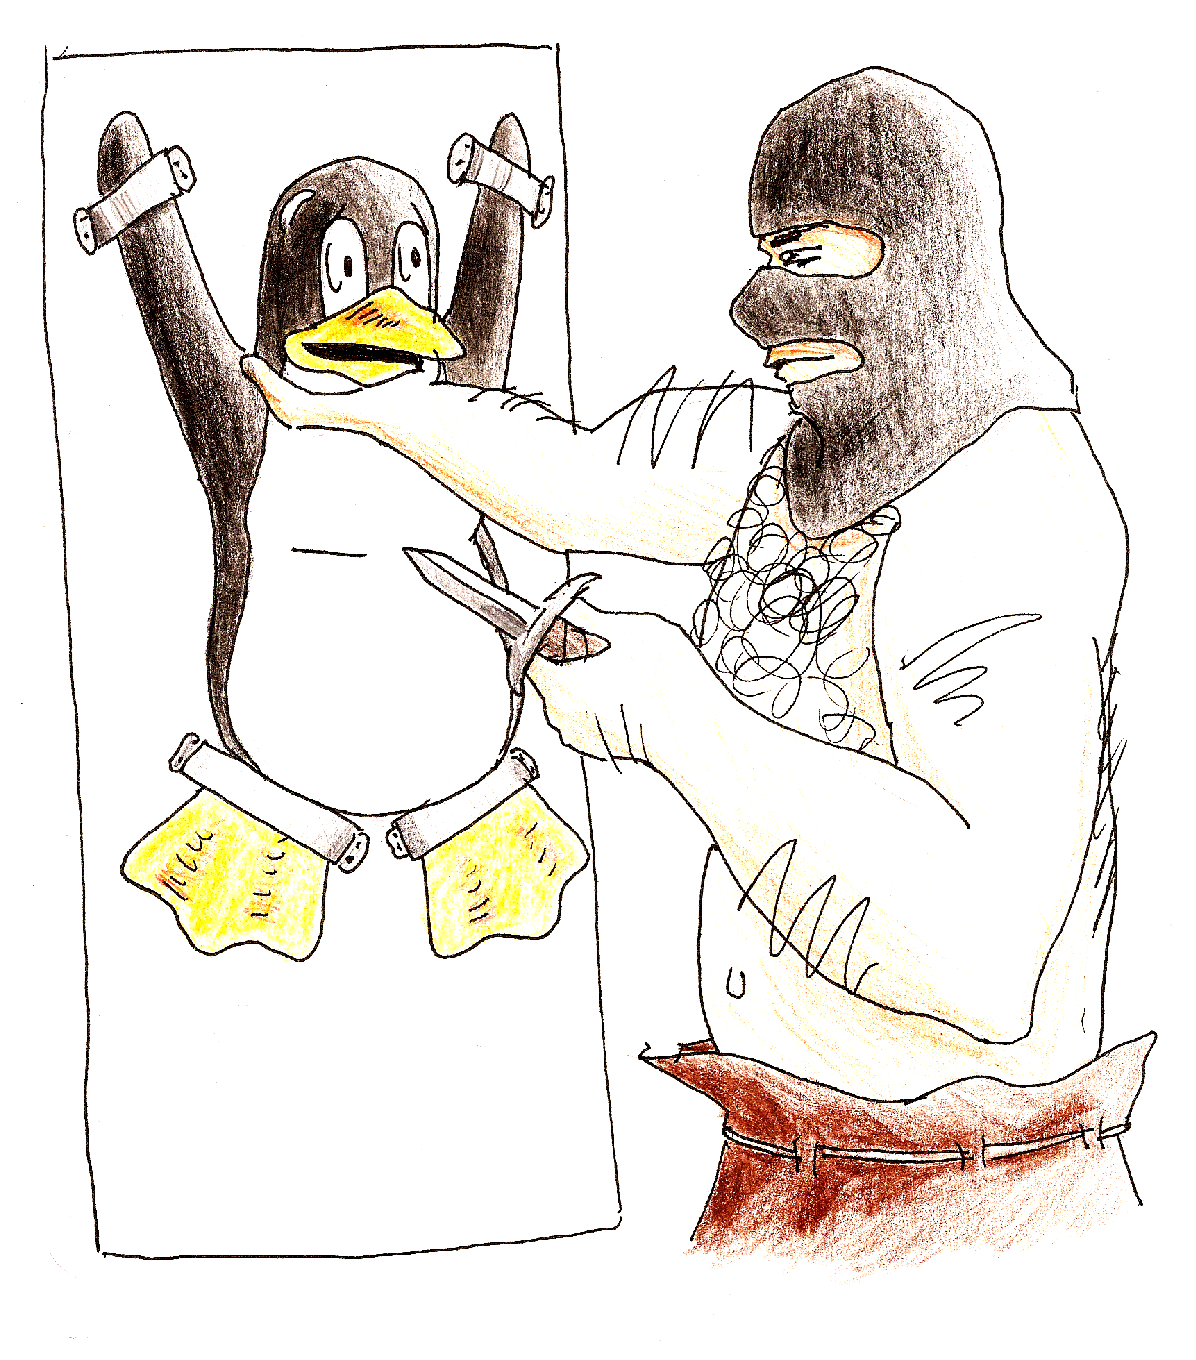
\includegraphics{cartoons/TortureTux}}
\caption{Validation and the Geneva Convention}
\ContributedBy{Figure}{fig:debugging:Validation and the Geneva Convention}{Melissa Broussard}
\end{figure}

\begin{figure}[tb]
\centering
\resizebox{2in}{!}{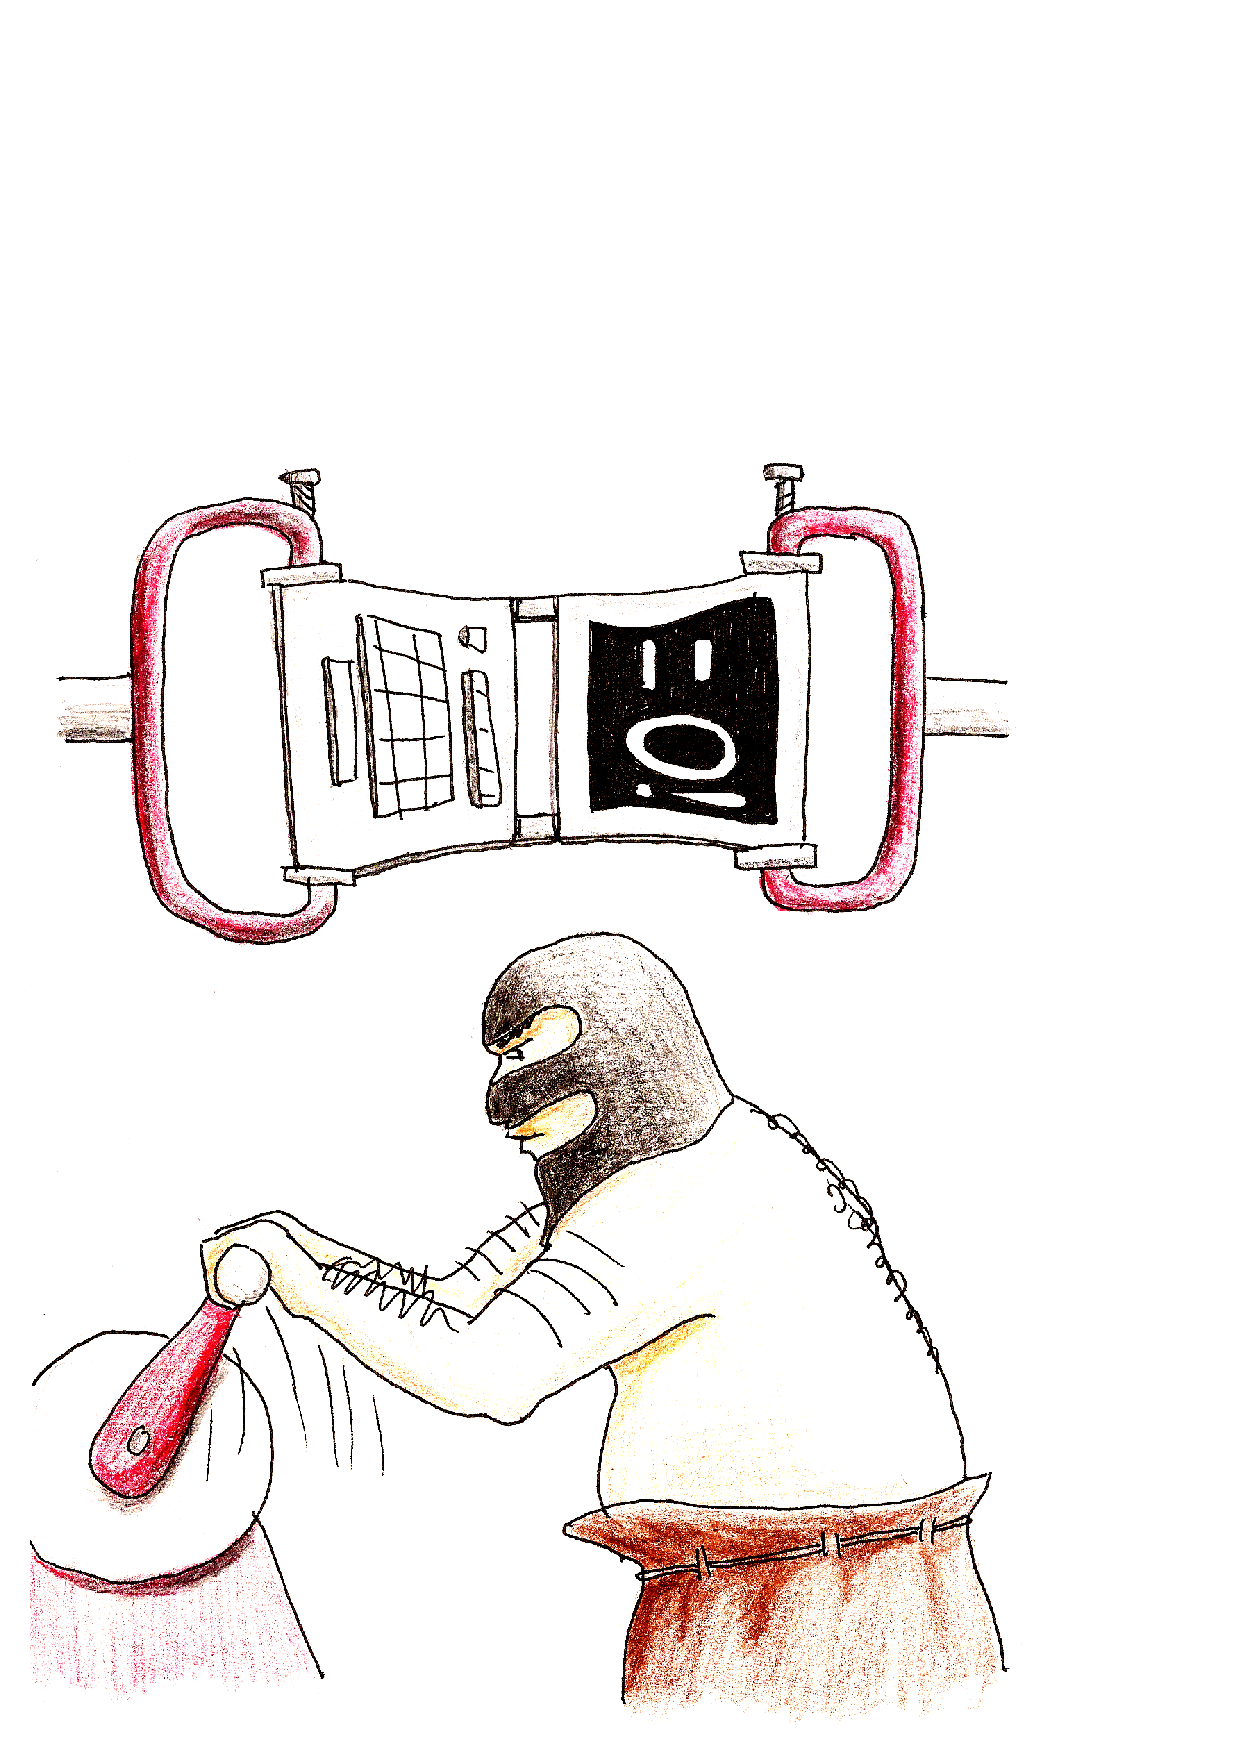
\includegraphics{cartoons/TortureLaptop}}
\caption{Rationalizing Validation}
\ContributedBy{Figure}{fig:debugging:Rationalizing Validation}{Melissa Broussard}
\end{figure}

어떤 사람들에게 격렬한 검증은
Figure~\ref{fig:debugging:Validation and the Geneva Convention} 에 보여진 것
같은 고문의 형태로 보여질 수도 있습니다.\footnote{
	더 시니컬한 사람은 이런 사람들이 단순히 그 검증을 통해 그들이 고쳐야 할
	버그를 찾는 것을 걱정하는 것 뿐 아니냐는 질문을 할수도 있겠죠.}
그런 사람들은
Figure~\ref{fig:debugging:Rationalizing Validation} 에 그려진 것처럼 Tux 그림과
달리, 실제로는 애니메이션이 아닌 물건들을 고문하고 있음을 마음에 되새기는게
도움이 될겁니다.

하지만, 이러고 마는건 프로젝트의 진행 과정 중 정확히 언제 검증이 시작되어야
하는지에 대한 의문을 남겨두게 되는데, 이 주제는 다음 섹션에서 다루어집니다.
\iffalse

Some people might see vigorous validation as a form of torture, as
depicted in
Figure~\ref{fig:debugging:Validation and the Geneva Convention}.\footnote{
	More cynical people might question whether these people are instead
	merely afraid that validation will find bugs that they will then
	be expected to fix.}
Such people might do well to remind themselves that, Tux cartoons aside,
they are really torturing an inanimate object, as shown in
Figure~\ref{fig:debugging:Rationalizing Validation}.
In addition, rest assured that those who fail to torture their code are
doomed to be tortured by it.

However, this leaves open the question of exactly when during the project
lifetime validation should start, a topic taken up by the next section.
\fi

\subsection{When Should Validation Start?}
\label{sec:debugging:When Should Validation Start?}

검증은 프로젝트가 시작된 것과 같은 시점에서부터 시작되어야 합니다.

이 점을 알기 위해, 버그를 추적하는 것은 작은 프로그램에서보다 큰 프로그램에서
훨씬 더 어렵단 점을 생각해 보세요.
따라서, 버그들을 추적하는데 필요한 시간과 노력을 최소화하기 위해서, 코드의 작은
단위들을 테스트 해야 합니다.
모든 버그들을 이런 방식으로 찾지는 않겠지만, 상당한 양을 이렇게 찾을 것이고,
이런 방식으로 버그들을 찾아내고 찾아낸 버그들을 고치는게 훨씬 더 쉬울 겁니다.
이 수준에서의 테스트는 전체 설계에 있는 더 커다란 결점을 알릴 수도 있어서,
설계로 인해 문자 그대로 상당히 고장나 있는 코드를 쓰느라 낭비하는 시간을 최소화
시켜줄 겁니다.
\iffalse

Validation should start at the same time that the project starts.

To see this, consider that tracking down a bug is much harder in a large
program than in a small one.
Therefore, to minimize the time and effort required to track down bugs,
you should test small units of code.
Although you won't find all the bugs this way, you will find a substantial
fraction, and it will be much easier to find and fix the ones you do find.
Testing at this level can also alert you to larger flaws in your overall
design, minimizing the time you waste writing code that is quite literally
broken by design.
\fi

하지만 당신의 설계를 검증하기 전에 왜 코드가 만들어지기를 기다려야
할까요?\footnote{
	``일단 코드를 짜야 하고, 그러고 나면 생각을 할 수 있다는 보상을
	얻는다''는 오래된 말은 통하지 않습니다.}
Chapter~\ref{chp:Hardware and its Habits}
와~\ref{chp:Tools of the Trade} 를 읽으면 일부 유감스럽게도 흔한 설계상의
잘못들을 피하는데 필요한 정보들을 얻을 수 있을 겁니다만, 당신의 설계를 동료와
토론하거나 심지어 단순히 그걸 글자로 써보는 것만으로도 추가적인 결함을 찾아낼
수 있을 겁니다.
\iffalse

But why wait until you have code before validating your design?\footnote{
	The old saying ``First we must code, then we have incentive to
	think'' notwithstanding.}
Hopefully reading Chapters~\ref{chp:Hardware and its Habits}
and~\ref{chp:Tools of the Trade} provided you with the information
required to avoid some regrettably common design flaws,
but discussing your design with a colleague or even simply writing it
down can help flush out additional flaws.
\fi

하지만, 설계를 마칠 때까지 검증의 시작을 기다리는 것은 너무나도 대부분의 경우
너무 오래 기다리고 있는 것입니다.
당신의 자연적인 수준의 낙관은 당신이 요구사항들을 완전히 이해하기 전에 설계를
시작하도록 하는 일은 없었을까요?
이 질문에 대한 대답은 거의 항상 ``그렇다'' 입니다.
잘못된 요구사항을 막는 한가지 좋은 방법은 당신의 사용자들에 대해서 아는
것입니다.
정말로 그들을 위해 봉사를 잘 하려 한다면, 그들과 함께 살아야만 합니다.
\iffalse

However, it is all too often the case that waiting to start validation
until you have a design is waiting too long.
Mightn't your natural level of optimism caused you to start the design
before you fully understood the requirements?
The answer to this question will almost always be ``yes''.
One good way to avoid flawed requirements is to get to know your users.
To really serve them well, you will have to live among them.
\fi

\QuickQuiz{}
	지금 저에게 코딩을 시작하기도 전에 검증을 시작하라고 말씀하시는
	거예요???
	그건 마치 아무것도 시작하지 않는 훌륭한 방법처럼 들리네요!!!
	\iffalse

	You are asking me to do all this validation BS before
	I even start coding???
	That sounds like a great way to never get started!!!
	\fi
\QuickQuizAnswer{
	그게 당신의 프로젝트라면, 예를 들어 취미라면, 원하는 대로 하세요.
	당신이 낭비하는 모든 시간은 당신만의 것이고, 그걸 신경쓸 어떤 사람도
	존재하지 않습니다.
	그리고 시간이 전혀 낭비되지 않을 수 있는 좋은 기회도 있지요.
	예를 들어, 당신이 세상에 없던 최초의 종류의 프로젝트에 착수했다면,
	요구사항들은 어떤 방법으로도 알 수 없는 것들일 겁니다.
	이 경우, 최선의 방법은 빠르게 여러개의 대략적 해결책의 프로토타입들을
	만들어 보고, 그걸 사용해 보고, 뭐가 가장 잘 동작하는지 보는 겁니다.

	다른 한편으로, 당신이 이미 존재하는 시스템과 전체적으로 유사한 시스템을
	만들도록 돈을 받았다면, 당신은 당신의 사용자인 고용인에게 빚을 지고
	있는 것이고 당신의 미래는 빨리 그리고 자주 검증해야 하는 것입니다.
	\iffalse

	If it is your project, for example, a hobby, do what you like.
	Any time you waste will be your own, and you have no one else
	to answer to for it.
	And there is a good chance that the time will not be completely
	wasted.
	For example, if you are embarking on a first-of-a-kind project,
	the requirements are in some sense unknowable anyway.
	In this case, the best approach might be to quickly prototype
	a number of rough solutions, try them out, and see what works
	best.

	On the other hand, if you are being paid to produce a system that
	is broadly similar to existing systems, you owe it to your users,
	your employer, and your future self to validate early and often.
	\fi
} \QuickQuizEnd

세상에 없던 새로운 종류의 프로젝트들은 검증에 있어 다른 전략을 필요로 하는데,
예를 들면, 빠른 프로토타입 만들기 입니다.
여기서, 처음의 몇개 프로토타입들의 목표는 이 프로젝트가 어떻게 구현되는지를
배우는 것이지, 처음부터 올바른 구현을 만드는게 아닙니다.
하지만, 근본적으로 다른 전략을 취하기보다는, 검증을 누락시켜선 안된다는 것을
명심하는게 중요합니다.

이제 우리는 당신이 프로젝트를 시작할 때부터 검증을 시작해야 하는걸로
합의했으니, 다음 섹션들에서는 그 가치가 이미 증명된 여러가지 검증 기술들과
방법들을 알아보겠습니다.
\iffalse

First-of-a-kind projects
require different approaches to validation, for example,
rapid prototyping.
Here, the main goal of the first few prototypes is to learn how
the project should be implemented, not so much to create a correct
implementation on the first try.
However, it is important to keep in mind that you should not omit
validation, but rather take a radically different approach to it.

Now that we have established that you should start validation when you
start the project, the following sections cover a number of validation
techniques and methods that have proven their worth.
\fi

\subsection{The Open Source Way}
\label{sec:debugging:The Open Source Way}

오픈소스 프로그래밍 방법론은 상당히 효율적임이 증명되었고, 격렬한 코드 리뷰와
테스트 제도를 포함하고 있습니다.

전 개인적으로 오픈소스 커뮤니티의 격렬한 코드리뷰의 효율성을 증명할 수
있습니다.
제가 리눅스 커널을 위해 준비했던 첫번째 패치들은 분산 파일시스템에 관한
것이었는데, 이 파일시스템에서 한 노드의 사용자는 다른 노드의 사용자가 메모리에
매핑해둔 파일의 한 지역에 쓰기를 할 수 있었습니다.
이 경우, 이 파일시스템이 쓰기 작업 중에도 일관성을 유지할 수 있도록 하기 위해,
관련된 페이지들을 해당 매핑으로부터 무효화 시킬 필요가 있습니다.
저는 첫번째 시도를 패치로 코딩했고, 오픈 소스의 ``빨리 공유하고, 자주 공유할
것'' 이라는 행동 원리를 명심하고 있었기에, 그 패치를 공유했습니다.
그러고나서 저는 제가 그걸 어떻게 테스트해야 하나 고민했습니다.
\iffalse

The open-source programming methodology has proven quite effective, and
includes a regimen of intense code review and testing.

I can personally attest to the effectiveness of the open-source community's
intense code review.
One of the first patches I prepared for the Linux kernel involved
a distributed filesystem where a user on one node writes to a given
file at a location that a user on another node has mapped into memory.
In this case, it is necessary to invalidate the affected pages from
the mapping in order to allow the filesystem to maintain coherence
during the write operation.
I coded up a first attempt at a patch, and, in keeping with the open-source
maxim ``post early, post often'', I posted the patch.
I then considered how I was going to test it.
\fi

하지만 제가 전체적인 테스트 전략을 결정하기도 전에 저는 제가 공유한 내용에 대해
몇개의 버그를 지적하는 답변을 받았습니다.
전 그 버그들을 고쳐서 패치를 다시 공유했고, 다시 제 테스트 전략에 대해 생각하는
단계로 돌아왔습니다.
하지만, 제가 테스트 코드를 작성할 시간을 갖기도 전에, 저는 더 많은 버그들을
지적하는, 제가 재공유한 패치에 대한 답변을 받았습니다.
이 프로세스는 그 자체로 여러번 반복되었고, 전 제가 그 패치를 정말로 테스트할
기회를 갖기는 했었는지 확신하지 못하겠습니다.
\iffalse

But before I could even decide on an overall test strategy, I got a
reply to my posting pointing out a few bugs.
I fixed the bugs and reposted the patch, and returned to thinking
out my test strategy.
However, before I had a chance to write any test code, I received
a reply to my reposted patch, pointing out more bugs.
This process repeated itself many times, and I am not sure that I
ever got a chance to actually test the patch.
\fi

이 경험은 오픈소스가 정말로 말하는 것이 무엇인지 알려줬습니다:
충분한 눈이 있다면, 모든 버그들은 쉽게 파악될 수 있다~\cite{EricSRaymond99b}.

하지만, 당신이 어떤 코드나 패치를 공유하려 한다면, 몇가지 질문을 해보는게 좋을
겁니다:
\iffalse

This experience brought home the truth of the open-source saying:
Given enough eyeballs, all bugs are shallow~\cite{EricSRaymond99b}.

However, when you post some code or a given patch, it is worth
asking a few questions:
\fi

\begin{enumerate}
\item	얼마나 많은 눈이 당신의 코드를 정말로 보게 될까요?
\item	얼마나 많은 눈이 당신의 버그를 정말로 찾기에 충분할 정도로 경험이 많고
	현명할까요?
\item	정확히 언제 그들이 당신의 코드를 볼까요?
\iffalse

\item	How many of those eyeballs are actually going to look at your code?
\item	How many will be experienced and clever enough to actually find
	your bugs?
\item	Exactly when are they going to look?
\fi
\end{enumerate}

전 운이 좋았습니다:  제 패치로 제공되는 기능을 필요로 하는 누군가가 거기에
있었는데, 그는 분산 파일시스템들에 긴 경험을 가지고 있었고, 제 페치를 거의
곧바로 보았습니다.
아무도 제 패치를 보지 않았다면, 어떤 리뷰도 없었을 것이고, 따라서 버그를 찾지도
못했을 겁니다.
만약 제 패치를 보는 사람들이 분산 파일시스템들에 대한 경험이 부족했다면, 그들이
모든 버그들을 찾지는 못했을 겁니다.
그들이 코드를 보기 전에 몇달이나 심지어 몇년간을 기다려야 했다면, 전 그 패치가
어떻게 동작해야 했는지도 잊어버려서 그 버그들을 고치기도 훨씬 더 어려웠을
겁니다.
\iffalse

I was lucky:  There was someone out there who wanted the functionality
provided by my patch, who had long experience with distributed filesystems,
and who looked at my patch almost immediately.
If no one had looked at my patch, there would have been no review, and
therefore no finding of bugs.
If the people looking at my patch had lacked experience with distributed
filesystems, it is unlikely that they would have found all the bugs.
Had they waited months or even years to look, I likely would have forgotten
how the patch was supposed to work, making it much more difficult to
fix them.
\fi

하지만, 우린 오픈소스 개발의 두번째 교리인 격렬한 테스트를 잊지 말아야만
합니다.
예를 들어, 엄청나게 많은 사람들이 리눅스 커널을 테스트 합니다.
어떤 사람들은 패치들을 제출되자마자 테스트하는데, 당신의 것도 그 대상이 될 수
있습니다.
어떤 사람들은 -next 트리를 테스트하는데, 이는 도움이 되지만, 당신이 패치를
작성한 시점부터 그게 -next 트리에 들어가게 되는 시점까지는 몇주에서 몇달까지의
지연이 있을 수도 있는데, 이는 그 패치가 당신의 기억 속에 여전히 아주 생생하게
남아있지는 않을 가능성이 있는 시간입니다.
어떤 사람들은 메인테이너 트리들을 테스트 하는데, 이때에도 비슷한 지연시간이
있곤 합니다.
\iffalse

However, we must not forget the second tenet of the open-source development,
namely intensive testing.
For example, a great many people test the Linux kernel.
Some test patches as they are submitted, perhaps even yours.
Others test the -next tree, which is helpful, but there is likely to be
several weeks or even months delay between the time that you write the
patch and the time that it appears in the -next tree, by which time the
patch will not be quite as fresh in your mind.
Still others test maintainer trees, which often have a similar time delay.
\fi

일부 적은 사람들은 메인라인 또는 마스터 소스 트리 (리눅스 커널의 경우라면 Linus
의 트리) 에 커밋되기 전까지는 코드를 테스트 하지 않습니다.
당신의 메인테이너가 테스트 되기 전까지는 당신의 패치를 받아주지 않는다면, 이는
당신에게 데드락 상황을 보이게 합니다: 당신의 패치는 테스트 되기 전까지는
받아들여지지 않을텐데, 이 패치는 또한 받아들여지기 전까지는 테스트 되지 않을
겁니다.
더도 아니고 덜도 아니고, 많은 사람들과 단체들이 코드가 리눅스 배포판에 들어가기
전까지는 그 코드를 테스트 하지 않기 때문에, 메인라인 코드를 테스트하는 사람들은
여전히 상대적으로 공격적입니다.
\iffalse

Quite a few people don't test code until it is committed to mainline,
or the master source tree (Linus's tree in the case of the Linux kernel).
If your maintainer won't accept your patch until it has been tested,
this presents you with a deadlock situation: your patch won't be accepted
until it is tested, but it won't be tested until it is accepted.
Nevertheless, people who test mainline code are still relatively
aggressive, given that many people and organizations do not test code
until it has been pulled into a Linux distro.
\fi

그리고 누군가가 당신의 패치를 테스트 한다고 하더라도, 그들이 당신의 버그들을
찾아내는데 필요한 하드웨어와 소프트웨어 구성과 워크로드를 수행할것인지에
대해서는 보장이 없습니다.

따라서, 오픈소스 프로젝트를 위한 코드를 작성할 때라 할지라도, 당신은 당신
스스로의 테스트 장비를 개발하고 수행할 준비를 할 필요가 있습니다.
테스트 개발은 실제 가치에 비해 덜 중요하게 평가되었지만 매우 중요한 기술이므로,
당신이 사용할 수 있는, 이미 존재하는 테스트 장비들의 장점을 모두 취할 수 있도록
하십시오.
테스트 개발이 그렇게 중요하므로, 우리는 그에 대한 더이상의 토론은 그 주제
전용의 책들에게 떠넘기도록 하겠습니다.
따라서 다음의 섹션들은 당신이 이미 좋은 테스트 장비를 갖추고 있다는 가정 하에
당신의 코드 안의 버그들을 찾는 방법들을 다루겠습니다.
\iffalse

And even if someone does test your patch, there is no guarantee that they
will be running the hardware and software configuration and workload
required to locate your bugs.

Therefore, even when writing code for an open-source project, you need to
be prepared to develop and run your own test suite.
Test development is an underappreciated and very valuable skill, so be
sure to take full advantage of any existing test suites available to
you.
Important as test development is, we will leave further discussion of it
to books dedicated to that topic.
The following sections therefore discuss locating bugs in your code given that
you already have a good test suite.
\fi

\section{Tracing}
\label{sec:debugging:Tracing}
%
\epigraph{The machine knows what is wrong.  Make it tell you.}{\emph{Unknown}}

다른 모든게 실패한다면, \co{printk()} 를 추가하세요!
또는, 사용자 모드 C-언어 어플리케이션을 작업 중이라면 \co{printf()} 를요.

논리적 근거는 간단합니다: 어떻게 실행이 코드의 특정 지점까지 가게 되었는지
알아낼 수가 없다면, 무슨 일이 벌어졌는지 알아내기 위해 코드의 앞부분에
프린트문을 여기저기 집어넣으세요.
비슷한 효과를 (유저 어플리케이션을 위한) gdb 나 (리눅스 커널 디버깅을 위한)
kgdb 와 같은 디버거를 이용해서 더 편리하고 유연성 있게 얻을 수도 있습니다.
훨씬 더 세련된 도구들도 존재하는데, 그 중 최신의 일부는 문제가 발생한 시점부터
뒤로 시간을 되돌릴 수 있는 기능을 제공합니다.
\iffalse

When all else fails, add a \co{printk()}!
Or a \co{printf()}, if you are working with user-mode C-language applications.

The rationale is simple: If you cannot figure out how execution reached
a given point in the code, sprinkle print statements earlier in the
code to work out what happened.
You can get a similar effect, and with more convenience and flexibility,
by using a debugger such as gdb (for user applications) or kgdb
(for debugging Linux kernels).
Much more sophisticated tools exist, with some of the more recent
offering the ability to rewind backwards in time from the point
of failure.
\fi

이런 간단한 테스트 도구들은 모두 가치가 있는데, 일반적인 시스템들이 64K 보다 큰
메모리와 4MHz 보다 빠른 속도로 동작하는 지금에 있어선 특히 그렇습니다.
이런 도구들에 대해서는 더 많은 글들이 있으므로, 이 챕터는 그에 대해 조금만 더
이야기 하겠습니다.
\iffalse

These brute-force testing tools are all valuable, especially now
that typical systems have more than 64K of memory and CPUs running
faster than 4\,MHz.
Much has been
written about these tools, so this chapter will add little more.
\fi

하지만, 이런 도구들은 모두, 디버깅하려는 일이 고성능의 병렬 알고리즘의 빠른
수행경로에 뭐가 잘못되어 있는지를 알려고 하는 것일 경우에 심각한 단점을 가지고
있는데, 달리 말해 대부분의 경우 큰 오버헤드를 갖습니다.
이런 목적을 위한 특수한 추적 기술들이 있는데, 일반적으로 실행시간 데이터 수집의
오버헤드를 최소화 하기 위해 데이터 소유권 테크닉
(Chapter~\ref{chp:Data Ownership}을 참고하세요) 을 사용합니다.
리눅스 커널에서의 한가지 예는 데이터가 극단적으로 낮은 오버헤드만을 가지고
수집될 수 있도록 하기 위해 CPU 별 버퍼를 사용하는
``trace events''~\cite{StevenRostedt2010perfTraceEventP1,StevenRostedt2010perfTraceEventP2,StevenRostedt2010perfTraceEventP3,StevenRostedt2010perfHP+DeathlyMacros}
입니다.
그렇다 하더라도, 추적 기능을 활성화 시키는 것은 어떤 경우에는 버그를 숨기기
충분할 만큼 타이밍을 바꿀 수 있어서,
Section~\ref{sec:debugging:Probability and Heisenbugs} 과
Section~\ref{sec:debugging:Hunting Heisenbugs} 에서 특별히 다루어질
\emph{heisenbugs} 를 초래할 수 있습니다.
\iffalse

However, these tools all have a serious shortcoming when the job at hand
is to convince a the fastpath of a high-performance parallel algorithm
to tell you what is going wrong, namely, they often have excessive
overheads.
There are special tracing technologies for this purpose, which typically
leverage data ownership techniques
(see Chapter~\ref{chp:Data Ownership})
to minimize the overhead of runtime data collection.
One example within the Linux kernel is
``trace events''~\cite{StevenRostedt2010perfTraceEventP1,StevenRostedt2010perfTraceEventP2,StevenRostedt2010perfTraceEventP3,StevenRostedt2010perfHP+DeathlyMacros},
which uses per-CPU buffers to allow data to be collected with
extremely low overhead.
Even so, enabling tracing can sometimes change timing enough to
hide bugs, resulting in \emph{heisenbugs}, which are discussed in
Section~\ref{sec:debugging:Probability and Heisenbugs}
and especially Section~\ref{sec:debugging:Hunting Heisenbugs}.
\fi

유저스페이스 코드에는, 여러분을 도울 수많은 도구들이 있습니다.
이를 알아보는데 있어 시작하기 좋은 것은 Brendan Gregg 의
블로그입니다.\footnote{
	\url{http://www.brendangregg.com/blog/}}

Heisenbug 를 막는다 하더라도, 다른 위험들이 기다리고 있습니다.
예를 들어, 비록 기계는 모든 것을 알고 있지만, 그것이 알고 있는 것은 거의 항상
당신의 머리가 쥐고 있을 수 있는 것보다 많은 정보입니다.
이런 이유로, 높은 품질의 테스트 장비들은 일반적으로 대량의 출력을 분석할 수
있도록 세련된 스크립트들을 함께 제공합니다.
하지만 조심하세요---스크립트들은 놀라운 일을 알려줘야만 하는 건 아닙니다.
제 rcutorture 스크립트는 그런 점에서의 한 경우입니다: 그 스크립트들의 초기
버전들은 RCU grace period 들이 불명확하게 늦춰지며 동작 (stall) 함에도 문제가
없다고 판단하고는 했습니다.
이는 물론 해당 스크립트들이 RCU grace-period stall 문제를 파악할 수 있도록
수정되었습니다만, 이로 인해 해당 스크립트는 제가 파악할 수 있게 하자고 생각하는
문제들만을 파악한다는 사실은 바뀌지 않습니다.
그 스크립트들은 유용합니다만, 가끔 rcutorture 출력을 일일이 읽는 행위를 대체할
수는 없습니다.
하지만 여러분이 훌륭한 설계를 갖지 않는다면, 여러분은 여러분의 스크립트가
무엇을 체크해야 하는지도 모를 수 있음을 알아두시기 바랍니다!
\iffalse

In userspace code, there is a huge number of tools that can help you.
One good starting point is Brendan Gregg's blog.\footnote{
	\url{http://www.brendangregg.com/blog/}}

Even if you avoid heisenbugs, other pitfalls await you.
For example, although the machine really does know all,
what it knows is almost always way more than your head can hold.
For this reason, high-quality test suites normally come with sophisticated
scripts to analyze the voluminous output.
But beware---scripts won't necessarily notice surprising things.
My rcutorture scripts are a case in point: Early versions of those
scripts were quite satisfied with a test run in which RCU grace periods
stalled indefinitely.
This of course resulted in the scripts being modified to detect RCU
grace-period stalls, but this does not change the fact that the scripts
will only detects problems that I think to make them detect.
But note well that unless you have a solid design, you won't know what
your script should check for!
\fi

추적 기능과 특히 \co{printk()} 호출에 있어서의 또다른 문제는 그 오버헤드가
제품에 사용되기에는 너무 크다는 것입니다.
그런 경우들 중 일부에 있어서는, 단정문들이 도움이 될 수 있습니다.
\iffalse

Another problem with tracing and especially with \co{printk()} calls
is that their overhead is often too much for production use.
In some such cases, assertions can be helpful.
\fi

\section{Assertions}
\label{sec:debugging:Assertions}
%
\epigraph{No man really becomes a fool until he stops asking questions.}
	 {\emph{Charles P. Steinmetz}}

단정문들은 일반적으로 다음과 같은 식으로 구현됩니다:
\iffalse

Assertions are usually implemented in the following manner:
\fi

\vspace{5pt}
\begin{minipage}[t]{\columnwidth}
\tt
\scriptsize
\begin{verbatim}
  1 if (something_bad_is_happening())
  2   complain();
\end{verbatim}
\end{minipage}
\vspace{5pt}

이 패턴은 종종 C 전처리기 매크로나 프로그래밍 언어의 내재 기능으로 캡슐화
되어지는데, 예를 들어 리눅스 커널의 경우, 이는
\co{WARN_ON(something_bad_is_happening())} 으로 표현될 겁니다.
물론, 만약 \co{something_bad_is_happening()} 이 상당히 자주 벌어진다면 그로
말미암은 출력은 다른 문제들의 보고를 이해하기 어렵게 만들 수 있는데, 이런
경우에는 \co{WARN_ON_ONCE(something_bad_is_happening()} 이 더 적절할 겁니다.
\iffalse

This pattern is often encapsulated into C-preprocessor macros or
language intrinsics, for example, in the Linux kernel, this might
be represented as \co{WARN_ON(something_bad_is_happening())}.
Of course, if \co{something_bad_is_happening()} quite frequently,
the resulting output might obscure reports of other problems,
in which case
\co{WARN_ON_ONCE(something_bad_is_happening())} might be more appropriate.
\fi

\QuickQuiz{}
	\co{WARN_ON_ONCE()} 는 어떻게 구현할 수 있을까요?
	\iffalse

	How can you implement \co{WARN_ON_ONCE()}?
	\fi
\QuickQuizAnswer{
	가끔은 두번이나 세번까지는 경고를 날릴 수 있는 \co{WARN_ON_ONCE()} 여도
	문제가 없다면, 간단히 초기값 0을 갖는 static 변수를 사용하세요.
	조건이 만족된다면, 이 static 변수를 체크하고, 만약 0이 아니라면, 그냥
	리턴합니다.
	그렇지 않다면, 그 값을 1으로 설정하고, 메세지를 출력한 후, 리턴하세요.

	경고 메세지가 굉장히 커다랗거나 해서 메세지가 절대로 두번 이상 나타나선
	안된다면 앞의 ``그 값을 1로 설정'' 부분을 어토믹 교환 오퍼레이션을
	사용할 수 있습니다.
	경고 메세지는 이 어토믹 교환 오퍼레이션이 0을 리턴한 경우에만 프린트
	하도록 합니다.
	\iffalse

	If you don't mind having a \co{WARN_ON_ONCE()} that
	will sometimes warn twice or three times, simply maintain
	a static variable that is initialized to zero.
	If the condition triggers, check the static variable, and
	if it is non-zero, return.
	Otherwise, set it to one, print the message, and return.

	If you really need the message to never appear more than once,
	perhaps because it is huge, you can use an atomic exchange
	operation in place of ``set it to one'' above.
	Print the message only if the atomic exchange operation returns
	zero.
	\fi
} \QuickQuizEnd

병렬 코드에서, 일어날 수도 있는 한가지 매우 나쁜 일은 특정한 락이 잡힌 상태에서
호출될 것으로 기대되는 어떤 함수가 그 락이 잡히지 않은 채로 호출되는
경우입니다.
그런 함수들은 어떤 경우에는 ``호출자는 반드시 이 함수를 호출할 때 \co{foo_lock}
을 잡아야만 함''과 같은 이야기를 하는 헤더 코멘트를 가질 수도 있습니다만, 그런
코멘트는 누군가가 그걸 정말로 읽지 않는다면 어떤 좋은 일도 하지 않습니다.
\co{lock_is_held(&foo_lock)} 과 같이 실행 가능한 이야기가 훨씬 많은 무게를
갖습니다.
\iffalse

In parallel code, one especially bad something that might happen is that
a function expecting to be called under a particular lock might be called
without that lock being held.
Such functions sometimes have header comments stating something like
``The caller must hold \co{foo_lock} when calling this function'', but
such a comment does no good unless someone actually reads it.
An executable statement like \co{lock_is_held(&foo_lock)} carries far
more weight.
\fi

리눅스 커널의 lockdep
기능~\cite{JonathanCorbet2006lockdep,StevenRostedt2011locdepCryptic} 은 이
과정을 좀 더 크게 취하는데, 잠재적인 데드락을 보고하는 것 뿐만 아니라 함수들이
올바른 락들을 잡았는지 검증할 수 있게 도와줍니다.
물론, 이 추가적인 기능은 상당한 오버헤드를 만들어내는데, 그로인해 lockdep 은
제품에서의 사용에는 적합하지는 않습니다.

그래서 검사가 필요하지만 실행시간에서의 검사로 인한 오버헤드는 용인될 수 없는
경우들에는 무엇을 해볼 수 있을까요?
한가지 방법은 정적 분석인데, 다음 섹션에서 이에 대해 논해 보겠습니다.
\iffalse

The Linux kernel's lockdep
facility~\cite{JonathanCorbet2006lockdep,StevenRostedt2011locdepCryptic}
takes this a step farther, reporting potential deadlocks as well as
allowing functions to verify that the proper locks are held.
Of course, this additional functionality incurs significant overhead,
so that lockdep is not necessarily appropriate for production use.

So what can be done in cases where checking is necessary, but where the
overhead of runtime checking cannot be tolerated?
One approach is static analysis, which is discussed in the next section.
\fi

\section{Static Analysis}
\label{sec:debugging:Static Analysis}
%
\epigraph{A lot of automation isn't a replacement of
	  humans but of mind-numbing behavior.}
	 {\emph{Summarized from Stewart Butterfield}}

정적 분석인 첫번째 프로그램이 두번째 프로그램을 입력으로 받아서 두번째 프로그램
안에 있는 에러들과 취약점들을 보고해 주는 검증 테크닉입니다.
흥미롭게도, 거의 모든 프로그램들이 컴파일러와 인터프리터들을 통해 정적 분석을
합니다.
이런 도구들은 물론 완벽과는 거리가 멉니다만, 그것들의 에러를 찾아내는 기능은
과거의 수십년간 몹시 개선되었는데, 일부분은 그 분석을 진행할 메모리의 크기가
64K 바이트보다 훨씬 더 커진 것도 한 이유입니다.
\iffalse

Static analysis is a validation technique were one program takes a second
program as input, reporting errors and vulnerabilities located in this
second program.
Interestingly enough, almost all programs are subjected to static analysis
by their compilers or interpreters.
These tools are of course far from perfect, but their ability to locate
errors has improved immensely over the past few decades, in part because
they now have much more than 64K bytes of memory in which to carry out their
analysis.
\fi

원래의 UNIX \co{lint} 도구~\cite{StephenJohnson1977lint} 는 상당히
유용합니다만, 그것의 기능들 가운데 대부분의 것들은 C 컴파일러 안에
포함되었습니다.
더도 아니고 덜도 아니고 lint 와 유사한, 개발되고 있고 사용되고 있는 도구들이
오늘날 존재합니다.

Sparse 정적 분석 도구~\cite{JonathanCorbet2004sparse} 는 리눅스 커널의 높은
수준의 문제들을 찾아내는데, 다음과 같은 문제들을 포함합니다:
\iffalse

The original UNIX \co{lint} tool~\cite{StephenJohnson1977lint} was
quite useful, though much of its functionality has since been incorporated
into C compilers.
There are nevertheless lint-like tools under development and in use to
this day.

The sparse static analyzer~\cite{JonathanCorbet2004sparse}
looks for higher-level issues in the Linux kernel, including:
\fi

\begin{enumerate}
\item	유저 스페이스 구조체로의 포인터의 잘못된 사용.
\item	너무 긴 상수로부터의 값 할당.
\item	텅 빈 \co{switch} 문.
\item	잘못 매치된 락 획득과 해제 도구들.
\item	Per-CPU 도구들의 잘못된 사용.
\item	RCU 포인터가 아닌 곳에서의 RCU 사용과 그 반대 경우.
\iffalse

\item	Misuse of pointers to user-space structures.
\item	Assignments from too-long constants.
\item	Empty \co{switch} statements.
\item	Mismatched lock acquisition and release primitives.
\item	Misuse of per-CPU primitives.
\item	Use of RCU primitives on non-RCU pointers and vice versa.
\fi
\end{enumerate}

컴파일러들이 자체적인 정적 분석 기능들을 계속해서 늘려갈 것 같긴 하지만, sparse
정적 분석 도구는 컴파일러 밖에서의 정적 분석의 효과를 보여주고 있는데, 특히
어플리케이션에 특정한 버그들을 찾는데 그러합니다.
\iffalse

Although it is likely that compilers will continue to increase their
static-analysis capabilities, the sparse static analyzer demonstrates
the benefits of static analysis outside of the compiler, particularly
for finding application-specific bugs.
\fi

\section{Code Review}
\label{sec:debugging:Code Review}
%
\epigraph{If a man speaks of my virtues, he steals from me;
	  if he speaks of my vices, then he is my teacher.}
	 {\emph{Chinese proverb}}

다양한 코드 리뷰 활동들은 정적 분석의 특수한 경우들입니다만, 사람이 분석을
한다는 차이가 있습니다.
이 섹션은 검사, 가상 리허설, 그리고 자가 검사에 대해서 다룹니다.
\iffalse

Various code-review activities are special cases of static analysis, but
with human beings doing the analysis.
This section covers inspection, walkthroughs, and self-inspection.
\fi

\subsection{Inspection}
\label{sec:debugging:Inspection}

전통적으로, 정식적인 코드 검사는 정식적으로 정의된 역할들의 얼굴을 맞대는
모임으로 이루어졌습니다: 중재자, 개발자, 그리고 한두명의 참가자.
여기서 개발자는 코드를 읽어내려가면서 그 코드가 하는 일이 무엇이며 왜
동작하는지 설명을 합니다.
한두명의 참가자들은 질문을 하고 문제를 제기하며, 중재자가 하는 일은 모든 충돌을
처리하고 기록을 하는 것입니다.
이 과정은 버그를 찾아내는 데에 상당히 효과적일 수 있는데, 모든 참가자가 이
코드에 친숙하다면 특히 그러합니다.
\iffalse

Traditionally, formal code inspections take place in face-to-face meetings
with formally defined roles: moderator, developer, and one or two other
participants.
The developer reads through the code, explaining what it is doing and
why it works.
The one or two other participants ask questions and raise issues, while
the moderator's job is to resolve any conflicts and to take notes.
This process can be extremely effective at locating bugs, particularly
if all of the participants are familiar with the code at hand.
\fi

하지만, 이 얼굴을 맞대는 정식적 과정은 글로벌한 리눅스 커널 커뮤니티에서는 잘
동작하지 못할 수 있습니다, IRC 세션을 사용하면 어쩌면 잘 동작할 수도
있겠지만요.
대신에, 개인들은 코드를 개별적으로 리뷰하고 이메일이나 IRC 를 통해 코멘트를
제공합니다.
기록을 하는 행위는 이메일 기록이나 IRC 로그를 통해 제공되며, 중재자들은 그들의
서비스들을 적절하게 자발적으로 봉사합니다.
간헐적인 격론을 주고 받으면서, 이 프로세스는 합리적인 수준으로 잘 동작하는데,
모든 참가자들이 처리해야 하는 코드에 모두 친숙하다면 더욱 그러합니다.\footnote{
	그렇다곤 하나, 전통적인 정식적 검사에 비한 리눅스 커널 커뮤니티 방법의
	장점 가운데 하나는 코드에 친숙하지 \emph{않은}, 따라서 코드에 익숙한
	사람들에게 품어져 있는 옳지 않은 가정에 의해 눈이 가려지지 않은
	사람들의 기여의 가능성이 훨씬 더 높다는 것입니다.}
\iffalse

However, this face-to-face formal procedure does not necessarily
work well in the global Linux kernel community, although it might work
well via an IRC session.
Instead, individuals review code separately and provide comments via
email or IRC.
The note-taking is provided by email archives or IRC logs, and moderators
volunteer their services as appropriate.
Give or take the occasional flamewar, this process also works reasonably
well, particularly if all of the participants are familiar with the
code at hand.\footnote{
	That said, one advantage of the Linux kernel community approach
	over traditional formal inspections is the greater probability of
	contributions from people \emph{not} familiar with the code,
	who therefore might not be blinded by the invalid assumptions
	harbored by those familiar with the code.}
\fi

리눅스 커널 커뮤니티의 리뷰 프로세스는 개선될 여지도 많습니다:
\iffalse

It is quite likely that the Linux kernel community's review process
is ripe for improvement:
\fi

\begin{enumerate}
\item	가끔은 효과적인 리뷰를 하기에 충분한 시간과 전문성을 가진 사람이 부족할
	때가 있습니다.
\item	모든 리뷰 과정의 토론들이 기록된다고는 하지만, 이 기록들은 통찰이
	잊혀지거나 사람들이 그 토론을 열어보는데에 종종 실패하는 것과 같은
	형태로 ``누실'' 되기도 합니다.
\item	가끔은 격렬한 토론으로 인한 싸움이 벌어졌을 때에 이를 해결하기가 어려울
	수도 있는데, 싸우는 사람들이 합치될 수 없는 목표, 경험, 그리고 어휘를
	사용할 때에 특히 그렇습니다.
\iffalse

\item	There is sometimes a shortage of people with the time and
	expertise required to carry out an effective review.
\item	Even though all review discussions are archived, they are
	often ``lost'' in the sense that insights are forgotten and
	people often fail to look up the discussions.
	This can result in re-insertion of the same old bugs.
\item	It is sometimes difficult to resolve flamewars when they do
	break out, especially when the combatants have disjoint
	goals, experience, and vocabulary.
\fi
\end{enumerate}

따라서, 리뷰를 할 때에는 커밋 로그, 버그 레포트, 그리고 LWN 기사에 있는 적절한
문서들을 참고하는게 좋습니다.
\iffalse

When reviewing, therefore, it is worthwhile to review relevant documentation
in commit logs, bug reports, and LWN articles.
\fi

\subsection{Walkthroughs}
\label{sec:debugging:Walkthroughs}

전통적인 walkthrough (가상 리허설) 는 정식적인 검사와 비슷하지만, 사람들이
코드를 가지고 특정 테스트 케이스에 대해서 ``컴퓨터인 척 한다''는 점이 다릅니다.
일반적인 walkthrough 팀은 중재자, 비서 (찾아낸 버그를 기록합니다), 테스트
전문가 (테스트 케이스를 만들어냅니다), 그리고 한두명의 추가적인 사람들을
포함합니다.
이것들은 굉장히 시간을 소모하지만 상당히 효과적일 수 있습니다.
\iffalse

A traditional code walkthrough is similar to a formal inspection,
except that the group
``plays computer'' with the code, driven by specific test cases.
A typical walkthrough team has a moderator, a secretary (who records
bugs found), a testing expert (who generates the test cases) and
perhaps one to two others.
These can be extremely effective, albeit also extremely time-consuming.
\fi

제가 정식적인 walkthrough 에 참여한지 수십년이 되었고, 저는 오늘날의
walkthrough 는 단일단계 디버거들을 사용할 수도 있을 거라고 생각합니다.
어떤 사람은 다음과 같이 특히나 가학적인 과정을 떠올릴 수 있을 겁니다:
\iffalse

It has been some decades since I have participated in a formal
walkthrough, and I suspect that a present-day walkthrough would
use single-stepping debuggers.
One could imagine a particularly sadistic procedure as follows:
\fi

\begin{enumerate}
\item	테스터는 테스트 케이스를 제공합니다.
\item	중재자는 특정된 테스트 케이스를 입력으로 해서 디버거 위에서 코드를
	동작시킵니다.
\item	각각의 명령문이 실행되기 전에, 개발자는 해당 명령문의 결과가 무엇일지를
	예상하고 왜 그 결과가 옳은지를 설명합니다.
\item	만약 결과가 개발자에 의해 예상되었던 것과 다르다면, 이는 잠재적인
	버그의 증거로 택해집니다.
\item	병렬 코드에서는 ``동시성 업자 (concurrency shark)'' 가 어떤 코드가 이
	코드와 동시적으로 실행될 수 있을 것인지, 그리고 왜 그런 동시성이 해롭지
	않은지 질문합니다.
\iffalse

\item	The tester presents the test case.
\item	The moderator starts the code under a debugger, using the
	specified test case as input.
\item	Before each statement is executed, the developer is required
	to predict the outcome of the statement and explain why
	this outcome is correct.
\item	If the outcome differs from that predicted by the developer,
	this is taken as evidence of a potential bug.
\item	In parallel code, a ``concurrency shark'' asks what code
	might execute concurrently with this code, and why such
	concurrency is harmless.
\fi
\end{enumerate}

가학적입니다, 분명히.
효과적일까요?
아마도요.
참가자들이 요구사항, 소프트웨어 도구들, 데이터 구조들, 그리고 알고리즘들에 대해
잘 이해하고 있다면, 그 walkthrough 는 상당히 효과적일 수 있습니다.
만약 그렇지 않다면, walkthrough 는 시간 낭비인 경우가 많습니다.
\iffalse

Sadistic, certainly.
Effective?
Maybe.
If the participants have a good understanding of the requirements,
software tools, data structures, and algorithms, then walkthroughs
can be extremely effective.
If not, walkthroughs are often a waste of time.
\fi

\subsection{Self-Inspection}
\label{sec:debugging:Self-Inspection}

개발자들이 모두 자신의 코드를 검사하는데 그렇게 효과적이지는 않은 게
일반적이지만, 합리적인 대안이 없는 상황들도 많이 존재합니다.
예를 들어, 해당 개발자가 그 코드를 볼 수 있도록 허가된 유일한 사람일 수 있고,
다른 능력 있는 개발자들은 모두 너무 바빠서일수도 있고, 또는 문제의 해당 코드가
충분히 기묘하게 생겨서 프로토타입을 선보이기 전까지는 어떤 사람도 그걸 심각하게
바라보도록 설득할수가 없어서일 수도 있습니다.
이런 경우들에, 다음과 같은 방법은 상당히 도움이 되는데, 특히 복잡한 병렬
코드에서 그렇습니다:
\iffalse

Although developers are usually not all that effective at inspecting
their own code, there are a number of situations where there is no
reasonable alternative.
For example, the developer might be the only person authorized to look
at the code, other qualified developers might all be too busy, or
the code in question might be sufficiently bizarre that the developer
is unable to convince anyone else to take it seriously until after
demonstrating a prototype.
In these cases, the following procedure can be quite helpful,
especially for complex parallel code:
\fi

\begin{enumerate}
\item	요구사항, 데이터 구조를 위한 다이어그램, 그리고 설계 선택 사항들에 대한
	합리적 이유등을 가지고 설계 문서를 작성합니다.
\item	전문가에게 자문을 구하고 필요하다면 설계 문서를 업데이트 합니다.
\item	코드를 종이 위에 펜으로 써가면서 에러들을 고칩니다.
	앞서 존재한 거의 동일한 코드 시퀀스를 참고하려는 유혹을 견뎌내고,
	작성한 코드의 사본을 만듭니다.
\item	거기에 에러가 있었다면, 깨끗한 종이에 그 코드를 똑같이 쓰면서 에러들을
	고쳐갑니다.
	마지막 두 복사본이 동일할 때까지 이를 반복합니다.
\item	모든 분명치 않은 코드에 대해 정확성을 증명합니다.
\item	가능하다면, 코드 조각들을 바닥에서부터 테스트 합니다.
\item	모든 코드가 합쳐지면, 기능성과 스트레스 테스트를 전부 합니다.
\item	코드가 모든 테스트를 통과한다면, 코드 레벨 문서를 작성하는데, 이는 앞서
	이야기한 설계 문서의 확장판이 될수도 있습니다.
\iffalse

\item	Write design document with requirements, diagrams for data structures,
	and rationale for design choices.
\item	Consult with experts, update the design document as needed.
\item	Write the code in pen on paper, correct errors as you go.
	Resist the temptation to refer to pre-existing nearly identical code
	sequences, instead, copy them.
\item	If there were errors, copy the code in pen on fresh paper, correcting
	errors as you go.
	Repeat until the last two copies are identical.
\item	Produce proofs of correctness for any non-obvious code.
\item	Use a source-code control system.
	Commit early; commit often.
\item	Where possible, test the code fragments from the bottom up.
\item	When all the code is integrated (but preferably before),
	do full-up functional and stress testing.
\item	Once the code passes all tests, write code-level documentation,
	perhaps as an extension to the design document discussed above.
	% TODO: Apply
	Fix both the code and the test code as needed.
\fi
\end{enumerate}

제가 새로운 RCU 코드를 위해 성실하게 이 과정을 따라갔을 때, 과정의 마지막에
이르러서는 몇개의 버그들만이 존재했습니다.
몇개의 두드러지는 (그리고 당황스러운) 예외가
있지만~\cite{PaulEMcKenney2011RCU3.0trainwreck}, 전 남들보다 앞서서 이런
버그들을 잡아내고는 합니다.
그렇다고는 하나, 리눅스 커널 사용자의 수와 다양성이 증가함에 따라 이는 점점
어려워지고 있습니다.
\iffalse

When I faithfully follow this procedure for new RCU code, there are
normally only a few bugs left at the end.
With a few prominent (and embarrassing)
exceptions~\cite{PaulEMcKenney2011RCU3.0trainwreck},
I usually manage to locate these bugs before others do.
That said, this is getting more difficult over time as the number and
variety of Linux-kernel users increases.
\fi

\QuickQuiz{}
	어떤 사람이 존재하는 코드를 종이에 펜으로 사본을 만들려 하겠어요???
	그건 그냥 필사 과정에서의 에러의 가능성만 증가시키는 거 아닌가요?
	\iffalse

	Why would anyone bother copying existing code in pen on paper???
	Doesn't that just increase the probability of transcription errors?
	\fi
\QuickQuizAnswer{
	필사 과정에서의 에러가 걱정된다면, 제가 당신에게 \co{diff} 라는 이름의
	정말 멋진 도구를 처음으로 소개해줄 수 있게 해주세요.
	또한, 필사 과정을 진행하는건 상당히 가치있을 수 있습니다:
	\iffalse

	If you are worried about transcription errors, please allow me
	to be the first to introduce you to a really cool tool named
	\co{diff}.
	In addition, carrying out the copying can be quite valuable:
	\fi
	\begin{enumerate}
	\item	많은 코드를 복사하게 된다면 당신은 추상화를 함으로써 얻을 수
		있는 이득을 얻을 수 없을 겁니다.
		코드를 필사하는 행위는 추상화를 위한 커다란 동기 부여를 줄 수
		있습니다.
	\item	코드를 필사하는 행위는 코드가 정말로 새로운 환경에서도 잘
		동작할 것인지 생각해볼 기회를 줍니다.
		인터럽트를 불가능하게 해야 한다거나 어떤 락을 잡아야 한다거나와
		같은, 명확치 않은 제약이 있나요?
	\item	코드를 필사하는 행위는 또한 그 일을 하게 하는데 어떤 더 나은
		방법이 있을지 고민해 볼 시간을 줍니다.
	\iffalse

	\item	If you are copying a lot of code, you are probably failing
		to take advantage of an opportunity for abstraction.
		The act of copying code can provide great motivation
		for abstraction.
	\item	Copying the code gives you an opportunity to think about
		whether the code really works in its new setting.
		Is there some non-obvious constraint, such as the need
		to disable interrupts or to hold some lock?
	\item	Copying the code also gives you time to consider whether
		there is some better way to get the job done.
	\fi
	\end{enumerate}
	그러니까, 그래요, 코드를 필사하세요!
	\iffalse

	So, yes, copy the code!
	\fi
} \QuickQuizEnd

\QuickQuiz{}
	이 과정은 우스꽝스러울 정도로 지나치게 공업화 되어 있어요!
	어떻게 당신은 합리적인 양의 소프트웨어들이 이런 방식으로 작성되었을
	거라고 생각할 수 있는거죠?
	\iffalse

	This procedure is ridiculously over-engineered!
	How can you expect to get a reasonable amount of software
	written doing it this way???
	\fi
\QuickQuizAnswer{
	실제로, 코드를 손으로 복사하는 행위를 반복하는 것은 노동집약적이고 느립니다.
	하지만, 상당한 스트레스 테스트와 정확성 검증과 조합되어진다면, 궁극적인
	성능과 안정성이 필요하고 디버깅이 어려운 복잡한 병렬 코드에 있어서는 이
	또한 상당히 효과적입니다.
	리눅스 커널 RCU 구현이 그런 케이스입니다.
	\iffalse

	Indeed, repeatedly copying code by hand is laborious and slow.
	However, when combined with heavy-duty stress testing and
	proofs of correctness, this approach is also extremely effective
	for complex parallel code where ultimate performance and
	reliability are required and where debugging is difficult.
	The Linux-kernel RCU implementation is a case in point.
	\fi

	한편으로는, 당신이 어떤 데이터를 조작하기 위해 간단한 싱글 쓰레드 셸
	스크립트를 작성하고 있다면, 다른 방법론이 가장 잘 당신을 도와줄 겁니다.
	예를 들어, 당신이 원하는 대로 동작하고 있음을 확신할 수 있도록 하는
	테스트 데이터와 함께 커맨드 하나 하나를 하나씩 대화형 셸에 입력하고,
	그러고 나서 성공한 커맨드들을 스크립트 안에 복사해서 붙여넣을 수 있을
	겁니다.
	마지막으로, 전체 스크립트를 테스트 하세요.
	\iffalse

	On the other hand, if you are writing a simple single-threaded
	shell script to manipulate some data, then you would be
	best-served by a different methodology.
	For example, you might enter each command one at a time
	into an interactive shell with a test data set to make
	sure that it did what you wanted, then copy-and-paste the
	successful commands into your script.
	Finally, test the script as a whole.
	\fi

	도움을 주려 하는 친구나 동료가 있다면, 페어 프로그래밍이 잘 될 수
	있을텐데, 정식적인 디자인 리뷰와 코드리뷰 프로세스에 있어서도
	마찬가지입니다.

	그리고 당신이 취미로 코드를 작성하고 있다면, 뭐가 됐든 하고 싶은대로
	하세요.

	짧게 요약해서, 다른 종류의 소프트웨어는 다른 개발 방법론을 필요로
	합니다.
	\iffalse

	If you have a friend or colleague who is willing to help out,
	pair programming can work very well, as can any number of
	formal design- and code-review processes.

	And if you are writing code as a hobby, then do whatever you like.

	In short, different types of software need different development
	methodologies.
	\fi
} \QuickQuizEnd

앞의 방법은 새로운 코드에 있어서는 잘 동작하빈다만, 이미 작성한 코드에 대해서
검사가 필요하다면 어떻게 해야 할까요?
물론 기존의 코드에 앞의 방법을 당신이 투입된 특수한 경우~\cite{Brooks79}에 대해
적용할 수 있겠습니다만, 덜 절망적인 상황에서는 다음과 같은 방법도 도움이 될 수
있을 겁니다:
\iffalse

The above procedure works well for new code, but what if you need to
inspect code that you have already written?
You can of course apply the above procedure for old code in the special
case where you wrote one to throw away~\cite{Brooks79},
but the following approach can also be helpful in less desperate
circumstances:
\fi

\begin{enumerate}
\item	당시이 가장 좋아하는 문서화 도구 (\LaTeX{}, HTML, OpenOffice, 또는
	ASCII) 를 사용해서 문제가 되는 코드의 설계를 높은 수준에서 묘사하세요.
	데이터 구조들과 이 구조들이 어떻게 업데이트 되는지를 묘사하기 위해 많은
	다이어그램들을 사용하세요.
\item	해당 코드의 복사본을 반들고 모든 코멘트들을 지워버리세요.
\item	코드가 무슨 일을 하는지를 한줄 한줄씩 문서화 하세요.
\item	발견되는 대로 버그들을 고치세요.
\iffalse

\item	Using your favorite documentation tool (\LaTeX{}, HTML,
	OpenOffice, or straight ASCII), describe the high-level
	design of the code in question.
	Use lots of diagrams to illustrate the data structures
	and how these structures are updated.
\item	Make a copy of the code, stripping away all comments.
\item	Document what the code does statement by statement.
\item	Fix bugs as you find them.
\fi
\end{enumerate}

이게 잘 동작하는 이유는 코드를 자세하게 설명하는 것은 버그를 찾아내는 훌륭한
방법이기 때문입니다~\cite{GlenfordJMyers1979}.
이 두번째 방법은 어떤 다른 사람의 코드를 이해하는데에도 좋은 방법이긴 합니다만,
많은 경우에 첫번째 단계만으로도 충분합니다.

다른 사람에 의한 리뷰와 검사가 더 효율적이고 효과적이긴 하지만, 앞의 방법들은
어떤 이유가 되었든 다른 사람들이 관여할 수가 없는 상황에서 상당히 도움이
됩니다.

이 시점에서, 당신은 이 모든 지루한 종이와 함께 하는 일들을 하지 않고서 병렬
코드를 작성하는 방법에 대해 궁금할 겁니다.
여기 그걸 달성하기 위한, 오랜 시간이 증명한 몇가지 방법이 있습니다:
\iffalse

This works because describing the code in detail is an excellent way to spot
bugs~\cite{GlenfordJMyers1979}.
Although this second procedure is also a good way to get your head around
someone else's code, in many cases, the first step suffices.

Although review and inspection by others is probably more efficient and
effective, the above procedures can be quite helpful in cases where
for whatever reason it is not feasible to involve others.

At this point, you might be wondering how to write parallel code without
having to do all this boring paperwork.
Here are some time-tested ways of accomplishing this:
\fi

\begin{enumerate}
\item	사용 가능한 병렬 라이브러리 함수의 사용을 통해 확장되는 순차적
	프로그램을 작성하세요.
\item	맵리듀스, BOINC 또는 웹 어플리케이션서버와 같은 병렬 프레임워크를 위한
	순차적 플러그인들을 작성하세요.
\item	문제가 완전히 분할 가능한 병렬 설계와 같은 멋진 일을 하고, 상호간 통신
	없이 병렬로 수행되는 순차적 프로그램(들)을 구현하세요.
\item	어플리케이션 영역들 중 도구들이 자동으로 문제를 분해하고 병렬화 할 수
	있는, (선형 대수와 같은) 하나만 하세요.
\item	극단적으로 올바른 방법으로만 병렬 프로그래밍 도구들을 사용해서 그 결과
	작성된 코드가 올바르단 것이 쉽게 보일 수 있게 하세요.
	하지만 조심하세요: 항상 더 좋은 성능과 확장성을 위해서 그 규칙들을
	``아주 조금만'' 깨고 싶은 욕구가 생길겁니다.
	그 규칙들을 깨는 건 일반적으로 문제를 야기합니다.
	이 섹션에서 설명한 종이를 가지고 하는 일들을 조심스럽게 하지 않았다면
	말이죠.
\iffalse

\item	Write a sequential program that scales through use of
	available parallel library functions.
\item	Write sequential plug-ins for a parallel framework,
	such as map-reduce, BOINC, or a web-application server.
\item	Do such a good job of parallel design that the problem
	is fully partitioned, then just implement sequential
	program(s) that run in parallel without communication.
\item	Stick to one of the application areas (such as linear algebra)
	where tools can automatically decompose and parallelize
	the problem.
\item	Make extremely disciplined use of parallel-programming
	primitives, so that the resulting code is easily seen to be correct.
	But beware: It is always tempting to break the rules
	``just a little bit'' to gain better performance or
	scalability.
	Breaking the rules often results in general breakage.
	That is, unless you carefully do the paperwork described in this
	section.
\fi
\end{enumerate}

하지만 슬픈 사실은 당신이 이 종이를 가지고 하는 일을 했거나 종이를 가지고 하는
일을 회피할 수 있는 더 또는 덜 안전한 방법들을 사용했다고 하더라도 버그는
존재할 거라는 겁니다.
모든 걸 제쳐두고, 더 많은 사용자들과 훨씬 많은 사용자의 다양성은 더 많은
버그들을 더 빨리 노출시킬 것인데, 그런 사용자들이 최초의 개발자들이 고려하지
못했던 일들을 하게 되면 특히 그렇습니다.
다음 섹션은 병렬 소프트웨어를 검증하면 너무도 자주 발생하는 확률적인 버그들을
다루는 방법에 대해 설명하겠습니다.
\iffalse

But the sad fact is that even if you do the paperwork or use one of
the above ways to more-or-less safely avoid paperwork,
there will be bugs.
If nothing else, more users and a greater variety of users will expose
more bugs more quickly, especially if those users are doing things
that the original developers did not consider.
The next section describes how to handle the probabilistic bugs that
occur all too commonly when validating parallel software.
\fi

\section{Probability and Heisenbugs}
\label{sec:debugging:Probability and Heisenbugs}
%
\epigraph{With both heisenbugs and impressionistic art, the closer you
	  get, the less you see.}
	 {\emph{Unknown}}

그러니까, 당신의 병렬 프로그램은 실패합니다.
가끔요.

하지만 당신은 그 문제들을 찾아내기 위해 앞의 섹션에서 얻은 방법들을 사용했고
이제 그것들을 수정했어요!
축하합니다!!!
\iffalse

So your parallel program fails.
Sometimes.

But you used techniques from the earlier sections to locate
the problem and now have a fix in place!
Congratulations!!!
\fi

\begin{figure}[tb]
\centering
\resizebox{3in}{!}{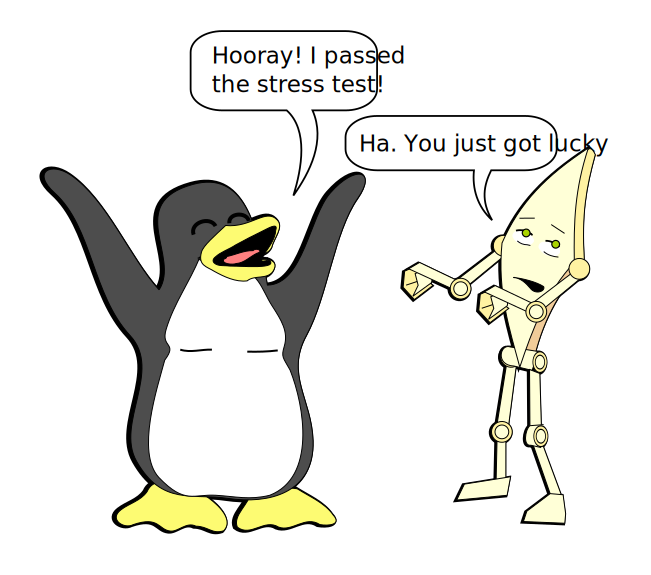
\includegraphics{cartoons/r-2014-Passed-the-stress-test}}
\caption{Passed on Merits?  Or Dumb Luck?}
\ContributedBy{Figure}{fig:cpu:Passed-the-stress-test}{Melissa Broussard}
\end{figure}

이제 질문은, 한편으로는 그 버그가 발생할 확률만을 줄였거나, 관련된 여러개의
버그들 중 하나만을 고쳤거나, 또는 관계없고 효과없는 변경만을 가한게 아니라
정말로 그 버그를 고쳤다는 점을 분명히 하기 위해서 얼마나 많은 테스트를 해야
하는가입니다.
짧게 말해서,
Figure~\ref{fig:cpu:Passed-the-stress-test} 로 암시되는 영원한 질문에 대한 답은
뭘까요?

불행히도, 정직한 답은 절대적인 정확성을 얻기 위해서는 무한한 테스트가
필요하다는 것입니다.
\iffalse

Now the question is just how much testing is required in order to be
certain that
you actually fixed the bug, as opposed to just reducing the probability
of it occurring on the one hand, having fixed only one of several
related bugs on the other hand, or made some ineffectual unrelated
change on yet a third hand.
In short, what is the answer to the eternal question posed by
Figure~\ref{fig:cpu:Passed-the-stress-test}?

Unfortunately, the honest answer is that an infinite amount of testing
is required to attain absolute certainty.
\fi

\QuickQuiz{}
	당신의 쓰레기 봉투에 굉장히 많은 시스템들이 있다고 생각해 봅시다.
	예를 들어, 현재의 클라우드 가격 정책대로라면, 당신은 합리적으로 낮은
	가격에 수많은 CPU 시간을 구입할 수 있습니다.
	모든 실용적인 목적에 있어서의 정확성을 충분히 가져가기 위해서 이 전략을
	사용하지 않나요?
	\iffalse

	Suppose that you had a very large number of systems at your
	disposal.
	For example, at current cloud prices, you can purchase a
	huge amount of CPU time at a reasonably low cost.
	Why not use this approach to get close enough to certainty
	for all practical purposes?
	\fi
\QuickQuizAnswer{
	이 방법은 당신의 검증 무기고에 가치있는 추가물품이 될 수도 있을 겁니다.
	하지만 이 방법은 몇가지 한계점들을 가지고 있습니다:
	\iffalse

	This approach might well be a valuable addition to your
	validation arsenal.
	But it does have a few limitations:
	\fi
	\begin{enumerate}
	\item	일부 버그들은 극단적으로 낮은 발생 가능성을 가지고 있지만, 더도
		아니고 덜도 아니고 고쳐져야 합니다.
		예를 들어, 리눅스 커널의 RCU 구현이 평균적으로 100년의 CPU
		시간에 딱 한번 발생하는 버그를 가지고 있다고 생각해 봅시다.
		100년의 CPU 시간은 가장 싼 클라우드 플랫폼에서라고 해도 상당히
		비싼 가격입니다만, 2011년의 세계에서 1억개의 리눅스 인스턴스
		위에서라면 이 버그는 하루에도 2,000 회 이상의 문제를 일으킬 수
		있을 것으로 예상할 수도 있습니다.
	\item	버그는 당신의 테스트 환경에서는 발생 가능성이 없을 수 있는데,
		이는 당신이 테스트를 하는데에 얼마나 많은 시간을 쏟아붓는가와
		관계없이 당신은 그 버그를 볼 수 없을 것이란 것을 의미합니다.
	\iffalse

	\item	Some bugs have extremely low probabilities of occurrence,
		but nevertheless need to be fixed.
		For example, suppose that the Linux kernel's RCU
		implementation had a bug that is triggered only once
		per century of machine time on average.
		A century of CPU time is hugely expensive even on
		the cheapest cloud platforms, but we could expect
		this bug to result in more than 2,000 failures per day
		on the more than 100 million Linux instances in the
		world as of 2011.
	\item	The bug might well have zero probability of occurrence
		on your test setup, which means that you won't see it
		no matter how much machine time you burn testing it.
	\fi
	\end{enumerate}
	물론, 당신의 코드가 충분히 작다면
	Section~\ref{chp:Formal Verification} 에서와 같이,
	정식적인 검증 절차가 도움이 될 수 있을 겁니다.
	하지만 주의하세요: 당신의 코드의 정식적 검증은 당신의 가정, 요구사항에
	대한 잘못된 이해, 당신이 사용하는 소프트웨어나 하드웨어에 대한 잘못된
	이해, 또는 당신이 증명을 할 생각을 하지 못한 에러에 대해서는 문제를
	찾아내지 못할 겁니다.
	\iffalse

	Of course, if your code is small enough, formal validation
	may be helpful, as discussed in
	Chapter~\ref{chp:Formal Verification}.
	But beware: formal validation of your code will not find
	errors in your assumptions, misunderstanding of the
	requirements, misunderstanding of the software or hardware
	primitives you use, or errors that you did not think to construct
	a proof for.
	\fi
} \QuickQuizEnd

하지만 절대적인 정확성을 포기하고 높은 가능성에 치중하도록 하려 한다고 생각해 봅시다.
그렇다면 우린 이 문제를 해결하는데에 강력한 통계적 도구들을 사용할 수 있습니다.
하지만, 이 섹션은 간단한 통계 도구들에 집중해 봅니다.
이런 도구들은 굉장히 도움이 됩니다만, 이 섹션을 읽는 것이 훌륭한 통계 수업들을
듣는 것을 대체할 수는 없다는 점을 알아두시기 바랍니다.\footnote{
	전 그러기를 강력하게 추천합니다.
	제가 들었던 몇개의 통계 수업들은 제가 그것들을 공부하기 위해 쏟았던
	시간에 비례해서 가치를 제공했습니다.}
\iffalse

But suppose that we are willing to give up absolute certainty in favor
of high probability.
Then we can bring powerful statistical tools to bear on this problem.
However, this section will focus on simple statistical tools.
These tools are extremely helpful, but please note
that reading this section not a substitute
for taking a good set of statistics classes.\footnote{
	Which I most highly recommend.
	The few statistics courses I have taken have provided value
	way out of proportion to the time I spent studying for them.}
\fi

간단한 통계적 도구들을 알아보는걸 시작하기 위해, 우리가 별개적인 테스트를
할것인지 연속적인 테스트를 할것인지 결정해야 합니다.
별개적 테스트는 잘 정의된 개별 테스트 수행들을 갖춥니다.
예를 들어, 리눅스 커널 패치의 부팅 테스트는 별개적 테스트의 한 예입니다.
커널을 부팅해 보고, 그게 부팅되거나 아니거나입니다.
비록 당신은 당신의 커널을 부팅 테스트 하는데에 한시간을 소비할 수도 있긴
하지만, 대부분의 경우에 있어서 커널을 부팅하기 위해 시도한 시도의 횟수와 부팅이
성공한 횟수가 테스트에 소비한 시간의 길이보다 더 흥미로운 것이 될 겁니다.
기능 테스트는 별개적이게 되는 경향이 있습니다.
\iffalse

For our start with simple statistical tools, we need to decide whether
we are doing discrete or continuous testing.
Discrete testing features well-defined individual test runs.
For example, a boot-up test of a Linux kernel patch is an example
of a discrete test.
You boot the kernel, and it either comes up or it does not.
Although you might spend an hour boot-testing your kernel, the number of
times you attempted to boot the kernel and the number of times the
boot-up succeeded would often be of more interest than the length
of time you spent testing.
Functional tests tend to be discrete.
\fi

한편으로는, 만약 제 패치가 RCU 에 관련되어 있다면, 저는 RCU 를 테스트하는 커널
모듈인 rcutorture 를 돌려볼겁니다.
하나의 별개 테스트의 성공적인 마지막에는 로그인 프롬프트 시그널을 띄워주는 커널
부팅과 달리, rcutorture 는 커널이 크래시 나거나 당신이 멈추라고 하기 전까지는
RCU 를 고문하는 것을 지속할 겁니다.
따라서 rcutorture 테스트에 걸리는 시간이 (일반적으로) 당신이 그걸 시작하고 멈춘
시간보다 더 중요하게 됩니다.
따라서, rcutorture 는 많은 스트레스 테스트들을 포함하는 카테고리인 연속적
테스트의 한 예입니다.
\iffalse

On the other hand, if my patch involved RCU, I would probably run
rcutorture, which is a kernel module that, strangely enough, tests RCU.
Unlike booting the kernel, where the appearance of a login prompt
signals the successful end of a discrete test, rcutorture will happily
continue torturing RCU until either the kernel crashes or until you
tell it to stop.
The duration of the rcutorture test is therefore (usually) of more
interest than the number of times you started and stopped it.
Therefore, rcutorture is an example of a continuous test, a category
that includes many stress tests.
\fi

별개 테스트와 연속적 테스트를 운영하는 통계는 몇몇 부분에서 다릅니다.
하지만, 별개 테스트들을 위한 통계는 연속적 테스트를 위한 것보다 더 간단하고
친숙하며, 뿐만아니라 별개 테스트들을 위한 통계는 종종 (약간의 정확성 손실과
함께) 연속적 테스트를 위한 서비스에 사용되기도 합니다.
따라서 우리는 별개 테스트들부터 시작하겠습니다.
\iffalse

The statistics governing discrete and continuous tests differ somewhat.
However, the statistics for discrete tests is simpler and more
familiar than that for continuous tests, and furthermore the
statistics for discrete tests can often be pressed into service
(with some loss of accuracy) for continuous tests.
We therefore start with discrete tests.
\fi

\subsection{Statistics for Discrete Testing}
\label{sec:debugging:Statistics for Discrete Testing}

버그가 한번의 프로그램 수행 사이에 10\,\% 의 발생 확률을 가지고 있고 우리는
프로그램을 다섯번 수행한다고 생각해 봅시다.
최소 한번의 수행은 실패할 확률을 어떻게 계산하면 될까요?
그런 한가지 방법은 다음과 같습니다:
\iffalse

Suppose that the bug had a 10\,\% chance of occurring in
a given run and that we do five runs.
How do we compute that probability of at least one run failing?
One way is as follows:
\fi

\begin{enumerate}
\item	하나의 수행이 성공할 확률을 계산하는데, 이건 90\,\% 입니다.
\item	모든 다섯번의 수행이 성공할 확률을 계산하는데, 이는 0.9 의 5승이어서,
	약 59\,\% 입니다.
\item	두개의 가능성만이 존재합니다: 다섯번의 수행이 모두 성공하거나, 최소
	한번은 실패하거나.
	따라서, 최소 한번은 실패할 확률은 100\,\% 에서 59\,\% 를 제외한
	나머지인 41\,\% 입니다.
\iffalse

\item	Compute the probability of a given run succeeding, which is 90\,\%.
\item	Compute the probability of all five runs succeeding, which
	is 0.9 raised to the fifth power, or about 59\,\%.
\item	There are only two possibilities: either all five runs succeed,
	or at least one fails.
	Therefore, the probability of at least one failure is
	59\,\% taken away from 100\,\%, or 41\,\%.
\fi
\end{enumerate}

하지만, 많은 사람들이 여러 단계보다는 하나의 공식을 사용하는게 더 쉽다고
생각하므로, 설령 당신은 앞의 단계들이 더 편하다고 해도, 한번 해봅시다!
공식을 더 선호하는 사람들을 위해, 한번의 실패할 확률을 $f$ 라고 해봅시다.
그럼 한번의 성공을 할 확률은 $1-f$ 이고, 따라서 $n$ 개의 테스트들이 모두 성공할
확률은:
\iffalse

However, many people find it easier to work with a formula than a series
of steps, although if you prefer the above series of steps, have at it!
For those who like formulas, call the probability of a single failure $f$.
The probability of a single success is then $1-f$ and the probability
that all of $n$ tests will succeed is then:
\fi

\begin{equation}
	S_n = \left(1-f\right)^n
\end{equation}

실패할 확률은 $1-S_n$ , 또는:
\iffalse

The probability of failure is $1-S_n$, or:
\fi

\begin{equation}
	F_n = 1-\left(1-f\right)^n
\label{eq:debugging:Binomial Failure Rate}
\end{equation}

\QuickQuiz{}
	뭐라구요???
	제가 앞의, 각각 10\,\% 실패 확률을 갖는 다섯번의 테스트의 예를 이 공식에
	집어넣어보면 59,050\,\% 를 얻게 되는데 이건 말이 안되잖아요!!!
	\iffalse

	Say what???
	When I plug the earlier example of five tests each with a
	10\,\% failure rate into the formula, I get 59,050\,\% and that
	just doesn't make sense!!!
	\fi
\QuickQuizAnswer{
	당신 말이 맞아요, 전혀 말이 안되죠.

	확률은 0과 1 사이의 숫자여서 당신은 확률을 구하기 위해서는 퍼센티지를
	100 으로 나눠야 함을 기억하세요.
	따라서 10\,\% 의 확률은 0.1 로, 공식에 대입한 확률은 0.4095 값을 얻게
	되는데, 이는 41\,\% 로 반올림 되는데, 이렇게 되면 앞의 결과와 상당히
	일관적이지요.
	\iffalse

	You are right, that makes no sense at all.

	Remember that a probability is a number between zero and one,
	so that you need to divide a percentage by 100 to get a
	probability.
	So 10\,\% is a probability of 0.1, which gets a probability
	of 0.4095, which rounds to 41\,\%, which quite sensibly
	matches the earlier result.
	\fi
} \QuickQuizEnd

따라서 특정 테스트가 10\,\% 의 확률로 실패하고 있다고 해봅시다.
당신의 수정이 정말로 일을 개선시켰다고 99\,\% 확신할 수 있으려면 얼마나 많은
테스트를 수행시켜 봐야 할까요?
\iffalse

So suppose that a given test has been failing 10\,\% of the time.
How many times do you have to run the test to be 99\,\% sure that
your supposed fix has actually improved matters?
\fi

이걸 다르게 질문해 보면 ``실패를 일으킬 확률을 99\,\% 까지 올리려면 얼마나 많은
테스트를 돌려보아야 할까요?'' 입니다.
일단, 최소 하나의 실패를 볼 수 있는 확률이 99\,\% 까지 되도록 테스트를 충분히
많이 돌린다면, 그리고 거기에 실패가 한번도 없다면, 이는 단지 1\,\% 확률의 행운
덕입니다.
그리고 우리가
Equation~\ref{eq:debugging:Binomial Failure Rate} 에 $f=0.1$ 을 집어넣고 $n$ 을
변경시켜보면, 원래의 10\,\% 라는 테스트당 실패 확률에 대해서 43번의 수행이
99.03\,\% 의 최소 한번은 테스트가 실패할 확률을 가져오고, 44번의 수행은
99.03\,\% 의 최소 한번은 실패할 확률을 가져옴을 알 수 있습니다.
따라서 우리가 수정을 한 후에 44번 테스트를 진행하고 실패를 한번도 보지
못한다면, 우리의 수정이 정말로 실제 개선을 만들어냈을 확률이 99\,\% 인
것입니다.
\iffalse

Another way to ask this question is ``How many times would we need
to run the test to cause the probability of failure to rise above 99\,\%?''
After all, if we were to run the test enough times that the probability
of seeing at least one failure becomes 99\,\%, if there are no failures,
there is only 1\,\% probability of this being due to dumb luck.
And if we plug $f=0.1$ into
Equation~\ref{eq:debugging:Binomial Failure Rate} and vary $n$,
we find that 43 runs gives us a 98.92\,\% chance of at least one test failing
given the original 10\,\% per-test failure rate,
while 44 runs gives us a 99.03\,\% chance of at least one test failing.
So if we run the test on our fix 44 times and see no failures, there
is a 99\,\% probability that our fix was actually a real improvement.
\fi

하지만 계속해서 숫자들을
Equation~\ref{eq:debugging:Binomial Failure Rate}
에 집어넣어보는 것은 지켜울 수 있으므로, $n$ 을 풀어봅시다:
\iffalse

But repeatedly plugging numbers into
Equation~\ref{eq:debugging:Binomial Failure Rate}
can get tedious, so let's solve for $n$:
\fi

\begin{eqnarray}
	F_n = 1-\left(1-f\right)^n \\
	1 - F_n = \left(1-f\right)^n \\
	\log \left(1 - F_n\right) = n \; \log \left(1 - f\right)
\end{eqnarray}

마지막으로 요구되는 테스트의 횟수는 다음과 같이 구해집니다:
\iffalse

Finally the number of tests required is given by:
\fi

\begin{equation}
	n = \frac{\log\left(1 - F_n\right)}{\log\left(1 - f\right)}
\label{eq:debugging:Binomial Number of Tests Required}
\end{equation}

Equation~\ref{eq:debugging:Binomial Number of Tests Required} 에
$f=0.1$ 와 $F_n=0.99$ 를 대입해 보면 43.7 이 나오는데, 이는 우리의 수정이 실제
개선을 만들어냈음을 99\,\% 확신하려면 44번의 연속적인 성공적 테스트가 필요함을
의미합니다.
이는 안심스럽게도 앞의 방법에서 얻어진 숫자와 맞아떨어집니다.
\iffalse

Plugging $f=0.1$ and $F_n=0.99$ into
Equation~\ref{eq:debugging:Binomial Number of Tests Required}
gives 43.7, meaning that we need 44 consecutive successful test
runs to be 99\,\% certain that our fix was a real improvement.
This matches the number obtained by the previous method, which
is reassuring.
\fi

\QuickQuiz{}
	Equation~\ref{eq:debugging:Binomial Number of Tests Required} 에서,
	로그의 밑은 10인가요, 2인가요, 또는 $\euler$ 인가요?
	\iffalse

	In Equation~\ref{eq:debugging:Binomial Number of Tests Required},
	are the logarithms base-10, base-2, or base-$\euler$?
	\fi
\QuickQuizAnswer{
	그건 상관 없습니다.
	어떤 밑의 로그를 취하는가에 관계없이 똑같은 답을 얻을 수 있을텐데 그
	결과는 로그 값들 간의 비율이기 때문입니다.
	유일한 제약은 분모와 분자에 둘다 같은 밑을 사용해야 한다는 점입니다.
	\iffalse

	It does not matter.
	You will get the same answer no matter what base of logarithms
	you use because the result is a pure ratio of logarithms.
	The only constraint is that you use the same base for both
	the numerator and the denominator.
	\fi
} \QuickQuizEnd

\begin{figure}[tb]
\centering
\resizebox{2.5in}{!}{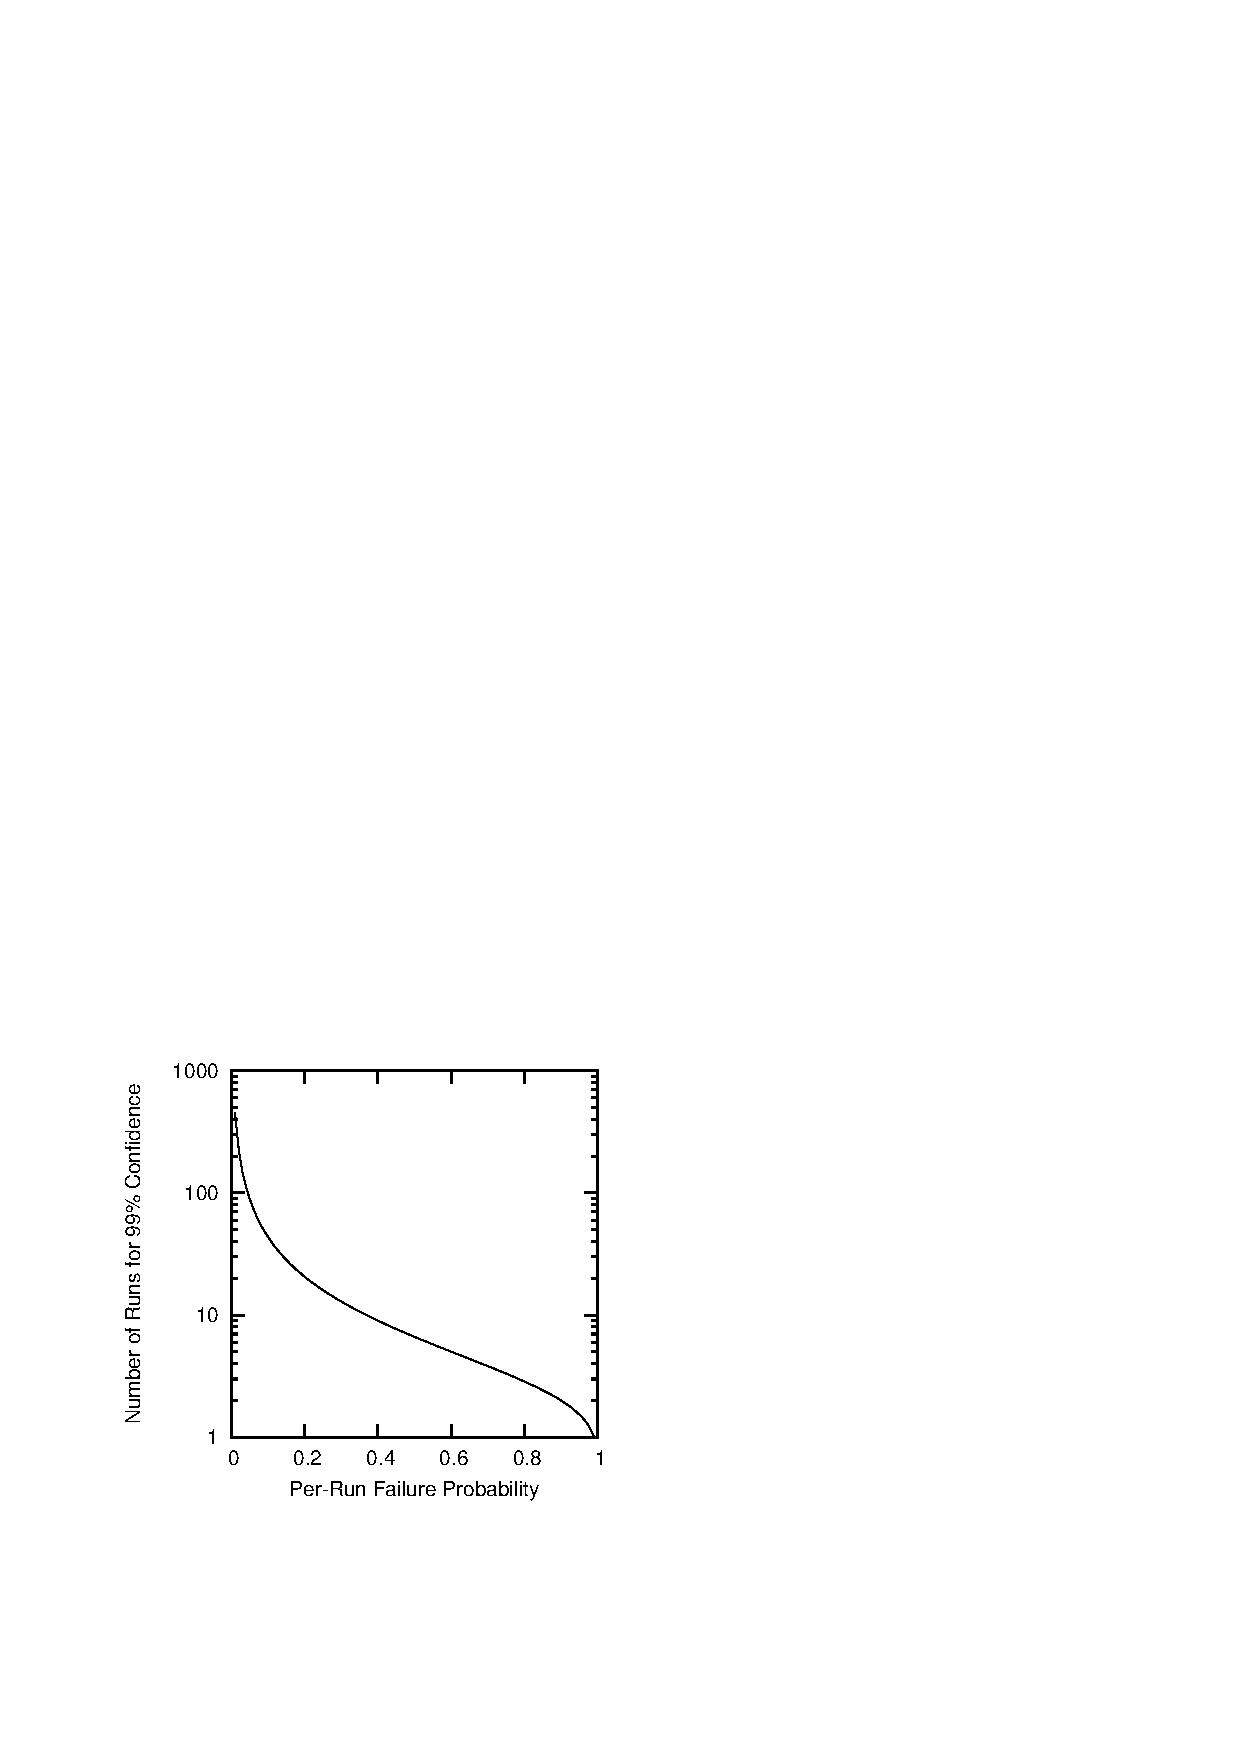
\includegraphics{CodeSamples/debugging/BinomialNRuns}}
\caption{Number of Tests Required for 99 Percent Confidence Given Failure Rate}
\label{fig:debugging:Number of Tests Required for 99 Percent Confidence Given Failure Rate}
\end{figure}

Figure~\ref{fig:debugging:Number of Tests Required for 99 Percent Confidence Given Failure Rate}
는 이 함수를 그래프로 그려보입니다.
놀랍지 않게, 각각의 테스트가 덜 빈번하게 실패할수록, 그 버그가 고쳐졌음을
99\,\% 확신하기 위해선 더 많은 테스트 수행이 필요합니다.
테스트를 실패하게 하는 버그가 오직 1\,\% 의 확률만으로 나타난다면, 애끓는
심정의 458 번의 테스트 수행이 필요합니다.
실패 확률이 줄어들수록, 필요한 테스트 수행 횟수가 증가해서, 실패 확률을 0으로
하려면 무한번의 테스트 수행이 필요해집니다.
\iffalse

Figure~\ref{fig:debugging:Number of Tests Required for 99 Percent Confidence Given Failure Rate}
shows a plot of this function.
Not surprisingly, the less frequently each test run fails, the more
test runs are required to be 99\,\% confident that the bug has been
fixed.
If the bug caused the test to fail only 1\,\% of the time, then a
mind-boggling 458 test runs are required.
As the failure probability decreases, the number of test runs required
increases, going to infinity as the failure probability goes to zero.
\fi

이 이야기의 교훈은 가끔씩만 일어나는 버그를 발견했다면, 실패 확률을 훨씬
높이도록 잘 타겟팅 된 테스트를 사용한다면 테스트 업무가 훨씬 쉬워질 것이란
점입니다.
예를 들어, 타겟이 된 테스트가 실패 확률을 1\,\% 에서 30\,\% 로 늘린다면, 99\,\%
확신을 갖기 위해 필요한 테스트 수행 횟수는 458 회에서 단지 13회까지로 떨어질
겁니다.
\iffalse

The moral of this story is that when you have found a rarely occurring
bug, your testing job will be much easier if you can come up with
a carefully targeted test with a much higher failure rate.
For example, if your targeted test raised the failure rate from 1\,\%
to 30\,\%, then the number of runs required for 99\,\% confidence
would drop from 458 test runs to a mere thirteen test runs.
\fi

하지만 이 열세번의 테스트 수행은 당신의 수정 사항이 ``어떤 개선'' 을
만들어냈다는 데에 99\,\% 의 확신만을 제공합니다.
당신이 원하는건 그게 아니라 당신의 수정 사항이 실패 확률을 10배 가량 줄인
것이라는 99\,\%의 확신이라고 생각해 봅시다.
얼마나 많은 실패하지 않는 테스트 수행이 필요할까요?
\iffalse

But these thirteen test runs would only give you 99\,\% confidence that
your fix had produced ``some improvement''.
Suppose you instead want to have 99\,\% confidence that your fix reduced
the failure rate by an order of magnitude.
How many failure-free test runs are required?
\fi

30\,\% 실패 확률에서 10배 개선된다면 3\,\% 의 실패 확률입니다.
이 숫자들을
Equation~\ref{eq:debugging:Binomial Number of Tests Required} 에 집어넣으면
다음과 같은 결과가 나옵니다:
\iffalse

An order of magnitude improvement from a 30\,\% failure rate would be
a 3\,\% failure rate.
Plugging these numbers into
Equation~\ref{eq:debugging:Binomial Number of Tests Required} yields:
\fi

\begin{equation}
	n = \frac{\log\left(1 - 0.99\right)}{\log\left(1 - 0.03\right)} = 151.2
\end{equation}

따라서 우리의 10배 개선을 위해서는 대략 10배 이상의 테스트가 필요합니다.
확신은 불가능하고, 높은 확률은 상당히 비쌉니다.
테스트들이 수행은 더 빠르게 되고 실패는 더 잘 일어나도록 분명하게 만드는 것이
높은 수준의 안정성을 갖는 소프트웨어를 개발하는데에 있어 핵심의 기술들입니다.
이런 기술들은
Section~\ref{sec:debugging:Hunting Heisenbugs} 에서 다루겠습니다.
\iffalse

So our order of magnitude improvement requires roughly an order of
magnitude more testing.
Certainty is impossible, and high probabilities are quite expensive.
Clearly making tests run more quickly and making failures more probable
are essential skills in the development of highly reliable software.
These skills will be covered in
Section~\ref{sec:debugging:Hunting Heisenbugs}.
\fi

\subsection{Abusing Statistics for Discrete Testing}
\label{sec:debugging:Abusing Statistics for Discrete Testing}

하지만 당신이 열번 수행하면 세번은 실패하는 연속적인 테스트를 가지고 있고, 그
실패를 유발했다고 당신이 생각하는 버그를 고쳤다고 생각해 봅시다.
당신이 실패의 가능성을 줄였다는 점을 99\,\% 확신하려면 얼마나 많은 횟수의 실패
없는 테스트를 수행해야 할까요?
\iffalse

But suppose that you have a continuous test that fails about three
times every ten hours, and that you fix the bug that you believe was
causing the failure.
How long do you have to run this test without failure to be 99\,\% certain
that you reduced the probability of failure?
\fi

통계를 극단적으로 해치지 않으면서, 우리는 간단히 한시간동안의 수행을 30\,\% 의
실패 가능성을 가진 별개의 테스트로 재정의 할 수 있을겁니다.
그렇다면 앞의 섹션에서의 결과는 테스트가 13시간동안 실패 없이 돌아간다면,
우리의 수정사항은 실제로 프로그램의 안정성을 개선했을 가능성이 99\,\% 라고 이야기
하게 됩니다.
\iffalse

Without doing excessive violence to statistics, we could simply
redefine a one-hour run to be a discrete test that has a 30\,\%
probability of failure.
Then the results of in the previous section tell us that if the test
runs for 13 hours without failure, there is a 99\,\% probability that
our fix actually improved the program's reliability.
\fi

교리적인 통계학자는 이런 접근을 허락하지 않을겁니다만, 슬픈 사실은 이런 종류의
통계 방법론의 오용으로 인해 발생하는 에러들은 당신의 프로그램의 실패 확률의
측정에서 피할 수 없는 에러들보다는 훨씬 작다는 것입니다.
더도 아니고 덜도 아니고, 다음 섹션에서는 약간 덜 사기적인 방법을 설명합니다.
\iffalse

A dogmatic statistician might not approve of this approach, but the
sad fact is that the errors introduced by this sort of abuse of
statistical methodology are usually quite small compared to the
errors inherent in your measurements of your program's failure rates.
Nevertheless, the next section describes a slightly less dodgy approach.
\fi

\subsection{Statistics for Continuous Testing}
\label{sec:debuggingStatistics for Continuous Testing}

실패 확률을 위한 기본적인 공식은 Poisson 분포입니다:
\iffalse

The fundamental formula for failure probabilities is the Poisson
distribution:
\fi

\begin{equation}
	F_m = \frac{\lambda^m}{m!} \euler^{-\lambda}
\label{eq:debugging:Poisson Probability}
\end{equation}

여기서 $F_m$ 은 테스트에서 $m$ 실패의 확률이고 $\lambda$ 는 단위시간 동안
예상되는 실패 비율입니다.
더 엄격한 유도는 더 나은 확률에 대한 교제들에서 찾아볼 수 있을텐데, 예를 들어
Feller 의 고전인 ``An Introduction to Probability Theory and Its
Application''~\cite{Feller58} 가 있으며, 더 직관적인 접근법은 이 책의 첫번째
수정본~\cite{McKenney2014ParallelProgramming-e1} 에서 찾아볼 수 있을 겁니다.
\iffalse

Here $F_m$ is the probability of $m$ failures in the test and
$\lambda$ is the expected failure rate per unit time.
A rigorous derivation may be found in any advanced probability
textbook, for example, Feller's classic ``An Introduction to Probability
Theory and Its Applications''~\cite{Feller58}, while a more
intuitive approach may be found in the first edition of
this book~\cite{McKenney2014ParallelProgramming-e1}.
\fi

Section~\ref{sec:debugging:Abusing Statistics for Discrete Testing} 에서의
예제를 Poisson 분포를 이용해서 다시 한번 작업해 봅시다.
이 예제가 시간당 30\,\% 실패 확률을 갖는 테스트에 관련된 거라는 점, 그리고
질문은 의심되는 수정사항에 대해 그 수정사항이 정말로 실패 확률을 줄였다고
99\,\% 확신하기 위해서는 테스트가 얼마나 오래 실패 없이 돌아갈 수 있어야 하는가
라는 점을 다시 상기합시다.
이 경우에, $\lambda$ 는 0이므로,
Equation~\ref{eq:debugging:Poisson Probability} 는 다음과 같이 간략화 됩니다:
\iffalse

Let's try reworking the example from
Section~\ref{sec:debugging:Abusing Statistics for Discrete Testing}
using the Poisson distribution.
Recall that this example involved a test with a 30\,\% failure rate per
hour, and that the question was how long the test would need to run
error-free
on a alleged fix to be 99\,\% certain that the fix actually reduced the
failure rate.
In this case, $m$ is zero, so that
Equation~\ref{eq:debugging:Poisson Probability} reduces to:
\fi

\begin{equation}
	F_0 =  \euler^{-\lambda}
\end{equation}

이걸 풀기 위해서는 $F_0$ 를 0.01 로 설정해야 하며, 여기서 $\lambda$ 를 구해
보면:
\iffalse

Solving this requires setting $F_0$
to 0.01 and solving for $\lambda$, resulting in:
\fi

\begin{equation}
	\lambda = - \ln 0.01 = 4.6
\end{equation}

우리가 시간당 $0.3$ 실패를 가지므로, 요구되는 시간은 $4.6/0.3 = 14.3$ 으로,
Section~\ref{sec:debugging:Abusing Statistics for Discrete Testing} 에서 사용한
방법으로 계산한 13시간과 10\,\% 오차 내에 있습니다.
일반적으로는 실패 확률이 10\,\% 내라는 것은 알지 못할 것이라는 점을 놓고 보면,
이는
Section~\ref{sec:debugging:Abusing Statistics for Discrete Testing} 에서의
방법이 상당히 많은 상황에서 Poisson 분포를 대체할 수 있는 훌륭하고 충분한
대체제임을 말합니다.

더 일반적으로 말해서, 단위시간당 $n$ 실패를 갖는다면, 그리고 어떤 수정사항이
실패 확률을 줄였다고 $P$\,\% 확신하려면 다음의 공식을 사용할 수 있습니다:
\iffalse

Because we get $0.3$ failures per hour, the number of hours required
is $4.6/0.3 = 14.3$, which is within 10\,\% of the 13 hours
calculated using the method in
Section~\ref{sec:debugging:Abusing Statistics for Discrete Testing}.
Given that you normally won't know your failure rate to within 10\,\%,
this indicates that the method in
Section~\ref{sec:debugging:Abusing Statistics for Discrete Testing}
is a good and sufficient substitute for the Poisson distribution in
a great many situations.

More generally, if we have $n$ failures per unit time, and we want to
be $P$\,\% certain that a fix reduced the failure rate, we can use the
following formula:
\fi

\begin{equation}
	T = - \frac{1}{n} \ln \frac{100 - P}{100}
\label{eq:debugging:Error-Free Test Duration}
\end{equation}

\QuickQuiz{}
	어떤 버그가 평균적으로 시간당 세번의 테스트 실패를 유발한다고 생각해
	봅시다.
	수정사항이 실패의 확률을 상당히 줄였음을 99.9\,\% 증명할 수 있는 증거를
	위해서는 테스트는 에러 없이 얼마나 오래 돌아가야만 할까요?
	\iffalse

	Suppose that a bug causes a test failure three times per hour
	on average.
	How long must the test run error-free to provide 99.9\,\%
	confidence that the fix significantly reduced the probability
	of failure?
	\fi
\QuickQuizAnswer{
	Equation~\ref{eq:debugging:Error-Free Test Duration} 에서 $n$ 은 $3$
	으로, 그리고 $P$ 를 $99.9$ 로 놓으면, 결과는 다음과 같습니다:
	\iffalse

	We set $n$ to $3$ and $P$ to $99.9$ in
	Equation~\ref{eq:debugging:Error-Free Test Duration}, resulting in:
	\fi

	\begin{equation}
		T = - \frac{1}{3} \ln \frac{100 - 99.9}{100} = 2.3
	\end{equation}

	테스트가 실패하지 않은채 2.3 시간동안 돌아간다면, 우린 해당 수정사항이
	실패 가능성을 줄였음을 99.9\,\% 확신할 수 있습니다.
	\iffalse

	If the test runs without failure for 2.3 hours, we can be 99.9\,\%
	certain that the fix reduced the probability of failure.
	\fi
} \QuickQuizEnd

앞에서와 같이, 버그가 덜 빈번하게 발생하고 필요한 확신의 수준이 클수록 에러
없이 테스트가 수행되어야 하는 시간이 길어집니다.

테스트가 매 시간마다 한번씩 실패하지만, 버그 수정 후, 24시간의 테스트에서
두번만 테스트가 수행중 실패했다고 생각해 봅시다.
해당 버그로 이끌어진 실패는 무작위적으로 발생한다고 하면, 두번째 테스트
수행에서의 적은 수의 실패들은 무작위적 기회로 발생한 것일 확률은 얼마일까요?
달리 말해서, 해당 수정이 정말로 버그에 대해서 어떤 영향을 끼쳤다고 얼마나
확신해야 하는걸까요?
이 확률은 다음과 같이
Equation~\ref{eq:debugging:Poisson Probability} 를 합하는 것으로 구할 수 있을
겁니다:
\iffalse

As before, the less frequently the bug occurs and the greater the
required level of confidence, the longer the required error-free test run.

Suppose that a given test fails about once every hour, but after a bug
fix, a 24-hour test run fails only twice.
Assuming that the failure leading to the bug is a random occurrence,
what is the probability that the small number of
failures in the second run was due to random chance?
In other words, how confident should we be that the fix actually
had some effect on the bug?
This probability may be calculated by summing
Equation~\ref{eq:debugging:Poisson Probability} as follows:
\fi

\begin{equation}
	F_0 + F_1 + \dots + F_{m - 1} + F_m =
		\sum_{i=0}^m \frac{\lambda^i}{i!} \euler^{-\lambda}
\end{equation}

이는 Poisson 누적분포지수 (cumulative distribution function) 인데, 더
간단하게는 다음과 같이 쓰일 수 있습니다:
\iffalse

This is the Poisson cumulative distribution function, which can be
written more compactly as:
\fi

\begin{equation}
	F_{i \le m} = \sum_{i=0}^m \frac{\lambda^i}{i!} \euler^{-\lambda}
\label{eq:debugging:Possion CDF}
\end{equation}

여기서 $m$ 은 긴 시간동안의 테스트에서의 에러의 갯수 (이 경우, 2) 이고,
$\lambda$ 는 긴 시간동안의 테스트에서 발생하리라 예측된 에러들의 갯수입니다 (이
경우, 24).
$m=2$ 와 $\lambda=24$ 를 이 수식에 대입하면 약 $1.2 \times 10^{-8}$ 으로 2
언저리의 확률이 나오는데, 달리 말해서, 해당 수정 사항이 정말로 해당 버그에 어떤
관계를 맺었음을 말하는 높은 수준의 증거를 가질 수 있는 겁니다.\footnote{
	물론, 이 결과가 남은 두개의 실패들을 만들어낸 버그(들)을 찾아내고
	고쳐야 한다는 사실에 대해 변명거리가 되지 않습니다!}
\iffalse

Here $m$ is the number of errors in the long test run
(in this case, two) and $\lambda$ is expected number of errors
in the long test run (in this case, 24).
Plugging $m=2$ and $\lambda=24$ into this expression gives the probability
of two or fewer failures as about
$1.2 \times 10^{-8}$, in other words, we have a high level of confidence
that the fix actually had some relationship to the bug.\footnote{
	Of course, this result in no way excuses you from finding and
	fixing the bug(s) resulting in the remaining two failures!}
\fi

\QuickQuiz{}
	이 모든 계승식 (factorial) 들과 지수식 (exponential) 들을 더하고 있는건
	진짜 고통스럽습니다.
	좀 더 편한 길은 없나요?
	\iffalse

	Doing the summation of all the factorials and exponentials
	is a real pain.
	Isn't there an easier way?
	\fi
\QuickQuizAnswer{
	한가지 방법은 ``maxiam'' 라는 이름의 오픈 소스 기호 논리학 조작
	프로그램을 사용하는 것입니다.
	많은 Debian 기반 리눅스 배포본의 일부분인 이 프로그램을 일단 설치하면,
	이걸 수행하고 \co{load(distrib);} 커맨드를 넣고 이어서
	\co{bfloat(cdf_poisson(m,l));} 커맨드들의 숫자들을 아무거나 넣을 수
	있는데, 여기서 \co{m} 은 $m$ 을 위한 원하는 값을 봐꾸고 \co{l} 은
	원하는 $\lambda$ 값으로 바꿔야 할 겁니다.
	\iffalse

	One approach is to use the open-source symbolic manipulation
	program named ``maxima''.
	Once you have installed this program, which is a part of many
	Debian-based Linux distributions, you can run it and give the
	\co{load(distrib);} command followed by any number of
	\co{bfloat(cdf_poisson(m,l));} commands, where the \co{m}
	is replaced by the desired value of $m$ and the \co{l}
	is replaced by the desired value of $\lambda$.
	\fi

	구체적으로는, \co{bfloat(cdf_poisson(2,24));} 커맨드는
	\co{1.181617112359357b-8} 을 내놓는데, 이는
	Equation~\ref{eq:debugging:Possion CDF} 로 구해진 값과 맞아
	떨어집니다.

	대안적으로는,
	Section~\ref{sec:debugging:Abusing Statistics for Discrete Testing}
	에서 설명하는 rough-and-ready 방법을 사용할 수 있습니다.
	\iffalse

	In particular, the \co{bfloat(cdf_poisson(2,24));} command
	results in \co{1.181617112359357b-8}, which matches the value
	given by Equation~\ref{eq:debugging:Possion CDF}.

	Alternatively, you can use the rough-and-ready method described in
	Section~\ref{sec:debugging:Abusing Statistics for Discrete Testing}.
	\fi
} \QuickQuizEnd

\QuickQuiz{}
	하지만 잠시만요!!!
	실패들의 \emph{어떤} 횟수가 있어야 한다는 (실패가 없을 수 있다는
	가능성을 포함해서) 점을 놓고 보면,
	Equation~\ref{eq:debugging:Possion CDF} 에 보여진 더하기는 $m$ 을 $1$
	로 놓으면 무한대가 되지 않나요?
	\iffalse

	But wait!!!
	Given that there has to be \emph{some} number of failures
	(including the possibility of zero failures),
	shouldn't the summation shown in
	Equation~\ref{eq:debugging:Possion CDF}
	approach the value $1$ as $m$ goes to infinity?
	\fi
\QuickQuizAnswer{
	실제로 그래야 합니다.
	그리고 그렇지요.

	이를 알아보기 위해, $\euler^{-\lambda}$ 는 $i$ 에 의존되지 않는데, 이는
	다음과 같이 더하기에서 빠져나올 수 있음을 의미함을 보세요:
	\iffalse

	Indeed it should.
	And it does.

	To see this, note that $\euler^{-\lambda}$ does not depend on $i$,
	which means that it can be pulled out of the summation as follows:
	\fi

	\begin{equation}
		\euler^{-\lambda} \sum_{i=0}^\infty \frac{\lambda^i}{i!}
	\end{equation}

	남은 더하기는 정확히 $\euler^\lambda$ 를 위한 Taylor 시리즈로, 다음과
	같이 됩니다:
	\iffalse

	The remaining summation is exactly the Taylor series for
	$\euler^\lambda$, yielding:
	\fi

	\begin{equation}
		\euler^{-\lambda} \euler^\lambda
	\end{equation}

	이 두개의 지수식들은 서로 상반되므로 무시되어서 정확히 요구된 대로 $1$
	이 됩니다.
	\iffalse

	The two exponentials are reciprocals, and therefore cancel,
	resulting in exactly $1$, as required.
	\fi
} \QuickQuizEnd

이 Poisson 분포는 테스트 결과를 분석하기 위한 강력한 도구입니다만 이 마지막
예에서는 24시간동안의 테스트 수행에서의 두개의 실패들이 남아있다는게
사실입니다.
그런 낮은 실패 확률은 매우 긴 테스트 수행을 필요로 하게 됩니다.
다음 섹션에서는 이 상황을 개선하기 위한 반직관적인 방법들을 논해봅니다.
\iffalse

The Poisson distribution is a powerful tool for analyzing test results,
but the fact is that in this last example there were still two remaining
test failures in a 24-hour test run.
Such a low failure rate results in very long test runs.
The next section discusses counter-intuitive ways of improving this situation.
\fi

\subsection{Hunting Heisenbugs}
\label{sec:debugging:Hunting Heisenbugs}

이런 생각을 해보는게 heisenbug 의 설명에 도움이 됩니다:
추적 기능과 단정문을 추가하는 것은 버그의 발생 가능성을 줄여버릴 수 있습니다.
그리고 이게 바로 극단적으로 가벼운 추적기능과 단정문 메커니즘이 그렇게 중요한
이유입니다.
\iffalse

This line of thought also helps explain heisenbugs:
adding tracing and assertions can easily reduce the probability
of a bug appearing, which
is why extremely lightweight tracing and assertion mechanism are
so critically important.
\fi

``heisenbug'' 란 용어는 특정 입자의 위치와 속도를 어떤 특정 시점에 정량화 하는
것은 불가능하다는, 양자 물리학의 하이젠버그 불확정성
원리~\cite{WeinerHeisenberg1927Uncertain} (Heisenberg Uncertainty Principle)
에서 나왔습니다.
해당 입자의 위치를 좀 더 정확하게 측정하려는 모든 시도는 그것의 속도에 대한
불확정성을 더욱 증가시키는 결과를 낳습니다.
살짝 비슷한 효과가 heisenbug 에 대해서도 발생합니다: heisenbug 를 추적하려는
시도들은 그 버그의 증상을 철저히 바꿔버리거나 완전히 사라져 버리기조차 하게
합니다.\footnote{
	``Heisenbug'' 라는 용어는 잘못된 호칭인데, 대부분의 heisenbug 들은 고전
	물리학의 \emph{관측자 효과} 로 완전히 설명되기 때문입니다.
	그러나, ``heisenbug'' 라는 이름이 이미 사용되어버렸습니다.}

\iffalse

The term ``heisenbug'' was inspired by the Heisenberg Uncertainty
Principle from quantum physics, which states that it is impossible to
exactly quantify a given particle's position and velocity at any given
point in time~\cite{WeinerHeisenberg1927Uncertain}.
Any attempt to more accurately measure that particle's position will
result in increased uncertainty of its velocity.
A roughly similar effect occurs for heisenbugs: attempts to track down
the heisenbug causes it to radically change its symptoms or even disappear
completely.\footnote{
	The term ``heisenbug'' is a misnomer, as most heisenbugs are
	fully explained by the \emph{observer effect} from classical
	physics.
	Nevertheless, the name ``heisenbug'' has stuck.}
\fi

물리학 방면에서 이 문제의 이름에 대한 영감을 받았다면, 그에 대한 해결책을
위해서도 물리학 방면을 찾아보는것이 논리적입니다.
다행히도, 입자 물리학은 그에 대한 일을 하고 있습니다:
Heisenbug 를 섬멸하기 위해 anti-heisenbug 를 창조하면 어떨까요?
또는, 좀 더 정확히 말하자면, heisenbug 의 heisen 스러움을 없애기 위해서?

이 섹션은 그러기 위한 몇가지 방법들을 설명합니다:
\iffalse

If the field of physics inspired the name of this problem, it is only
logical that the field of physics should inspire the solution.
Fortunately, particle physics is up to the task:
Why not create an anti-heisenbug to annihilate the heisenbug?
Or, perhaps more accurately, to annihilate the heisen-ness of
the heisenbug?

This section describes a number of ways to do just that:
\fi

\begin{enumerate}
\item	경주조건을 일으키기 쉬운 영역들에 딜레이를 추가하기.
\item	워크로드의 강도를 증가시키기.
\item	의심스러운 서브시스템들을 격리시켜서 테스트하기.
\item	일반적이지 않은 이벤트들을 시뮬레이션 해보기.
\item	실수에 가까운 것들의 수를 세어보기.
\iffalse

\item	Add delay to race-prone regions.
\item	Increase workload intensity.
\item	Test suspicious subsystems in isolation.
\item	Simulate unusual events.
\item	Count near misses.
\fi
\end{enumerate}

특정 heisenbug 를 위한 anti-heisenbug 를 만들어내는건 과학이라기보다는 예술에
가깝습니다만, 다음 섹션들은 anti-heisenbug 의 관련된 것들을 만들어내는데 몇가지
팁을 줄겁니다.
이것들은 토론 섹션,
Section~\ref{sec:debugging:Heisenbug Discussion}
에서 이어집니다.
\iffalse

Although producing an anti-heisenbug for a given heisenbug is more an
art than a science, the following sections give some tips on
generating the corresponding species of anti-heisenbug.
These are followed by a discussion section,
Section~\ref{sec:debugging:Heisenbug Discussion}.
\fi

\subsubsection{Add Delay}
\label{sec:debugging:Add Delay}

Section~\ref{sec:count:Why Isn't Concurrent Counting Trivial?} 의 카운트가
누실되는 코드를 생각해 봅시다.
여기에 \co{printf()} 문을 집어넣는 행위는 누실되는 카운트 엄청나게 줄이거나
심지어 없애버릴 수도 있을 겁니다.
하지만, 읽어오고-더하고-저장하는 시퀀스를 읽어오고-더하고-기다리고-저장하는
시퀀스로 바꾸는 것은 누실되는 카운트의 발생률을 엄청나게 증가시킬 겁니다
(해보세요!).
경주 상황에 관련되어 있는 버그를 일단 발견했다면, 이런 식으로 딜레이를 추가하는
것으로 anti-heisenbug 를 만들어내는게 많은 경우에 가능합니다.
\iffalse

Consider the count-lossy code in
Section~\ref{sec:count:Why Isn't Concurrent Counting Trivial?}.
Adding \co{printf()} statements will likely greatly reduce or even
eliminate the lost counts.
However, converting the load-add-store sequence to a load-add-delay-store
sequence will greatly increase the incidence of lost counts (try it!).
Once you spot a bug involving a race condition, it is frequently possible
to create an anti-heisenbug by adding delay in this manner.
\fi

물론, 이는 첫째로 경주 상황을 어떻게 찾아야 하는지에 대한 질문을 이끌어 냅니다.
이건 약간 어둠의 예술입니다만, 그것들을 찾기 위해 할 수 있는 것들이 몇가지
있습니다.
\iffalse

Of course, this begs the question of how to find the race condition in
the first place.
This is a bit of a dark art, but there are a number of things you can
do to find them.
\fi

한가지 방법은, 경주 조건은 많은 경우에 그 경주에 관련된 데이터를 오염시키는
결과를 이끌어 냄을 인식하는 것입니다.
따라서 모든 오염된 데이터의 동기화를 두번씩 체크하는 것은 좋은 습관입니다.
설령 당장은 그 경주 조건을 인식할 수 없다고 해도, 오염된 데이터로의 액세스 전과
후에 딜레이를 추가하는 것은 실패 확률을 바꿀 것입니다.
딜레이들을 잘 조직된 형태 (ex: 이진 탐색) 로 넣고 빼는 것으로, 경주 조건의
동작에 대해 좀 더 알 수 있을 겁니다.
\iffalse

One approach is to recognize that race conditions often end up corrupting
some of the data involved in the race.
It is therefore good practice to double-check the synchronization of
any corrupted data.
Even if you cannot immediately recognize the race condition, adding
delay before and after accesses to the corrupted data might change
the failure rate.
By adding and removing the delays in an organized fashion (e.g., binary
search), you might learn more about the workings of the race condition.
\fi

\QuickQuiz{}
	만약 그 오염이 어떤 관계없는 포인터에 영향을 끼쳐서 그 포인터를
	따라가서 오염을 일으키는 경우에 이 방법은 어떻게 도움을 줄 수
	있을까요???
	\iffalse

	How is this approach supposed to help if the corruption affected some
	unrelated pointer, which then caused the corruption???
	\fi
\QuickQuizAnswer{
	실제로, 그런 상황이 일어날 수 있습니다.
	많은 CPU 들이 그런 관계없는 포인터를 찾아내는 것을 도울 수 있는
	하드웨어 디버깅 기능을 가지고 있습니다.
	뿐만 아니라, core dump 를 가지고 있다면, 메모리의 오염된 영역을
	가리키는 포인터들을 위해 core dump 를 조사할 수 있습니다.
	또한 오염의 데이터 구조를 살펴보고, 그 구조와 맞아떨어지는 포인터들을
	체크해 볼수도 있습니다.
	\iffalse

	Indeed, that can happen.
	Many CPUs have hardware-debugging facilities that can help you
	locate that unrelated pointer.
	Furthermore, if you have a core dump, you can search the core
	dump for pointers referencing the corrupted region of memory.
	You can also look at the data layout of the corruption, and
	check pointers whose type matches that layout.
	\fi

	또한 한발자국 떨어져서 프로그램을 구성하는 모듈들을 더 혹독하게 테스트
	해볼 수 있는데, 이는 오염을 그에 책임이 있는 모듈로 국한시킬 겁니다.
	만약 이게 오염을 사라지게 한다면, 각각의 모듈에서 노출된 함수들의 인자
	체크를 더 추가해 보는 걸 고려해 보세요.

	더도 아니고 덜도 아니고, 이건 어려운 문제인데, 그게 제가 ``약간 어둠의
	예술'' 이라는 말을 사용한 이유입니다.
	\iffalse

	You can also step back and test the modules making up your
	program more intensively, which will likely confine the corruption
	to the module responsible for it.
	If this makes the corruption vanish, consider adding additional
	argument checking to the functions exported from each module.

	Nevertheless, this is a hard problem, which is why I used the
	words ``a bit of a dark art''.
	\fi
} \QuickQuizEnd

또다른 중요한 방법은 소프트웨어와 하드웨어 구성을 다양하게 해가면서 실패 확률의
통계적으로 심각한 차이를 찾아보는 것입니다.
그러고 나면 실패 확률에 가장 커다란 차이를 만들어낸 소프트웨어나 하드웨어 구성
변경점에 의해 암시되는 코드를 더 집중적으로 보는 것입니다.
예를 들어, 그 코드를 격리시켜서 테스트 해보는 것도 도움이 될 수 있을 겁니다.
\iffalse

Another important approach is to
vary the software and hardware configuration and look for statistically
significant differences in failure rate.
You can then look more intensively at the code implicated by the
software or hardware configuration changes that make the greatest
difference in failure rate.
It might be helpful to test that code in isolation, for example.
\fi

소프트웨어 구성의 한가지 중요한 측면은 변경의 역사인데, 이게 바로
\co{git bisect} 이 유용한 이유입니다.
변경 역사의 이등분된 한쪽은 heisenbug 의 원리에 의해 매우 가치있는 단서를
제공할 수 있습니다.
\iffalse

One important aspect of software configuration is the history of
changes, which is why \co{git bisect} is so useful.
Bisection of the change history can provide very valuable clues as
to the nature of the heisenbug.
\fi

\QuickQuiz{}
	하지만 제가 그렇게 이등분을 통한 탐색을 해봤는데, 결국 나온 범인은
	거대한 커밋이었어요.
	이제 뭘 해야 하죠?
	\iffalse

	But I did the bisection, and ended up with a huge commit.
	What do I do now?
	\fi
\QuickQuizAnswer{
	커다란 커밋이요?
	그건 참 부끄러운 일입니다!
	이건 왜 당신이 커밋들을 작게 유지할 것이라 기대되는지에 대한 한가지
	이유일 뿐입니다.

	그리고 그게 당신의 답입니다: 해당 커밋을 바이트 단위의 조각들로 쪼개고
	그 조각들을 다시 이진탐색 하세요.
	제 경험상으로, 그 커밋을 쪼개는 일 자체는 대부분의 경우에 그 버그를
	상당히 분명하게 만들기에 충분합니다.
	\iffalse

	A huge commit?
	Shame on you!
	This is but one reason why you are supposed to keep the commits small.

	And that is your answer: Break up the commit into bite-sized
	pieces and bisect the pieces.
	In my experience, the act of breaking up the commit is often
	sufficient to make the bug painfully obvious.
	\fi
} \QuickQuizEnd

어떻게든 의심스러운 코드 영역을 찾아냈다면, 이제 당신은 실패의 확률을
증가시키기 위해서 딜레이들을 넣을 수 있습니다.
앞서서 우리가 본 것처럼, 실패의 확률을 증가시키는 것은 관련된 수정사항에 대한
높은 신뢰를 얻기 쉽게 해줍니다.

하지만, 일반적인 디버깅 테크닉들을 사용해서 그런 문제를 추적하는 것은 어떤
경우에는 상당히 복잡합니다.
뒤따르는 섹션들은 몇가지 다른 대안들을 제시합니다.
\iffalse

However you locate the suspicious section of code, you can then introduce
delays to attempt to increase the probability of failure.
As we have seen, increasing the probability of failure makes it much
easier to gain high confidence in the corresponding fix.

However, it is sometimes quite difficult to track down the problem using
normal debugging techniques.
The following sections present some other alternatives.
\fi

\subsubsection{Increase Workload Intensity}
\label{sec:debugging:Increase Workload Intensity}

특정 테스트 셋이 특정 서브시스템에는 상대적으로 적은 스트레스를 가해서 타이밍에
대한 작은 변화가 heisenbug 를 사라지게 할 수 있게 되는 경우는 흔합니다.
이런 경우를 위한 anti-heisenbug 를 만들어내는 한가지 방법은 워크로드의 강도를
증가시키는 것으로, 이는 버그가 나타날 확률을 올리는 기회를 갖습니다.
만약 확률이 충분히 증가한다면, 버그가 사라지게 하지 않으면서도 추적 기능과 같은
가벼운 디버깅 기능들을 추가할 수도 있을 겁니다.

워크로드의 강도를 어떻게 증가시킬 수 있을까요?
이는 프로그램에 따라 다르긴 합니다만, 여기 몇가지 시도해볼만한 것들이 있습니다:
\iffalse

It is often the case that a given test suite places relatively
low stress on a given subsystem, so that a small change in timing
can cause a heisenbug to disappear.
One way to create an anti-heisenbug for this case is to increase
the workload intensity, which has a good chance of increasing the
probability of the bug appearing.
If the probability is increased sufficiently, it may be possible to
add lightweight diagnostics such as tracing without causing the
bug to vanish.

How can you increase the workload intensity?
This depends on the program, but here are some things to try:
\fi

\begin{enumerate}
\item	CPU 들을 추가합니다.
\item	프로그램이 네트워킹을 사용한다면, 더 많은 네트워크 어댑터들과 원격의
	시스템들을 더 많이 추가하거나 더 빠른 것으로 바꾸세요.
\item	프로그램이 문제가 발생할 때 무거운 I/O 를 하고 있다면, (1) 더 많은
	저장장치를 추가하거나, (2) 디스크를 SSD 로 대체하거나 하는 식으로 더
	빠른 저장 장치를 사용하거나, (3) 대용량 저장장치를 메인 메모리로
	대체하기 위해 RAM 기반 파일시스템을 사용하세요.
\item	예를 들어 병렬 행렬 곱셈을 하고 있다면 행렬의 크기를 바꾸는 식으로
	문제의 크기를 바꾸세요.
	더 큰 문제들은 더 많은 복잡도를 가져올 수 있습니다만, 더 작은 문제들은
	종종 경쟁의 수준을 증가시킵니다.
	더 크게 해야 할지 작게 해야 할지 모르겠다면, 그냥 둘 다 해보세요.
\iffalse

\item	Add more CPUs.
\item	If the program uses networking, add more network adapters
	and more or faster remote systems.
\item	If the program is doing heavy I/O when the problem occurs,
	either (1) add more storage devices, (2) use faster storage
	devices, for example, substitute SSDs for disks,
	or (3) use a RAM-based filesystem to substitute main
	memory for mass storage.
\item	Change the size of the problem, for example, if doing a parallel
	matrix multiply, change the size of the matrix.
	Larger problems may introduce more complexity, but smaller
	problems often increase the level of contention.
	If you aren't sure whether you should go large or go small,
	just try both.
\fi
\end{enumerate}

하지만, 버그가 특정 서브시스템 안에 있고, 프로그램의 구조가 그 서브시스템에
가해질 수 있는 스트레스의 양을 제약하고 있는 경우가 종종 있습니다.
다음 섹션은 이 상황을 다뤄봅니다.
\iffalse

However, it is often the case that the bug is in a specific subsystem,
and the structure of the program limits the amount of stress that can
be applied to that subsystem.
The next section addresses this situation.
\fi

\subsubsection{Isolate Suspicious Subsystems}
\label{sec:debugging:Isolate Suspicious Subsystems}

의심되는 서브시스템에 많은 스트레스를 가하는 것이 어렵거나 불가능한 구조로
프로그램이 짜여져 있는 경우에 유용한 anti-heisenbug 는 서브시스템을 격리시켜서
테스트하는 스트레스 테스트 입니다.
리눅스 커널의 rcutorture 모듈은 RCU 에 대해 정확히 이 방법을 취하고 있습니다:
제품 환경에서 가능한 것보다 많은 스트레스를 RCU 에게 가함으로써, RCU 버그들이
제품 사용 상황에서보다 rcutorture 테스트 중에 발생할 확률이 더
높아집니다.\footnote{
	슬프게도 확률이 1까지 되지는 못하긴 하지만 말이죠.}

사실, 병렬 프로그램을 만들때에는 컴포넌트들을 개별적으로 스트레스 테스트 하는게
현명합니다.
그런 컴포넌트 단계의 스트레스 테스트들을 만들어내는 것은 시간 낭비처럼 보일
수도 있습니다만 약간의 컴포넌트 단계 테스트가 수많은 양의 시스템 단계 디버깅을
줄일 수 있습니다.
\iffalse

If the program is structured such that it is difficult or impossible
to apply much stress to a subsystem that is under suspicion,
a useful anti-heisenbug is a stress test that tests that subsystem in
isolation.
The Linux kernel's rcutorture module takes exactly this approach with
RCU: By applying more stress to RCU than is feasible in a production
environment, the probability that any RCU bugs will be found during
rcutorture testing rather than during production use is increased.\footnote{
	Though sadly not increased to probability one.}

In fact, when creating a parallel program, it is wise to stress-test
the components separately.
Creating such component-level stress tests can seem like a waste of time,
but a little bit of component-level testing can save a huge amount
of system-level debugging.
\fi

\subsubsection{Simulate Unusual Events}
\label{sec:debugging:Simulate Unusual Events}

Heisenbug 들은 어떨 때에는 메모리 할당 실패, 조건적 락 획득 실패, CPU-hotplug
오퍼레이션, 타임아웃, 패킷 로스, 등등의 일반적이지 않은 이벤트로 인해
발생하기도 합니다.
이런 종류의 heisenbug 를 위한 anti-heisenbug 를 구성하는 한가지 방법은 가짜
실패를 만들어내는 겁니다.

예를 들어, \co{malloc()} 을 곧바로 호출하는 대신에, 그냥 무조건적으로 \co{NULL}
을 리턴하거나 정말로 \co{malloc()} 을 호출하고 그 결과로 나온 포인터를
리턴하는데 두가지 경우를 선택하는데에 무작위적 숫자를 사용하는 wrapper 함수를
호출하는 겁니다.
가짜 실패를 만들어내는것은 병렬 프로그램들은 물론 순차적 프로그램들에서도
견고성을 만들어내기 위한 좋은 방법입니다.
\iffalse

Heisenbugs are sometimes due to unusual events, such as
memory-allocation failure, conditional-lock-acquisition failure,
CPU-hotplug operations, timeouts, packet losses, and so on.
One way to construct an anti-heisenbug for this class of heisenbug
is to introduce spurious failures.

For example, instead of invoking \co{malloc()} directly, invoke
a wrapper function that uses a random number to decide whether
to return \co{NULL} unconditionally on the one hand, or to actually
invoke \co{malloc()} and return the resulting pointer on the other.
Inducing spurious failures is an excellent way to bake robustness into
sequential programs as well as parallel programs.
\fi

\QuickQuiz{}
	이미 존재하는 조건적 락킹 도구들은 이런 가짜 실패 기능을 제공하지 않는
	이유가 뭔가요?
	\iffalse

	Why don't existing conditional-locking primitives provide this
	spurious-failure functionality?
	\fi
\QuickQuizAnswer{
	조건적 락킹 도구들이 진실만을 말한다는 사실에 의존적인 락킹
	알고리즘들이 존재합니다.
	예를 들어, 만약 조건적 락 실패가 어떤 다른 쓰레드가 이미 어떤 일을 하고
	있음을 나타낸다면, 가짜 실패는 그 일은 결코 완료가 되지 못하게 만들 수
	있어서, 결과적으로 프로그램 수행이 한 구간에서 나아가지 못하게
	될겁니다.
	\iffalse

	There are locking algorithms that depend on conditional-locking
	primitives telling them the truth.
	For example, if conditional-lock failure signals that
	some other thread is already working on a given job,
	spurious failure might cause that job to never get done,
	possibly resulting in a hang.
	\fi
} \QuickQuizEnd

\subsubsection{Count Near Misses}
\label{sec:debugging:Count Near Misses}

버그들은 대부분의 경우 그렇거나 아니거인 것들이어서 버그는 발생하거나 그렇지
않거나일뿐, 중간의 것은 없습니다.
하지만, 버그가 실패를 만들어내지는 않지만 거의 명백한 경우인 \emph{near miss}
를 정의하는게 가능한 경우가 간혹 있습니다.
예를 들어, 당신의 코드가 로봇을 걷게 한다고 생각해 봅시다.
이 로봇이 넘어지는 일은 당신의 프로그램 안에 버그가 있음을 나타낼 것입니다만,
비틀거리고서는 회복되는 것은 near miss 를 나타낼 수도 있습니다.
만약 로봇이 한시간에 한번만 넘어진다면, 하지만 몇분마다 비틀거린다면, 넘어지는
횟수에 더해서 비틀거리는 횟수를 셈으로써 디버깅 진도를 좀 더 빠르게 만들 수
있을 겁니다.
\iffalse

Bugs are often an all-or-nothing thing, so that either the bug happens
or it doesn't, with nothing in between.
However, it is sometimes possible to define a \emph{near miss} where
the bug does not result in a failure, but has likely manifested.
For example, suppose your code is making a robot walk.
The robot's falling over constitutes a bug in your program, but
stumbling and recovering might constitute a near miss.
If the robot falls over only once per hour, but stumbles every few
minutes, you might be able to speed up your debugging progress by
counting the number of stumbles in addition to the number of falls.
\fi

동시성 있는 프로그램에서는 타임스탬프를 찍는 일이 가끔은 near miss 들을 파악해
내는데 사용될 수 있습니다.
예를 들어, 락킹 도구들은 상당한 딜레이들을 일으키는데, 같은 락에 대해서 서로
다른 획득을 통해 보호될 것으로 생각되는 한쌍의 오퍼레이션들 사이에 너무 짧은
딜레이가 존재한다면, 이 너무 짧은 딜레이는 near miss 로 카운트될 수도 있을
겁니다.\footnote{
	물론, 이 경우, \co{lock_held()} 기능과 같은 뭐가 됐든 당신의 환경
	상에서 사용 가능한 것을 사용하는게 나을 수도 있을 겁니다.
	만약 \co{lock_hedl()} 기능이 없다면, 하나 만들어서 쓰세요!}
\iffalse

In concurrent programs, timestamping can sometimes be used to detect
near misses.
For example, locking primitives incur significant delays, so if there is
a too-short delay between a pair of operations that are supposed
to be protected by different acquisitions of the same lock, this too-short
delay might be counted as a near miss.\footnote{
	Of course, in this case, you might be better off using
	whatever \co{lock_held()} primitive is available
	in your environment.
	If there isn't a \co{lock_held()} primitive, create one!}
\fi

\begin{figure}[tbp]
\centering
\resizebox{3in}{!}{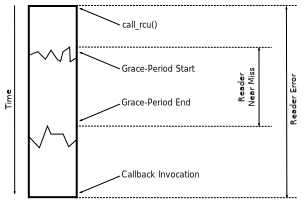
\includegraphics{debugging/RCUnearMiss}}
\caption{RCU Errors and Near Misses}
\label{fig:debugging:RCU Errors and Near Misses}
\end{figure}

예를 들어, RCU 의 우선순위 올리기에 있는 낮은 확률의 버그는 rcutorture 의
집중된 테스트에서 대략 100 시간에 한번 일어났습니다.
그 버그가 일어날 확률이 상당히 감소되었음을 99\,\% 확신하기 위해서는 거의 500
시간의 실패 없는 테스트 수행이 필요하기 때문에, 그 실패를 찾아내기 위한 \co{git
bisect} 과정은 고통스러울 정도로 느릴겁니다---또는 극단적으로 거대한 테스트
환경을 필요로 할겁니다.
다행히도, 테스트된 해당 RCU 오퍼레이션은 RCU grace period 를 위한 대기만이
아니라, 시작하기 위한 그 grace period 에 대한 앞선 대기와 그 RCU grace period
가 완료된 후에 호출될 RCU callback 을 위한 뒤이은 대기도 존재했습니다.
\co{rcutorture} 에러와 near miss 사이의 차이가
Figure~\ref{fig:debugging:RCU Errors and Near Misses} 에 보여져 있습니다.
완전히 본격적인 에러로 구분되기 위해서, RCU read-side 크리티컬 섹션은 grace
period 를 시작한 \co{call_rcu()} 로부터 앞의 grace period 의 남아있는 부분과
\co{call_rcu()} 로 시작된 grace period 전체 (지그재그로 그어진 선으로 표시된
영역), 그리고 그 grace period 의 끝으로부터 callback 의 호출 사이의 딜레이까지
확장되는데, 이게 ``Error'' 화살표로 표시되어 있습니다.
\iffalse

For example, a low-probability bug in RCU priority boosting occurred
roughly once every hundred hours of focused rcutorture testing.
Because it would take almost 500 hours of failure-free testing to be
99\,\% certain that the bug's probability had been significantly reduced,
the \co{git bisect} process
to find the failure would be painfully slow---or would require an extremely
large test farm.
Fortunately, the RCU operation being tested included not only a wait for
an RCU grace period, but also a previous wait for the grace period to start
and a subsequent wait for an RCU callback to be
invoked after completion of the RCU grace period.
This distinction between an \co{rcutorture} error and near miss is
shown in
Figure~\ref{fig:debugging:RCU Errors and Near Misses}.
To qualify as a full-fledged error, an RCU read-side critical section
must extend from the \co{call_rcu()} that initiated a grace period,
through the remainder of the previous grace period, through the
entirety of the grace period initiated by the \co{call_rcu()}
(denoted by the region between the jagged lines), and
through the delay from the end of that grace period to the callback
invocation, as indicated by the ``Error'' arrow.
\fi
하지만, 정식적인 RCU 의 정의는 RCU read-side 크리티컬 섹션이 하나의 grace
period 사이로 확장되는 것을 금지하는데, 이는 ``Near Miss'' 화살표로 나타내어져
있습니다.
이는 near miss 들을 에러 조건으로 사용할 것을 제안하지만, 다른 CPU 들은 해당
grace period 가 정확히 언제 시작되고 종료되었는지에 대해 지그재그로 그어진
선으로 보여지듯이 다른 의견을 가질 수 있기 때문에, 이는 문제가 될 수
있습니다.\footnote{
	아무일도 하지 않고 있는 CPU 들은 최근의 수백개의 grace period들에
	대해서도 전혀 알지 못하고 있을 수도 있기 때문에, 이 지그재그로 그어진
	라인들은 상당히 과소평가 되어 있습니다.}
따라서 이 near miss 들을 에러 컨디션으로 사용하는 것은 거짓 양성 결과를
만들어낼 수 있는데, 이는 자동화된 \co{rcutorture} 테스트에서는 제거되어야
합니다.
\iffalse

However, the formal definition of RCU prohibits RCU read-side critical
sections from extending across a single grace period, as indicated by
the ``Near Miss'' arrow.
This suggests using near misses as the error condition, however, this
can be problematic because different CPUs can have different opinions
as to exactly where a given
grace period starts and ends, as indicated by the jagged lines.\footnote{
	The jaggedness of these lines is seriously understated because
	idle CPUs might well be completely unaware of the most recent
	few hundred grace periods.}
Using the near misses as the error condition could therefore result
in false positives, which need to be avoided in the automated
\co{rcutorture} testing.
\fi

순수히 바보같은 운으로 인해, \co{rcutorture} 는 grace period 의 near-miss
버전에 민감한 통계를 포함하게 되었습니다.
앞서 이야기한대로, 이런 통계들은 RCU 의 상태 변수들에 대한 동기화 되지 않은
액세스로 인해서 거짓 양성 결과에 영향을 받기 쉽습니다만, 이런 거짓 양성 결과는
IBM 메인프레임이나 x86 과 같은 강한 순서 규칙의 시스템들에서는 상당히 희귀하게
발생하는 것으로 드러났는데, 1000 시간의 테스트 가운데 한번 보다도 낮은 확률로
일어납니다.

이런 near miss 들은 대략 한시간에 한번 꼴로 발생했는데, 이는 실제 에러들보다
100배 이상 빈번하게 발생하는 겁니다.
이런 near miss 들의 사용은 버그의 원인을 일주일 안되는 시간 내에 파악해내고
수정된 내용의 효과를 하루 내에 확신하는 것을 가능하게 했습니다.
반면에, 진짜 에러만을 보기 위해서 near miss 들을 제외시키는 행위는 수개월의
디버그와 검증 시간을 필요로 했습니다.
\iffalse

By sheer dumb luck, \co{rcutorture} happens to include some statistics that
are sensitive to the near-miss version of the grace period.
As noted above, these statistics are subject to false positives due to
their unsynchronized access to RCU's state variables,
but these false positives turn out to be extremely rare on strongly
ordered systems such as the IBM mainframe and x86, occurring less than
once per thousand hours of testing.

These near misses occurred roughly once per hour, about two orders of
magnitude more frequently than the actual errors.
Use of these near misses allowed the bug's root cause to be identified
in less than a week and a high degree of confidence in the fix to be
built in less than a day.
In contrast, excluding the near misses in favor of the real errors would
have required months of debug and validation time.
\fi

Near-miss 카운팅을 정리하자면, 일반적인 방법은 빈번하지 않게 발생하는 실패의
횟수를 세는 것을 더 빈번하게 발생하며 그 실패들과 연과노디어 있을 것으로
여겨지는 near miss 의 횟수를 세는 것으로 대체하는 것입니다.
이런 near-miss 들은 진짜 실패의 heisenbug 에 대한 anti-heisenbug 로 여겨질 수
있는데, 더 빈번하게 발생하는 near-miss 들은 예를 들어 디버깅 코드를 추가하기
위해 만드는 것과 같은 코드의 변경이 있는 상황에서도 그 발생률이 더 일관될
것이기 때문입니다.

여태까지, 우리는 병렬 프로그램의 기능성에서의 버그들에 대해서만 집중해
왔습니다.
하지만, 성능이 병렬 프로그램에서의 첫번째 필요사항이기 때문에 (그렇지 않다면,
순차적 프로그램을 짜지 그러세요?), 다음 섹션에서는 성능상의 버그들을 찾아내는
방법을 알아봅니다.
\iffalse

To sum up near-miss counting, the general approach is to replace counting
of infrequent failures with more-frequent near misses that are believed
to be correlated with those failures.
These near-misses can be considered an anti-heisenbug to the real failure's
heisenbug because the near-misses, being more frequent, are likely to
be more robust in the face of changes to your code, for example, the
changes you make to add debugging code.
\fi

\subsubsection{Heisenbug Discussion}
\label{sec:debugging:Heisenbug Discussion}

주의깊은 독자라면 이 섹션이
Section~\ref{sec:debugging:Statistics for Discrete Testing},
~\ref{sec:debugging:Abusing Statistics for Discrete Testing},
그리고~\ref{sec:debuggingStatistics for Continuous Testing} 의 정교한 수학에
비해 모호하고 계량적임을 눈치챘을 겁니다.
여러분이 정확성과 수학을 사랑한다면, 이 섹션이 적용될 수 있는 환경이 앞의
섹션들이 적용될 수 있는 것에 비해 상당히 더 흔하다는 사실에 실망할 수도 있을
겁니다.
\iffalse

The alert reader might have noticed that this section was fuzzy and
qualitative, in stark contrast to the precise mathematics of
Sections~\ref{sec:debugging:Statistics for Discrete Testing},
~\ref{sec:debugging:Abusing Statistics for Discrete Testing},
and~\ref{sec:debuggingStatistics for Continuous Testing}.
If you love precision and mathematics, you may be disappointed to
learn that the situations to which this section applies are far
more common than those to which the preceding sections apply.
\fi

여러분의 코드에 버그가 있을 것이라 믿는다 해도, 그 버그들이 무엇인지, 무엇이
그것을 일으켰는지, 그것들이 어떻게 나타날 것인지, 또는 어떤 조건이 그것들의
발생 확률에 영향을 끼치는지를 알 수 없다는게 실제로 그 흔한 상황입니다.
이 모든-너무-흔한 경우에, 통계는 여러분을 돕지 못합니다.\footnote{
	여러분의 프로그램이 (여러분 생각과 달리 그럴 확률이 적겠지만) 해야 할
	일이 무엇인지 알고 여러분의 프로그램이 충분히 작다면
	Chapter~\ref{chp:Formal Verification} 에서 설명한 정적 검증 도구가
	도움이 될 수 있긴 합니다.}
바꿔 말하면, 통계가 여러분을 \emph{직접적으로} 돕지는 못합니다.
하지만 통계는 간접적인 커다란 도움을 줄 수 있는데---\emph{만약} 여러분이 (예를
들면, 충분히 sleep 을 해버린다던가 함으로써) 실수의 확률을 줄일 수도 있는
실수를 만들 수 있다는걸 인정하는데 필요한, 그리고 여러분이 과거에 만들어낸
실수들의 수와 종류가 미래에도 일어날 수 있다는걸 인정하는데 필요한 겸손을
갖는다면 그렇습니다.
예를 들어, 저는 초기화 코드의 작지만 치명적인 부분들을 작성하는 걸 잊고 종종
병렬 프로그램의 정확성의 대부분 또는 전체를 망가뜨리는 개탄스러운 성향을 갖고
있습니다.
일단 제가 이런 종류의 실수에 취약하다는 사실을 스스로 인정하려 한 것은, 저
자신이 제 초기화 코드를 두번씩 체크하도록 하는걸 더 쉽게 (하지만 쉽지 않아요!)
해줬습니다.
이렇게 하는게 제가 많은 버그들을 찾을 수 있게 해줬습니다.
\iffalse

In fact, the common case is that although you might have reason to believe
that your code has bugs, you have no idea what those bugs are, what
causes them, how likely they are to appear, or what conditions affect
their probability of appearance.
In this all-too-common case, statistics cannot help you.\footnote{
	Although if you know what your program is supposed to do and
	if your program is small enough (both less likely that you
	might think), then the formal-verification tools described in
	Chapter~\ref{chp:Formal Verification}
	can be helpful.}
That is to say, statistics cannot help you \emph{directly}.
But statistics can be of great indirect help---\emph{if} you have the
humility required to admit that you make mistakes, that you can reduce the
probability of these mistakes (for example, by getting enough sleep), and
that the number and type of mistakes you made in the past is indicative of
the number and type of mistakes that you are likely to make in the future.
For example, I have a deplorable tendency to forget to write a small
but critical portion of the initialization code, and frequently get most
or even all of a parallel program correct---except for a stupid
omission in initialization.
Once I was willing to admit to myself that I am prone to this type of
mistake, it was easier (but not easy!) to force myself to double-check
my initialization code.
Doing this allowed me to find numerous bugs ahead of time.
\fi

Taleb 의 명명법~\cite{NassimTaleb2007BlackSwan} 을 사용하면, white swan 은
우리가 재현할 수 있는 버그입니다.
우린 더 많은 수의 테스트를 수행하고, 그 버그의 확률을 추정하는데 보통의 통계를
사용하고, 우리의 수정 여부 신뢰성을 추정하는데 보통의 통계를 사용할 수
있습니다.
예상치 못한 버그는 black swan 입니다.
우린 그에 대해 아무것도 알지 못하고, 그걸 발생시킬 수 있는 테스트를 가지고 있지
않으며, 통계도 도움이 되지 못합니다.
우리 스스로의 행동을 연구하는 것, 특히 우리가 만들어내는 실수들의 수와 종류를
연구하는 것은 black swan 들을 grey swan 으로 바꿔 놓을 수 있습니다.
일반적인 통계는 (우리가 이 버그들을 재현할 수 있게 되기 전까지는) 여전히 도움이
되지 않을 뿐더러 취약합니다\footnote{
	바꿔말하면 악독합니다.}
테스트 방법론들은 큰 도움이 될 수 있습니다.
따라서, 목표는 이 black swan 들을 grey swan 들로 바꾸는 경험과 좋은 검증
방법들을 사용하고, 이 grey swan 들을 white swan 들로 바꾸기 위해 집중된
테스트와 분석을 사용하고, 이 white swan 들을 고치는데 일반적 방법들을 사용하는
것입니다.
\iffalse

Using Taleb's nomenclature~\cite{NassimTaleb2007BlackSwan},
a white swan is a bug that we can reproduce.
We can run a large number of tests, use ordinary statistics to
estimate the bug's probability, and use ordinary statistics again
to estimate our confidence in a proposed fix.
An unsuspected bug is a black swan.
We know nothing about it, we have no tests that have yet caused it
to happen, and statistics is of no help.
Studying our own behavior, especially the number and types of mistakes
we make, can turn black swans into grey swans.
We might not know exactly what the bugs are, but we have some idea of
their number and maybe also of their type.
Ordinary statistics is still of no help (at least not until we are
able to reproduce one of the bugs), but robust\footnote{
	That is to say brutal.}
testing methods can be of great help.
The goal, therefore, is to use experience and good validation practices
to turn the black swans grey, focused testing and analysis to turn the
grey swans white, and ordinary methods to fix the white swans.
\fi

그렇다고는 하나, 우린 병렬 프로그램의 기능성에 대한 버그에만 집중해 왔습니다.
하지만, 성능이야말로 병렬 프로그램의 1급 필요성이기 때문에 (아니라면, 순차적
프로그램을 써야겠죠?), 다음 섹션에서는 성능 버그에 대해 이야기 하겠습니다.
\iffalse

That said, thus far, we have focused solely on bugs in the parallel program's
functionality.
However, because performance is a first-class requirement for a
parallel program (otherwise, why not write a sequential program?),
the next section discusses performance bugs.
\fi

\section{Performance Estimation}
\label{sec:debugging:Performance Estimation}
%
\epigraph{There are lies, damn lies, statistics, and benchmarks.}
	 {\emph{Unknown}}

병렬 프로그램은 보통 성능과 확장성에 대한 요구를 받게 됩니다, 무엇보다, 만약
성능이 문제가 아니라면, 순차적 프로그램을 사용하는게 낫겠죠?
궁극의 성능과 선형적 확장성은 필요치 않을 수도 있습니다만, 순차적으로 같은 일을
하는 최적화된 프로그램보다 느리게 동작하는 병렬 프로그램은 많이 사용되지 않을
겁니다.
그리고 마이크로세컨드도 문제가 되고 나노세컨드라도 필요한 경우들이 정말로
존재합니다.
따라서, 병렬 프로그램에 있어서, 불충분한 성능은 올바르지 못하게 동작하는
것만큼이나 커다란 버그입니다.
\iffalse

Parallel programs usually have performance and scalability requirements,
after all, if performance is not an issue, why not use a sequential
program?
Ultimate performance and linear scalability might not be necessary, but
there is little use for a parallel program that runs slower than its
optimal sequential counterpart.
And there really are cases where every microsecond matters and every
nanosecond is needed.
Therefore, for parallel programs, insufficient performance is just as
much a bug as is incorrectness.
\fi

\QuickQuiz{}
	그건 웃긴 이야기네요!!!
	어쨌든, 좀 늦더라도 올바른 답을 얻는게 잘못된 답을 얻는 것보다는 낫지
	않겠어요???
	\iffalse

	That is ridiculous!!!
	After all, isn't getting the correct answer later than one would like
	better than getting an incorrect answer???
	\fi
\QuickQuizAnswer{
	이 질문은 아예 답을 계산하지 않는, 그리고 그렇게 함으로써, 또한 그 답을
	계산하는데 드는 비용을 고려하게 만드는 선택지를 고려하게 만듭니다.
	예를 들어, 짧은 기간의 날씨 예측과 같은, 정확한 모델들이 존재하지만
	정말로 그 날씨가 와버리기보다 먼저 그 모델을 수행하기를 원한다면 커다란
	(그리고 비싼) 클러스터로 구성된 슈퍼컴퓨터들을 필요로 하는 경우를
	생각해 보세요.
	\iffalse

	This question fails to consider the option of choosing not to
	compute the answer at all, and in doing so, also fails to consider
	the costs of computing the answer.
	For example, consider short-term weather forecasting, for which
	accurate models exist, but which require large (and expensive)
	clustered supercomputers, at least if you want to actually run
	the model faster than the weather.
	\fi

	그리고 이 경우에, 그 모델이 실제 날씨보다 빠르게수행되는 것을 방지하는
	모든 성능 버그는 모든 날씨 예측을 방지해 버립니다.
	그 커다란 클러스터로 구성된 슈퍼컴퓨터들을 구입한 목적은 모두 날씨를
	예측하기 위해서였다는 점을 생각해 보면, 그 모델을 날씨보다 빠르게
	수행하지 못한다면, 그 모델을 아예 수행하지 않는 편이 나을 겁니다.

	안전성에 민감한 리얼타임 컴퓨팅 분야에서는 더 많은 가혹한 예들이 발견될
	수도 있을 겁니다.
	\iffalse

	And in this case, any performance bug that prevents the model from
	running faster than the actual weather prevents any forecasting.
	Given that the whole purpose of purchasing the large clustered
	supercomputers was to forecast weather, if you cannot run the
	model faster than the weather, you would be better off not running
	the model at all.

	More severe examples may be found in the area of safety-critical
	real-time computing.
	\fi
} \QuickQuizEnd

\QuickQuiz{}
	하지만, 어플리케이션을 병렬화하기 위해 필요한 모든 어려운 일을 해내기로
	했다면 왜 그걸 올바르게 하지 않는거죠?
	왜 최적의 성능과 선형적인 확장성보다 못한 것에 안주하는 겁니까?
	\iffalse

	But if you are going to put in all the hard work of parallelizing
	an application, why not do it right?
	Why settle for anything less than optimal performance and
	linear scalability?
	\fi
\QuickQuizAnswer{
	전 정말로 당신의 정신과 포부에 경의를 표합니다만, 당신은 프로그램의
	완료에 걸리는 딜레이가 높은 비용이 될수도 있다는 점을 잊고 있습니다.
	극단적인 예를 들어보면, 단일 쓰레드로 짜인 어플리케이션에서의 40\,\% 의
	성능 저하가 매일 한 사람을 죽게 만든다고 생각해 보세요.
	더 나아가서 당신이 사람들과 함께 여덟게의 CPU 를 가진 시스템에서 순차적
	버전에 비해서 50\,\% 빠르게 동작하는 병렬 프로그램을 하루만에 빠르고
	지저분하게 만들어 냈지만(hack), 최적의 병렬 프로그램은 네달동안의
	고통스러운 설계, 코딩, 디버깅, 그리고 최적화를 필요로 한다고 상상해
	보세요.

	백명이 넘는 사람들은 그 빠르고 더럽게 만들어진 버전을 더 좋아할 거라고
	충분히 말할 수 있습니다.
	\iffalse

	Although I do heartily salute your spirit and aspirations,
	you are forgetting that there may be high costs due to delays
	in the program's completion.
	For an extreme example, suppose that a 40\,\% performance shortfall
	from a single-threaded application is causing one person to die
	each day.
	Suppose further that in a day you could hack together a
	quick and dirty
	parallel program that ran 50\,\% faster on an eight-CPU system
	than the sequential version, but that an optimal parallel
	program would require four months of painstaking design, coding,
	debugging, and tuning.

	It is safe to say that more than 100 people would prefer the
	quick and dirty version.
	\fi
} \QuickQuizEnd

따라서 병렬 프로그램을 검증하는 일은 그 성능을 검증하는 것을 포함합니다.
하지만 성능을 검증하는 일은 수행시킬 워크로드와 그 프로그램을 평가할 성능
지표를 가지고 있음을 의미합니다.
이런 필요한 것들은 \emph{성능 벤치마크}로 얻어지기도 하는데, 다음 섹션에서 이에
대해 논해 봅니다.
\iffalse

Validating a parallel program must therfore include validating its
performance.
But validating performance means having a workload to run and performance
criteria with which to evaluate the program at hand.
These needs are often met by \emph{performance benchmarks}, which
are discussed in the next section.
\fi

\subsection{Benchmarking}
\label{sec:debugging:Benchmarking}

오래된 말로 ``거짓말이 있어, 빌어먹을 거짓말, 통계, 그리고 벤치마크들.'' 란
말이 있죠.
하지만, 벤치마크들은 상당히 많이 사용되고 있고, 따라서 그것들을 지나치게
멸시하는 것은 도움이 되지 않습니다.

벤치마크들은 임시 변통의 움직임들부터 국제적인 표준까지 그 범위가 다양합니다만,
그것들의 정형성의 수준과는 관계없이, 벤치마크들은 네개의 주요 목적을
처리합니다:
\iffalse

% TODO: Apply
Frequent abuse aside, benchmarks are both useful and heavily used,
so it is not helpful to be too dismissive of them.
Benchmarks span the range from ad hoc test jigs to international
standards, but regardless of their level of formality, benchmarks
serve four major purposes:
\fi

\begin{enumerate}
\item	비교되는 구현들을 공정하게 비교하기 위한 프레임웍을 제공합니다.
\item	사용자에게 가치있는 방향으로 구현을 개선하기 위한 경쟁적 에너지에
	집중합니다.
\item	벤치마크되는 구현의 예제적 사용으로서의 역할을 합니다.
\item	당신의 소프트웨어의 강점을 경쟁자가 제공하는 것에 대비해서 강조하는
	마케팅 도구의 역할을 합니다.
\iffalse

\item	Providing a fair framework for comparing competing implementations.
\item	Focusing competitive energy on improving implementations in ways
	that matter to users.
\item	Serving as example uses of the implementations being benchmarked.
% TODO: Apply
\item	Serving as a marketing tool to highlight your software
	against your competitors' offerings.
\end{enumerate}

물론, 완전하게 공정한 프레임웍은 의도된 어플리케이션 그 자체밖에 없습니다.
그런데 벤치마킹에서의 공정성에 대해서 신경쓰는 사람이라면 단순히 그
어플리케이션 자체를 벤치마크로 사용하는 대신에 불완전한 벤치마크들을 만들어낼
생각을 하는 걸까요?

실제 어플리케이션을 수행하는 것은 그게 실용적인 곳에서라면 실제로 그게 최고의
방법입니다.
불행히도, 그건 다음과 같인 이유로 실용적이지 못한 경우가 많습니다:
\iffalse

Of course,  the only completely fair framework is the intended
application itself.
So why would anyone who cared about fairness in benchmarking
bother creating imperfect benchmarks rather than simply
using the application itself as the benchmark?

Running the actual application is in fact the best approach where it is practical.
Unfortunately, it is often impractical for the following reasons:
\fi

\begin{enumerate}
\item	그 어플리케이션은 독점된 것이고, 당신이 그 의도된 어플리케이션을 수행할
	권한을 갖고 있지 못할 수 있습니다.
\item	그 어플리케이션은 당신이 접근할 수 없는 더 많은 하드웨어를 필요로 할
	수도 있습니다.
\item	그 어플리케이션은 당신이 예를 들어 개인정보 규제와 같은 이유로 법적으로
	접근할 수 없는 데이터를 사용할 수도 있습니다.
\iffalse

\item	The application might be proprietary, and you
	might not have the right to run the intended application.
\item	The application might require more hardware
	than you have access to.
\item	The application might use data that you cannot
	access, for example, due to privacy regulations.
\fi
\end{enumerate}

이런 경우에, 그 어플리케이션을 모사하는 벤치마크를 반드는 것이 이런 문제들을
극복하는데 도움이 될 수 있습니다.
세심하게 구성된 벤치마크는 성능, 확장성, 에너지 효율성, 그리고 그 외에도 많은
것들을 촉진시키는데 도움이 될 수 있습니다.
\iffalse

% TODO: Apply
Creating a benchmark that approximates
the application can help overcome these obstacles.
A carefully constructed benchmark can help promote performance,
scalability, energy efficiency, and much else besides.
However, be careful to avoid investing too much into the benchmark
effort.
It is after all important to invest at least a little into the
application itself~\cite{Gray91}.
\fi

\subsection{Profiling}
\label{sec:debugging:Profiling}

소프트웨어의 매우 작은 부분이 성능과 확장성 한계의 주요한 책임을 가지고 있는
경우가 많습니다.
하지만, 개발자들이 실제 병목지점을 손으로 찾아내기는 악명높도록 불가능합니다.
예를 들어, 커널 버퍼 할당자의 경우에 있어서, 모든 관심은 밀집도가 높은 배열의
탐색에 집중되었습니다만 이는 할당자의 실행 시간 중 몇 퍼센트만을 차지하는
것으로 드러났습니다.
논리 분석기를 통해 수집된 수행 프로파일은 정말로 문제의 주요한 부분에 책임이
있었던 캐시 미스에 관심을 집중시켰습니다~\cite{McKenney93}.

성능과 확장성 버그를 추적하는데 있어 옛날 방식이지만 상당히 효과적인 한가지
방법은 프로그램을 디버거와 물려서 수행시키면서 주기적으로 프로그램을 인터럽트
하고서 매 인터럽트마다 모든 쓰레드의 스택을 기록하는 것입니다.
여기서의 이론은 무언가가 프로그램을 느리게 만들고 있다면, 그것은 쓰레드의
수행에 보일 것이라는 것입니다.
\iffalse

In many cases, a fairly small portion of your software is responsible
for the majority of the performance and scalability shortfall.
However, developers are notoriously unable to identify the actual
bottlenecks by hand.
For example, in the case of a kernel buffer allocator, all attention focused
on a search of a dense array which turned out to represent only
a few percent of the allocator's execution time.
An execution profile collected via a logic analyzer focused attention
on the cache misses that were actually responsible for the majority
of the problem~\cite{McKenney93}.

An old-school but quite effective method of tracking down performance
and scalability bugs is to run your program under a debugger,
then periodically interrupt it, recording the stacks of all threads
at each interruption.
The theory here is that if something is slowing down your program,
it has to be visible in your threads' executions.
\fi

그렇다곤 하지만, 당신의 관심을 가장 필요한 곳에 집중할 수 있도록 도와주는데
있어 일반적으로는 훨씬 나은 일을 해주는 많은 도구들이 있습니다.
대중적인 두가지 선택이 있는데 \co{gprof} 와 \co{perf} 입니다.
단일 프로세스 프로그램에 \co{perf} 를 사용하려 한다면 그 프로그램을 수행하는
커맨드 앞에 \co{perf record} 를 붙여서 수행하고, 그 커맨드가 완료된 후에,
\co{perf report} 를 입력하세요.
멀티 쓰레드 프로그램의 성능 디버깅을 위한 도구를 위한 수많은 작업들이 있었는데,
이것들은 이 중요한 일을 좀 더 쉽게 만들었습니다.
다시한번 말하지만, Brendan Gregg 의 블로그가 시작점으로 좋습니다.\footnote{
	\url{http://www.brendangregg.com/blog/}}
\iffalse

That said, there are a number of tools
that will usually do a much better job of helping you to focus your
attention where it will do the most good.
Two popular choices are \co{gprof} and \co{perf}.
To use \co{perf} on a single-process program, prefix your command
with \co{perf record}, then after the command completes, type
\co{perf report}.
There is a lot of work on tools for performance debugging of multi-threaded
programs, which should make this important job easier.
Again, one good starting point is Brendan Gregg's blog.\footnote{
	\url{http://www.brendangregg.com/blog/}}
\fi

\subsection{Differential Profiling}
\label{sec:debugging:Differential Profiling}

확장성 문제는 프로그램을 매우 큰 시스템들에서 수행해보기 전까지는 분명하지 않을
겁니다.
하지만, 훨씬 작은 시스템들에서 프로글매을 수행할 때라고 해도 임박한 확장성
문제들을 찾아내는 것이 가능할 때도 있습니다.
이를 위한 한가지 테크닉은 \emph{차이점 프로파일링 (differential profiling)}
이라고 불립니다.

아이디어는 워크로드를 두개의 서로 다른 조건들의 집합에서 수행해 보는 겁니다.
예를들어, 워크로드를 두개의 CPU 위에서 돌려볼 수 있고, 그러고나서는 또다시
네개의 CPU 위에서 해보는 겁니다.
또는 시스템에 가하는 부하의 정도, 네트워크 어댑터들의 갯수, 대용량 저장장치의
갯수, 등등을 다양하게 변화시켜볼 수 있습니다.
그러고나선 두 수행의 프로파일들을 모으고, 수학적으로 관련된 프로파일 측정결과를
조합해 보는 겁니다.
예를 들어, 주요한 관심이 확장성이라면, 연관된 측정의 비율을 취하고, 그 비율들을
숫자상으로 내림차순으로 정렬해 볼 수 있을 겁니다.
가장 의심스러운 확장성에 대한 용의자는 정렬된 리스트의 꼭대기에 위치하게
될겁니다~\cite{McKenney95a,McKenney99b}.

\co{perf} 와 같은 일부 도구들은 내장된 차이점 프로파일링 지원 기능을 가지고
있습니다.
\iffalse

Scalability problems will not necessarily be apparent unless you are running
on very large systems.
However, it is sometimes possible to detect impending scalability problems
even when running on much smaller systems.
One technique for doing this is called \emph{differential profiling}.

The idea is to run your workload under two different sets of conditions.
For example, you might run it on two CPUs, then run it again on four
CPUs.
You might instead vary the load placed on the system, the number of
network adapters, the number of mass-storage devices, and so on.
You then collect profiles of the two runs, and mathematically combine
corresponding profile measurements.
For example, if your main concern is scalability, you might take the
ratio of corresponding measurements, and then sort the ratios into
descending numerical order.
The prime scalability suspects will then be sorted to the top of the
list~\cite{McKenney95a,McKenney99b}.

Some tools such as \co{perf} have built-in differential-profiling
support.
\fi

\subsection{Microbenchmarking}
\label{sec:debugging:Microbenchmarking}

마이크로벤치마킹은 소프트웨어의 더 큰 부분에 포함되기에 어떤 알고리즘이나
데이터 구조가 더 적합할지를 결정하는데에 있어 더 깊은 평가를 위해 유용할 수
있습니다.

마이크로 벤치마킹을 하는 흔한 방법 한가지는 시각을 측정하고, 테스트 되는 코드를
몇번 반복해서 수행시키고, 다시 시각을 측정하는 것입니다.
두개의 시각 사이의 차이를 반복 횟수로 나누면 테스트 되는 코드를 수행하는데
필요한 시간의 측정값이 나옵니다.

불행히도, 측정을 위한 이 방법은 여러개의 에러가 끼어들 수 있게 하는데, 다음과
같은 것들이 있습니다:
\iffalse

Microbenchmarking can be useful when deciding which algorithms or
data structures are worth incorporating into a larger body of software
for deeper evaluation.

One common approach to microbenchmarking is to measure the time,
run some number of iterations of the code
under test, then measure the time again.
The difference between the two times divided by the number of iterations
gives the measured time required to execute the code under test.

Unfortunately, this approach to measurement allows any number of errors
to creep in, including:
\fi

\begin{enumerate}
\item	이 측정은 시각 측정의 오버헤드가 포함될 수 있습니다.
	이런 에러는 수행 반복 횟수를 증가시킴으로써 임의의 작은 값으로 줄일 수
	있습니다.
\item	처음 몇번의 테스트 수행 반복은 캐시 미스나 (더 나쁜) 페이지 폴트를
	유발할 수도 있는데, 이는 측정된 값을 부풀릴 수도 있을 겁니다.
	이런 에러는 역시 수행 반복의 수를 늘림으로써 줄일 수 있으며, 측정
	기간이 시작되기 전에 몇번의 웜업 수행 반복을 수행시킴으로써 완전히
	없앨수 있는 경우도 많습니다.
\item	예를 들어 임의의 메모리 에러와 같은 간섭의 일부 종류들은 테스트의 수행
	반복의 여러 세트를 수행시킴으로써 조치가 될 수 있을 정도로 드물게
	발생합니다.
	만약 간섭의 정도가 통계적으로 심각하다면, 모든 유난스럽게 다른 성능
	결과들을 통계적으로 제거시킬 수 있습니다.
\iffalse

\item	The measurement will include some of the overhead of
	the time measurement.
	This source of error can be reduced to an arbitrarily small
	value by increasing the number of iterations.
\item	The first few iterations of the test might incur cache misses
	or (worse yet) page faults that might inflate the measured
	value.
	This source of error can also be reduced by increasing the
	number of iterations, or it can often be eliminated entirely
	by running a few warm-up iterations before starting the
	measurement period.
\item	Some types of interference, for example, random memory errors,
	are so rare that they can be dealt with by running a number
	of sets of iterations of the test.
	If the level of interference was statistically significant,
	any performance outliers could be rejected statistically.
\fi
\item	모든 테스트 반복 수행이 시스템의 다른 활동에 의해 간섭을 받을 수
	있습니다.
	간섭의 근원은 다른 어플리케이션들, 시스템 유틸리티들과 데몬, 디바이스
	인터럽트, 펌웨어 인터럽트 (시스템 관리 인터럽트인 SMI 포함), 가상화,
	메모리 에러, 그리고 그 외에도 다른 여러가지가 있을 수 있습니다.
	이런 간섭 유발사건들이 무작위적으로 발생한다고 가정하면, 그것들의
	효과는 반복 횟수를 줄임으로써 최소화 시킬 수 있습니다.
\iffalse

\item	Any iteration of the test might be interfered with by other
	activity on the system.
	Sources of interference include other applications, system
	utilities and daemons, device interrupts, firmware interrupts
	(including system management interrupts, or SMIs),
	virtualization, memory errors, and much else besides.
	Assuming that these sources of interference occur randomly,
	their effect can be minimized by reducing the number of
	iterations.
\fi
\end{enumerate}

간섭 유발 사건들 중 첫번째와 네번째 것은 서로 상충되는 조언을 하고 있는데, 이건
우리가 실제 세계에 살고 있다는 한가지 증거입니다.
이 섹션의 나머지 부분에서는 이런 상충되는 것을 어떻게 해결해야 할지 알아봅니다.
\iffalse

The first and fourth sources of interference provide conflicting advice,
which is one sign that we are living in the real world.
The remainder of this section looks at ways of resolving this conflict.
\fi

\QuickQuiz{}
	하지만, 예를 들어 캐시와 메모리 배치 사이의 간섭에 의한 것과 같은 다른
	에러 유발 원인들은 어떻게 하죠?
	\iffalse

	But what about other sources of error, for example, due to
	interactions between caches and memory layout?
	\fi
\QuickQuizAnswer{
	메모리 배치의 변경은 실제로 비현실적으로 수행 시간을 줄여버리는 결과를
	초래할 수 있습니다.
	예를 들어, 어떤 마이크로벤치마크는 거의 항상 L0 캐시의 associativity 를
	오버플로우 시키지만, 올바른 메모리 배치에서만큼은 모두 맞아떨어진다고
	생각해보세요.
	이게 정말 문제라면, 메모리 배치를 완전히 제어할 수 있도록
	마이크로벤치마크를 huge page 를 사용해서 수행해보는 방안 (또는 커널에서
	수행하거나 기계 위에서 곧바로)을 생각해 보세요.
	\iffalse

	Changes in memory layout can indeed result in unrealistic
	decreases in execution time.
	For example, suppose that a given microbenchmark almost
	always overflows the L0 cache's associativity, but with just the right
	memory layout, it all fits.
	If this is a real concern, consider running your microbenchmark
	using huge pages (or within the kernel or on bare metal) in
	order to completely control the memory layout.
	\fi
} \QuickQuizEnd

다음의 섹션들은 측정 에러들을 처리하는 방법들을 이야기 해보는데,
Section~\ref{sec:debugging:Isolation} 에서는 일부 형태의 간섭들을 막기 위해서
사용될 수 있는 격리화 테크닉들을 다루고,
Section~\ref{sec:debugging:Detecting Interference} 는 간섭으로 인해 오염되었을
수 있는 측정 데이터를 버릴 수 있도록 간섭을 파악하는 방법들을 다룹니다.
\iffalse

The following sections discuss ways of dealing with these measurement
errors, with
Section~\ref{sec:debugging:Isolation}
covering isolation techniques that may be used to prevent some forms of
interference,
and with
Section~\ref{sec:debugging:Detecting Interference}
covering methods for detecting interference so as to reject measurement
data that might have been corrupted by that interference.
\fi

\subsection{Isolation}
\label{sec:debugging:Isolation}

리눅스 커널은 특정 CPU 들을 바깥의 간섭으로부터 격리시키는 몇가지 방법들을
제공합니다.

먼저, 다른 프로세스, 쓰레드, 그리고 태스크들에 의해 가해질 수 있는 간섭을
봅시다.
POSIX \co{sched_setaffinity()} 시스템 콜은 많은 태스크들을 특정 CPU 들로부터
몰아내고 당신의 테스트들을 같은 그룹의 CPU 들로 가둬두는데 사용될 수 있습니다.
리눅스에 존재하는 사용자 레벨 \co{taskset} 커맨드도 같은 목적으로 사용될 수도
있습니다만 \co{sched_setaffinity()} 와 \co{taskset} 은 모두 상승되는 권한을
필요로 하긴 합니다.
리눅스에 존재하는 control groups (cgroups) 가 같은 목적으로 사용될 수도
있습니다.
이 방법은 간섭을 줄이는데 있어 상당히 효과적일 수 있고, 많은 경우에는 이걸로
충분합니다.
하지만, 이 방법도 한계가 있는데, 예를 들어, 태스크들을 잡아두기 위해 자주
사용되는 per-CPU 커널 쓰레드들에 대해서는 아무일도 해주지 못합니다.
\iffalse

The Linux kernel provides a number of ways to isolate a group of
CPUs from outside interference.

First, let's look at interference by other processes, threads, and tasks.
The POSIX \co{sched_setaffinity()} system call may be used to move
most tasks off of a given set of CPUs and to confine your tests to
that same group.
The Linux-specific user-level \co{taskset} command may be used for
the same purpose, though both \co{sched_setaffinity()} and
\co{taskset} require elevated permissions.
Linux-specific control groups (cgroups) may be used for this same purpose.
This approach can be quite effective at reducing interference, and
is sufficient in many cases.
However, it does have limitations, for example, it cannot do anything
about the per-CPU kernel threads that are often used for housekeeping
tasks.
\fi

per-CPU 커널 쓰레드들로부터의 간섭을 피하는 한가지 방법은, 예를 들어 POSIX
\co{sched_Setscheduler()} 시스템 콜을 이용하거나 해서 테스트를 높은 real-time
우선순위로 수행시키는 것입니다.
하지만, 만약 이렇게 할 경우, 당신은 묵시적으로 무한 루프를 막는다는 책임을 갖게
되는 것인데, 그러지 않는다면 그 테스트는 커널의 한 부분이 동작을 못하게 만들어
버릴 것이기 때문입니다.\footnote{
	이건 스파이더맨 원칙의 한 예입니다: ``With great power comes great
	responsibility.''}
\iffalse

One way to avoid interference from per-CPU kernel threads is to run
your test at a high real-time priority, for example, by using
the POSIX \co{sched_setscheduler()} system call.
However, note that if you do this, you are implicitly taking on
responsibility for avoiding infinite loops, because otherwise
your test will prevent part of the kernel from functioning.\footnote{
	This is an example of the Spiderman Principle: ``With great
	power comes great responsibility.''}
\fi

이런 방법들은 프로세스, 쓰레드, 그리고 태스크들로부터의 간섭을 상당히 줄이고,
심지어 없애버릴 수도 있습니다.
하지만, 적어도 쓰레드 인터럽트의 부재 시에는 디바이스 인터럽트로부터의 간섭을
막는데에는 아무일도 하지 않습니다.
리눅스는 인터럽트 벡터당 하나씩 숫자로 된 디렉토리들을 담고 있는
\path{/proc/irq} 디렉토리를 통해 쓰레드 인터럽트를 일부 제어할 수 있게
해줍니다.
각각의 숫자 이름의 디렉토리는 \co{smp_affinity} 와 \co{smp_affinity_list} 를
답고 있습니다.
충분한 권한을 가지고 있다면, 특정 CPU 들로의 인터럽트를 제한하기 위해 이
파일들에 값을 써넣을 수 있습니다.
예를 들어, ``\co{sudo echo 3 > /proc/irq/23/smp_affinity}'' 는 vector~23 의
인터럽트들을 CPU~0 과 ~1 에 국한시킬 겁니다.
같은 결과가 ``\co{sudo echo 0-1 > /proc/irq/23/smp_affinity_list}'' 를 통해
얻어질 수도 있습니다.
시스템의 인터럽트 벡터들의 리스트, 각 CPU 에 의해 얼마나 많이 처리되는데,
그리고 어떤 기기가 각각의 인터럽트 벡터를 사용하는지에 대한 정보를 얻기 위해
``\co{cat /proc/interrupts}'' 를 사용할 수도 있습니다.
\iffalse

These approaches can greatly reduce, and perhaps even eliminate,
interference from processes, threads, and tasks.
However, it does nothing to prevent interference from device
interrupts, at least in the absence of threaded interrupts.
Linux allows some control of threaded interrupts via the
\path{/proc/irq} directory, which contains numerical directories, one
per interrupt vector.
Each numerical directory contains \co{smp_affinity} and
\co{smp_affinity_list}.
Given sufficient permissions, you can write a value to these files
to restrict interrupts to the specified set of CPUs.
For example, ``\co{sudo echo 3 > /proc/irq/23/smp_affinity}''
would confine interrupts on vector~23 to CPUs~0 and~1.
The same results may be obtained via
``\co{sudo echo 0-1 > /proc/irq/23/smp_affinity_list}''.
You can use ``\co{cat /proc/interrupts}'' to obtain a list of the interrupt
vectors on your system, how many are handled by each CPU, and what
devices use each interrupt vector.
\fi

비슷한 커맨드를 시스템 상의 모든 인터럽트 벡터들에 대해 수행시키면 인터럽트들이
CPU~0 과 ~1 에 모두 국한되어서, 나머지 CPU 들을 간섭으로부터 자유로워지게 만들
겁니다.
또는 간섭으로부터 거의 자유이긴 한데, 어쨌던지요.
스케쥴링 클락 인터럽트가 유저 모드로 돌아가고 있는 각각의 CPU 에서 발생함이
드러났습니다.\footnote{
	Frederic Weisbecker 는 하나의 실행 가능한 태스크만을 가지고 있는 CPU
	들에 대해서는 스케쥴링 클락 인터럽트가 꺼지도록 하는 \co{NO_HZ_FULL}
	adaptive-ticks 프로젝트를 작업하고 있습니다만, 2017년 초에 이르러 이
	작업은 많이 완료되었지만 완전히 완료되지는 않았습니다.
}
또한 인터럽트들을 가둔 CPU 들이 그 부하를 충분히 처리할 수 있음이 분명하도록
신경을 써 주어야만 합니다.
\iffalse

Running a similar command for all interrupt vectors on your system
would confine interrupts to CPUs~0 and~1, leaving the remaining CPUs
free of interference.
Or mostly free of interference, anyway.
It turns out that the scheduling-clock interrupt fires on each CPU
that is running in user mode.\footnote{
	Frederic Weisbecker is working on a \co{NO_HZ_FULL}
	adaptive-ticks project
	that will allow the scheduling-clock interrupt to be shut
	off on any CPU that has only one runnable task, and as of
	2017, this is mostly but not totally completed.}
In addition you must take care to ensure that the set of CPUs that you
confine the interrupts to is capable of handling the load.
\fi

하지만 이는 같은 운영체제 위에서 돌아가고 있는 프로세스와 인터럽트들만을
처리합니다.
예컨대, KVM 을 통해 수행되는 리눅스와 같이 그 자체로 하이퍼바이저 위에서
돌아가고 있는 게스트 OS 안에서 테스트를 돌린다고 생각해 봅시다.
이론적으로는 같은 테크닉을 게스트 OS 수준에서 할 수 있듯이 하이퍼바이저에게
가할 수도 있겠지만, 하이퍼바이저 단계의 오퍼레이션들은 권한을 가진
개인에게만으로 제약되어 있는 경우가 상당히 흔합니다.
또한, 이런 테크닉들 중 어느 하나도 펌웨어 수준의 간섭에 대해서는 아무 일도 하지
못합니다.
\iffalse

But this only handles processes and interrupts running in the same
operating-system instance as the test.
Suppose that you are running the test in a guest OS that is itself
running on a hypervisor, for example, Linux running KVM?
Although you can in theory apply the same techniques at the hypervisor
level that you can at the guest-OS level, it is quite common for
hypervisor-level operations to be restricted to authorized personnel.
In addition, none of these techniques work against firmware-level
interference.
\fi

\QuickQuiz{}
	테스트 되는 코드를 격리시키기 위해 제안된 이 테크닉들은 특히나 그
	코드가 커다란 어플리케이션에서 돌아가고 있다면 그 코드의 성능에 영향을
	끼치지 않을까요?
	\iffalse

	Wouldn't the techniques suggested to isolate the code under
	test also affect that code's performance, particularly if
	it is running within a larger application?
	\fi
\QuickQuizAnswer{
	실제로 그럴 수도 있습니다, 마이크로 벤치마킹을 위한 과정에서 대부분은
	테스트 하고자 하는 코드를 그 어플리케이션에서 끄집어 낼테지만요.
	더도 아니고 덜도 아니고, 어떤 이유로 테스트 되는 코드를 그 어플리케이션
	내에 두어야만 한다면,
	Section~\ref{sec:debugging:Detecting Interference} 에서 언급된
	테크닉들을 사용해야 할 겁니다.
	\iffalse

	Indeed it might, although in most microbenchmarking efforts
	you would extract the code under test from the enclosing
	application.
	Nevertheless, if for some reason you must keep the code under
	test within the application, you will very likely need to use
	the techniques discussed in
	Section~\ref{sec:debugging:Detecting Interference}.
	\fi
} \QuickQuizEnd

이런 고통스운 상황에 놓여있다면, 간섭을 방지하려고 하는 대신에, 다음 섹션에
설명된 것처럼 간섭을 찾아내야만 합니다.
\iffalse

If you find yourself in this painful situation, instead of preventing
the interference, you might need to detect the interference as described
in the next section.
\fi

\subsection{Detecting Interference}
\label{sec:debugging:Detecting Interference}

간섭을 예방할 수 없다면, 사실에 기반해서 간섭을 찾아내고 그 간섭으로 영향을
받은 테스트 결과를 제거할 수 있을 겁니다.
Section~\ref{sec:debugging:Detecting Interference Via Measurement} 에서는
추가적인 측정을 통한 잘못된 결과값 제거 방법을 알아보고,
while Section~\ref{sec:debugging:Detecting Interference Via Statistics} 에서는
통계 기반의 결과 제거 방법을 알아봅니다.
\iffalse

If you cannot prevent interference, perhaps you can detect the
interference after the fact and reject the test runs that were affected
by that interference.
Section~\ref{sec:debugging:Detecting Interference Via Measurement}
describes methods of rejection involving additional measurements,
while Section~\ref{sec:debugging:Detecting Interference Via Statistics}
describes statistics-based rejection.
\fi

\subsubsection{Detecting Interference Via Measurement}
\label{sec:debugging:Detecting Interference Via Measurement}

%	Sources of interference include other applications, system
%	utilities and daemons, device interrupts, firmware interrupts
%	(including system management interrupts, or SMIs),
%	virtualization, memory errors, and much else besides.

리눅스를 포함한 많은 시스템들에서는 뒤늦게라도 어떤 형태의 간섭이
일어났었는지를 판단할 수 있는 방법을 제공합니다.
예를 들어, 테스트가 프로세스 기반의 간섭을 만났었다면, 테스트 도중에 컨텍스트
스위치가 일어났을 겁니다.
리눅스 기반의 시스템들에서, 컨텍스트 스위치는 \path{/proc/<PID>/sched} 안의
\co{nr_swtiches} 필드에 보여질 겁니다.
비슷하게, 인터럽트 기반의 간섭은 \path{/proc/interrupts} 파일을 통해 판단될 수
있습니다.
\iffalse

Many systems, including Linux, provide means for determining after the
fact whether some forms of interference have occurred.
For example, if your test encountered process-based interference,
a context switch must have occurred during the test.
On Linux-based systems, this context switch will be visible in
\path{/proc/<PID>/sched} in the \co{nr_switches} field.
Similarly, interrupt-based interference can be detected via the
\path{/proc/interrupts} file.
\fi

\begin{listing}[tb]
{ \scriptsize
\begin{verbbox}
  1 #include <sys/time.h>
  2 #include <sys/resource.h>
  3 
  4 /* Return 0 if test results should be rejected. */
  5 int runtest(void)
  6 {
  7   struct rusage ru1;
  8   struct rusage ru2;
  9 
 10   if (getrusage(RUSAGE_SELF, &ru1) != 0) {
 11     perror("getrusage");
 12     abort();
 13   }
 14   /* run test here. */
 15   if (getrusage(RUSAGE_SELF, &ru2 != 0) {
 16     perror("getrusage");
 17     abort();
 18   }
 19   return (ru1.ru_nvcsw == ru2.ru_nvcsw &&
 20     ru1.runivcsw == ru2.runivcsw);
 21 }
\end{verbbox}
}
\centering
\theverbbox
\caption{Using \tco{getrusage()} to Detect Context Switches}
\label{lst:count:Using getrusage() to Detect Context Switches}
\end{listing}

파일을 열고 읽는 것은 낮은 오버헤드를 위한 방법이 아니고,
Listing~\ref{lst:count:Using getrusage() to Detect Context Switches} 에 보여진
것처럼 \co{getrusage()} 시스템 콜을 사용해서 주어진 쓰레드의 컨텍스트 스위치
횟수를 얻는 것이 가능합니다.
마이너 페이지 폴트와 메이저 페이지 폴트를 파악하기 위해서 이와 같은 시스템 콜
(\co{ru_minflt}, \co{ru_majflt}) 을 사용할 수 있습니다.

안타깝게도, 메모리 에러와 펌웨어 간섭을 파악하는 것은 가상화로 인한 간섭을
파악하는게 그런 것처럼 상당히 실제 시스템에 의존적입니다.
비록 간섭을 파악하는 것보다는 없애는게 낫고, 파악이 통계보다는 낫겠지만, 다음
섹션에서 다루게 될 주제인 통계에 기대야만 하는 경우도 있습니다.
\iffalse

Opening and reading files is not the way to low overhead, and it is
possible to get the count of context switches for a given thread
by using the \co{getrusage()} system call, as shown in
Listing~\ref{lst:count:Using getrusage() to Detect Context Switches}.
This same system call can be used to detect minor page faults (\co{ru_minflt})
and major page faults (\co{ru_majflt}).

Unfortunately, detecting memory errors and firmware interference is quite
system-specific, as is the detection of interference due to virtualization.
Although avoidance is better than detection, and detection is better than
statistics, there are times when one must avail oneself of statistics,
a topic addressed in the next section.
\fi

\subsubsection{Detecting Interference Via Statistics}
\label{sec:debugging:Detecting Interference Via Statistics}

모든 통계 분석은 데이터에 대한 가정을 기반으로 가지고 있고, 성능 마이크로
벤치마크는 많은 경우 다음과 같은 가정을 지원합니다:
\iffalse

Any statistical analysis will be based on assumptions about the data,
and performance microbenchmarks often support the following assumptions:
\fi

\begin{enumerate}
\item	작은 측정이 커다란 측정보다 더 정확할 것이다.
\item	좋은 데이터의 측정에 대한 불확실성은 알려져 있다.
\item	테스트 수행 결과중에는 합리적인 양의 좋은 데이터를 가지고 있을 것이다.
\iffalse

\item	Smaller measurements are more likely to be accurate than
	larger measurements.
\item	The measurement uncertainty of good data is known.
\item	A reasonable fraction of the test runs will result in good data.
\fi
\end{enumerate}

더 작은 측정이 더 커다란 측정에 비해서 더 정확할 수 있다는 사실은 측정을 크기가
증가하는 순서대로 정렬하는 것이 생산적일 것임을 암시합니다.\footnote{
	오랜 격언을 바꿔 말하자면, ``정렬부터 하고 질문은 그다음에 하라.''}
측정의 불확실성이 알려졌다는 사실은 이 불확실성에 기반한 측정을 받아들일 수
있도록 합니다: 만약 간섭의 효과가 이 불확실성에 비해서 커다랗다면, 이는 나쁜
데이터를 버리는 것을 덜어줄 겁니다.
마지막으로, 일부 분량 (예를 들어, 3분의 1) 은 좋은 데이터일 것이라 가정될 수
있다는 사실은 정렬된 리스트에서 첫번째 부분을 별다른 검사 없이 받아들이는 것을
가능하게 할 것이고, 이 데이터는 측정된 데이터의 자연적인 분포도를 가정된 측정의
오류를 넘어서서 추정하는 데에 사용될 수 있을 것입니다.
\iffalse

The fact that smaller measurements are more likely to be accurate than
larger measurements suggests that sorting the measurements in increasing
order is likely to be productive.\footnote{
	To paraphrase the old saying, ``Sort first and ask questions later.''}
The fact that the measurement uncertainty is known allows us to accept
measurements within this uncertainty of each other:  If the effects of
interference are large compared to this uncertainty, this will ease
rejection of bad data.
Finally, the fact that some fraction (for example, one third) can be
assumed to be good allows us to blindly accept the first portion of the
sorted list, and this data can then be used to gain an estimate of the
natural variation of the measured data, over and above the assumed
measurement error.
\fi

이 방법은 정렬된 리스트의 앞쪽의 특정 갯수의 원소들을 취하고, 이것들을 일반적인
원소간의 차이를 추정하는데에 사용하는 것으로, 이렇게 추정된 값은 받아들여질 수
있는 값의 최대 한계치를 얻기 위해서 리스트의 원소의 수를 곱하게 될수도 있을
겁니다.
이 알고리즘은 이제 리스트의 다음 원소들을 반복적으로 받아들일 수 있을지
고려하게 됩니다.
만약 다음 원소의 값이 앞서 구한 최대 한계치 아래라면, 그리고 이 원소와 그 앞의
원소 사이의 거리가 앞서 받아들여진 리스트의 원소들 사이의 평균적 원소간
거리보다 너무 크지 않다면 그 원소는 받아들여지고 이 과정이 반복됩니다.
만약 그렇지 않다면, 리스트의 나머지 값들은 버려집니다.
\iffalse

The approach is to take the specified number of leading elements from the
beginning of the sorted list, and use these to estimate a typical
inter-element delta, which in turn may be multiplied by the number of
elements in the list to obtain an upper bound on permissible values.
The algorithm then repeatedly considers the next element of the list.
If it falls below the upper bound, and if the distance between
the next element and the previous element is not too much greater than
the average inter-element distance for the portion of the list accepted
thus far, then the next element is accepted and the process repeats.
Otherwise, the remainder of the list is rejected.
\fi

\begin{listing}[tb]
{ \scriptsize
\begin{verbbox}
  1 divisor=3
  2 relerr=0.01
  3 trendbreak=10
  4 while test $# -gt 0
  5 do
  6   case "$1" in
  7   --divisor)
  8     shift
  9     divisor=$1
 10     ;;
 11   --relerr)
 12     shift
 13     relerr=$1
 14     ;;
 15   --trendbreak)
 16     shift
 17     trendbreak=$1
 18     ;;
 19   esac
 20   shift
 21 done
 22 
 23 awk -v divisor=$divisor -v relerr=$relerr \
 24     -v trendbreak=$trendbreak '{
 25   for (i = 2; i <= NF; i++)
 26     d[i - 1] = $i;
 27   asort(d);
 28   i = int((NF + divisor - 1) / divisor);
 29   delta = d[i] - d[1];
 30   maxdelta = delta * divisor;
 31   maxdelta1 = delta + d[i] * relerr;
 32   if (maxdelta1 > maxdelta)
 33     maxdelta = maxdelta1;
 34   for (j = i + 1; j < NF; j++) {
 35     if (j <= 2)
 36       maxdiff = d[NF - 1] - d[1];
 37     else
 38       maxdiff = trendbreak * \
 39       (d[j - 1] - d[1]) / (j - 2);
 40     if (d[j] - d[1] > maxdelta && \
 41         d[j] - d[j - 1] > maxdiff)
 42       break;
 43   }
 44   n = sum = 0;
 45   for (k = 1; k < j; k++) {
 46     sum += d[k];
 47     n++;
 48   }
 49   min = d[1];
 50   max = d[j - 1];
 51   avg = sum / n;
 52   print $1, avg, min, max, n, NF - 1;
 53 }'
\end{verbbox}
}
\centering
\theverbbox
\caption{Statistical Elimination of Interference}
\label{lst:count:Statistical Elimination of Interference}
\end{listing}

Listing~\ref{lst:count:Statistical Elimination of Interference} 는 이 방법을
구현한 \co{sh}/\co{awk} 스크립트를 보입니다.
입력값은 x축의 값에 이어 임의의 긴 y 축 값이고, 출력은 각각의 입력 라인에 대한
한 라인으로, 다음과 같은 필드를 갖습니다:
\iffalse

Listing~\ref{lst:count:Statistical Elimination of Interference}
shows a simple \co{sh}/\co{awk} script implementing this notion.
Input consists of an x-value followed by an arbitrarily long list of y-values,
and output consists of one line for each input line, with fields as follows:
\fi

\begin{enumerate}
\item	x축 값.
\item	선택된 데이터의 평균.
\item	선택된 데이터의 최소값.
\item	선택된 데이터의 최대값.
\item	선택된 데이터 항목들의 갯수.
\item	입력 데이터 항목들의 갯수.
\iffalse

\item	The x-value.
\item	The average of the selected data.
\item	The minimum of the selected data.
\item	The maximum of the selected data.
\item	The number of selected data items.
\item	The number of input data items.
\fi
\end{enumerate}

이 스크립트는 다음과 같은 선택적 인자들을 갖습니다:
\iffalse

This script takes three optional arguments as follows:
\fi

\begin{description}
\item	[\tco{--divisor}\nf{:}] 리스트를 나누게 될 세그먼트들의 갯수로, 예를
	들어 4의 값을 갖게 되면 데이터 원소들의 앞쪽 4분의 1이 좋은 데이터라고
	가정됩니다.
	기본값은 3입니다.
\item	[\tco{--relerr}\nf{:}] 상대적 측정 에러.  이 스크립트는 이 에러보다
	적은 차이값을 갖는 값들은 모두 같은 의도로 만들어진 것이고 같은 목적을
	위한 것이라고 가정합니다.
	기본값은 0.01 로, 이는 1\,\% 와 동일합니다.
\item	[\tco{--trendbreak}\nf{:}] 데이터의 추세를 깨놓는 것으로 간주되는
	원소간 거리의 비율.
	예를 들어, 받아들여진 데이터의 평균 구간이 1.5라면, 그리고 만약 추세를
	깨놓는 것으로 간주되는 비율이 2.0 이라면, 다음 데이터 값이 마지막 것과
	3.0 이상 차이나면, 이는 추세를 깨놓는 것으로 간주됩니다.
	(물론, 상대적 에러가 3.0 보다 크지 않다면, 이 ``깨짐'' 은 무시됩니다.)
\iffalse

\item	[\tco{--divisor}\nf{:}] Number of segments to divide the list into,
	for example, a divisor of four means that the first quarter
	of the data elements will be assumed to be good.
	This defaults to three.
\item	[\tco{--relerr}\nf{:}] Relative measurement error.  The script assumes
	that values that differ by less than this error are for all
	intents and purposes equal.
	This defaults to 0.01, which is equivalent to 1\,\%.
\item	[\tco{--trendbreak}\nf{:}] Ratio of inter-element spacing constituting
	a break in the trend of the data.
	For example, if the average spacing in the data accepted so far
	is 1.5, then if the trend-break ratio is 2.0, then if the next
	data value differs from the last one by more than 3.0, this
	constitutes a break in the trend.
	(Unless of course, the relative error is greater than 3.0, in
	which case the ``break'' will be ignored.)
\fi
\end{description}

Listing~\ref{lst:count:Statistical Elimination of Interference} 의 Line~1-3 는
패러미터들의 기본값을 설정하고, line~4-21 은 이 패러미터들에 대한 커맨드 라인을
통한 재설정을 처리합니다.
Line~23 과~24 의 \co{awk} 호출은 \co{divisor}, \co{relerr}, 그리고
\co{trendbreak} 의 \co{sh} 에서의 것에대한 상대역을 설정합니다.
일반적은 \co{awk} 매너로, line~25-52 는 각각의 입력 라인에 대해서 실행됩니다.
Line~24 와 26 의 루프는 입력값의 y축 값들을 line~27 에서 오름차순으로 정렬되는
\co{d} 배열에 복사합니다.
Line~28 은 \co{divisor} 를 적용하고 반올림해서 절대적으로 믿을 수 있는  y축
값들의 수를 계산합니다.
\iffalse

Lines~1-3 of
Listing~\ref{lst:count:Statistical Elimination of Interference}
set the default values for the parameters, and lines~4-21 parse
any command-line overriding of these parameters.
The \co{awk} invocation on lines~23 and~24 sets the values of the
\co{divisor}, \co{relerr}, and \co{trendbreak} variables to their
\co{sh} counterparts.
In the usual \co{awk} manner, lines~25-52 are executed on each input
line.
The loop spanning lines~24 and~26 copies the input y-values to the
\co{d} array, which line~27 sorts into increasing order.
Line~28 computes the number of y-values that are to be trusted absolutely
by applying \co{divisor} and rounding up.
\fi

Line~29-33 은 y 축 값들의 하한과 상한으로 사용될 값인 \co{maxdelta} 를
계산합니다.
여기까지 해서, line~29 와 30 은 신뢰되는 구간의 값들의 차이들을 \co{divisor} 로
곱하는데, 이 값은 신뢰되는 구간에서의 값들의 차이를 y 축 값들 전체 집합에
적용하게 됩니다.
하지만, 이 값은 상대적 에러에 비해서는 상당히 작을 수 있으므로, line~31 에서는
절대적 에러값 (\co{d[i] * relerr}) 을 구하고 이를 데이터의 신뢰되는 구간에서의
차이값 \co{delta} 에 더합니다.
Line~32 와 ~33 은 이 두 값들의 최대값을 계산합니다.
\iffalse

Lines~29-33 compute the \co{maxdelta} value used as a lower bound on
the upper bound of y-values.
To this end, lines~29 and~30 multiply the difference in values over
the trusted region of data by the \co{divisor}, which projects the
difference in values across the trusted region across the entire
set of y-values.
However, this value might well be much smaller than the relative error,
so line~31 computes the absolute error (\co{d[i] * relerr}) and adds
that to the difference \co{delta} across the trusted portion of the data.
Lines~32 and~33 then compute the maximum of these two values.
\fi

Line~34-43 의 루프의 각 패스는 다른 데이터 값을 좋은 데이터 집합에 더하려
시도합니다.
Line~35-39 는 추세를 깨는 차이값을 계산하고, line~36 에서는 아직 추세를
계산하기에 충분한 값을 가지고 있지 않다면 이 한계점을 폐기하고, line~38 와 39
에서는 \co{trendbreak} 를 좋은 데이터 집합의 데이터 값들의 쌍 사이의 차이값의
평균에 곱합니다.
만약 line~40 에서 후보 데이터 값은 최대 상한값 (\co{maxdelta}) 의 최소 하한을
넘기게 되었음이 파악되었다면, \emph{그리고} line~41 에서 후보 데이터 값과 그
앞의 값 사이의 차이가 추세를 깨는 차이값 (\co{maxdiff}) 를 넘어선다고
판단된다면, line~42 에서는 루프를 빠져나갑니다: 이제 모든 좋은 데이터를
얻었습니다.

Line~44-52 는 이 데이터 셋의 통계를 출력합니다.
\iffalse

Each pass through the loop spanning lines~34-43 attempts to add another
data value to the set of good data.
Lines~35-39 compute the trend-break delta, with line~36 disabling this
limit if we don't yet have enough values to compute a trend,
and with lines~38 and~39 multiplying \co{trendbreak} by the average
difference between pairs of data values in the good set.
If line~40 determines that the candidate data value would exceed the
lower bound on the upper bound (\co{maxdelta}) \emph{and}
line~41 determines that the difference between the candidate data value
and its predecessor exceeds the trend-break difference (\co{maxdiff}),
then line~42 exits the loop: We have the full good set of data.

Lines~44-52 then compute and print the statistics for the data set.
\fi

\QuickQuiz{}
	이 방법은 좀 이상하군요!
	왜 우리가 통계 수업시간에 배웠던 것처럼 평균과 표준편차를 사용하지
	않죠?
	\iffalse

	This approach is just plain weird!
	Why not use means and standard deviations, like we were taught
	in our statistics classes?
	\fi
\QuickQuizAnswer{
	평균과 표준편차는 이런 일을 하라고 만들어진게 아니기 때문입니다.
	이를 확인하기 위해, 다음의 데이터 집합에 평균과 표준편차를 적용하게
	되면, 1\,\% 의 측정 에러가 나옵니다:
	\iffalse

	Because mean and standard deviation were not designed to do this job.
	To see this, try applying mean and standard deviation to the
	following data set, given a 1\,\% relative error in measurement:
	\fi

	\begin{quote}
		49,548.4 49,549.4 49,550.2 49,550.9 49,550.9 49,551.0
		49,551.5 49,552.1 49,899.0 49,899.3 49,899.7 49,899.8
		49,900.1 49,900.4 52,244.9 53,333.3 53,333.3 53,706.3
		53,706.3 54,084.5
	\end{quote}

	문제는 평균과 표준편차는 측정 에러에 대한 가정을 전혀 하고 있지 않다는
	것이고, 따라서 49,500 근처의 값과 49,900 근처의 값들 사이의 차이가
	통계적으로 상당하다고 생각하게 될것인데, 실은 추정된 측정 에러의 한계선
	안에 있습니다.

	물론, 절대적인 차이보다 표준편차를 사용해서 비슷한 효과를 얻을 수 있도록
	Listing~\ref{lst:count:Statistical Elimination of Interference} 와
	비슷한 스크립트를 만드는 것도 가능할 것인데, 이는 흥미 있는 독자
	여러분의 몫으로 남겨두겠습니다.
	동일한 데이터 값의 문자열들로부터 나타날 수 있는 divide-by-zero 에러를
	없앨 수 있도록 조심하세요!
	\iffalse

	The problem is that mean and standard deviation do not rest on
	any sort of measurement-error assumption, and they will therefore
	see the difference between the values near 49,500 and those near
	49,900 as being statistically significant, when in fact they are
	well within the bounds of estimated measurement error.

	Of course, it is possible to create a script similar to
	that in
	Listing~\ref{lst:count:Statistical Elimination of Interference}
	that uses standard deviation rather than absolute difference
	to get a similar effect,
	and this is left as an exercise for the interested reader.
	Be careful to avoid divide-by-zero errors arising from strings
	of identical data values!
	\fi
} \QuickQuizEnd

\QuickQuiz{}
	하지만 신뢰되는 데이터 그룹의 y축 값들이 모조리 0이면 어떡하죠?
	그러면 스크립트는 0이 아닌 값들을 제거하지 않을까요?
	\iffalse

	But what if all the y-values in the trusted group of data
	are exactly zero?
	Won't that cause the script to reject any non-zero value?
	\fi
\QuickQuizAnswer{
	실제로 그럴 겁니다!
	하지만 당신의 성능 측정이 자주 정확히 0이란 값을 내놓는다면, 당신의
	성능 측정 코드를 좀 더 자세히 들여다 볼 필요가 있을 수 있습니다.

	평균과 표준편차에 기반하는 많은 방법들이 이런 종류의 데이터 집합에 대햇
	비슷한 문제를 가지고 있음을 알아두시기 바랍니다.
	\iffalse

	Indeed it will!
	But if your performance measurements often produce a value of
	exactly zero, perhaps you need to take a closer look at your
	performance-measurement code.

	Note that many approaches based on mean and standard deviation
	will have similar problems with this sort of dataset.
	\fi
} \QuickQuizEnd

통계적 간섭 파악 방법은 상당히 유용할 수 있긴 하지만, 이는 마지막 방법으로만
사용되어야 합니다.
첫번째로는 간섭을 제거하려 하는 것이
(Section~\ref{sec:debugging:Isolation}), 그럴 수가 없다면 측정을 통해 간섭을
파악하는 것이
(Section~\ref{sec:debugging:Detecting Interference Via Measurement})
훨씬 낫습니다.
\iffalse

Although statistical interference detection can be quite useful, it should
be used only as a last resort.
It is far better to avoid interference in the first place
(Section~\ref{sec:debugging:Isolation}), or, failing that,
detecting interference via measurement
(Section~\ref{sec:debugging:Detecting Interference Via Measurement}).
\fi

\section{Summary}
\label{sec:debugging:Summary}
%
\epigraph{To err is human---but it feels devine.}{\emph{Mae West}}

\begin{figure}[tbp]
\centering
\resizebox{3in}{!}{\includegraphics{cartoons/UseTheRightCannon}}
\caption{Choose Validation Methods Wisely}
\ContributedBy{Figure}{fig:debugging:Choose Validation Methods Wisely}{Melissa Broussard}
\end{figure}

검증은 결코 엄밀한 과학이 될수는 없겠지만, 조직된 방법은 해야하는 일에 걸맞는
검증 도구를 선택하는걸 도와서
Figure~\ref{fig:debugging:Choose Validation Methods Wisely} 에 재밌게 그려진
것과 같은 상황을 피할 수 있기 할 것이기에 조직된 방법을 통해서 많은 것을 얻을
수 있을 겁니다.
\iffalse

Although validation never will be an exact science, much can be gained
by taking an organized approach to it, as an organized approach will
help you choose the right validation tools for your job, avoiding
situations like the one fancifully depicted in
Figure~\ref{fig:debugging:Choose Validation Methods Wisely}.
\fi

선택의 핵심은 통계입니다.
이 챕터에서 소개된 방법들은 거의 모든 경우에 잘 동작하지만, 이것들은 한계들을
가지고 있습니다.
이 한계들은
Halting Problem~\cite{AlanMTuring1937HaltingProblem,GeoffreyKPullum2000HaltingProblem}
에 의해 일반적으로 불가능한 것을 하려 하기 때문에 근본적으로 존재합니다.
다행히도 우리에게는 주어진 프로그램이 동작을 정지할 것인지 아닌지 만이 아니라
Section~\ref{sec:debugging:Performance Estimation} 에서 이야기된 것처럼
그것이 동작을 정지하기 전까지 얼마나 오래 돌아갈 수 있을 것인지만 알아내도 되는
수많은 특수한 경우들이 있습니다.
그뿐만 아니라, 주어진 프로그램이 올바르게 동작할 것인지 아닌지를 알아야 하는
경우에는,
Section~\ref{sec:debugging:Probability and Heisenbugs} 에서 논의된 것처럼 전체
시간 중 얼만큼의 부분에서 올바르게 동작하는지 추측을 해볼 수 있는 경우가
많습니다.
\iffalse

A key choice is that of statistics.
Although the methods described in this chapter work very well most of
the time, they do have their limitations.
These limitations are inherent because we are attempting to do something
that is in general impossible, courtesy of the
Halting Problem~\cite{AlanMTuring1937HaltingProblem,GeoffreyKPullum2000HaltingProblem}.
Fortunately for us, there are a huge number of special cases in which
we can not only work out whether a given program will halt, but also
establish estimates for how long it will run before halting, as discussed in
Section~\ref{sec:debugging:Performance Estimation}.
Furthermore, in cases where a given program might or might not work
correctly, we can often establish estimates for what fraction of the
time it will work correctly, as discussed in
Section~\ref{sec:debugging:Probability and Heisenbugs}.
\fi

이런 추측에 의존할 것을 생각하지 않는건 만용을 부리려는것 이상도 이하도
아닙니다.
무엇보다, 이는 코드와 데이터 구조에 있는 거대한 양의 복잡도를 하나의 독립적
숫자로 요약하고 있는 것입니다.
놀랄만큼 많은 경우에 있어서 그런 만용과 같은 객기를 가지고도 일을 할 수 있긴
하지만, 모든 코드와 데이터를 요약시켜 버리는 것은 결국은 상당한 문제들을 일으킬
것입니다.
\iffalse

Nevertheless, unthinking reliance on these estimates is brave to the
point of foolhardiness.
After all, we are summarizing a huge mass of complexity in code and
data structures down to a single solitary number.
Even though we can get away with such bravery a surprisingly large
fraction of the time, abstracting all that code and data away will
occasionally cause severe problems.
\fi

생길 수 있는 한가지 문제는 다양성으로, 반복된 테스트 수행들은 상당히 다른
결과들을 내놓을 수도 있습니다.
이는 많은 경우에 평균과 표준편차를 관리함으로써 처리되어집니다만, 커다랗고
복잡한 프로그램의 동작을 두개의 숫자만으로 요약하려 하는 것은 그 동작을 오로지
하나의 숫자로 요약하려 하는 것만큼이나 용감한 짓입니다.
컴퓨터 프로그래밍에 있어서, 놀랄만한 것은 평균이나 평균과 표준편차를 사용하는
것만으로도 충분한 경우가 잦다는 것입니다만, 거기에는 보장이 없습니다.
\iffalse

One possible problem is variability, where repeated runs might give
wildly different results.
This is often dealt with by maintaining a standard deviation as well
as a mean, but the fact is that attempting to summarize the behavior
of a large and complex program with two numbers is almost as brave as
summarizing its behavior with only one number.
In computer programming, the surprising thing is that use of the
mean or the mean and standard deviation are often sufficient, but
there are no guarantees.
\fi

다양한 결과가 나타나는 한가지 이유는 당황스러운 사실들입니다.
예를 들어, 링크드 리스트 탐색에 의해 소모되는 CPU 시간은 리스트의 길이에
의존적일 것입니다.
전혀 다른 리스트 길이를 가진 테스트 수행 결과들을 가지고 평균을 내는 것은
유용하지 못할 것이고, 그 평균값에 표준편차를 더하는 것이 더 좋은 결과를
이끌어내지는 못할 겁니다.
해야할 올바른 일은 리스트 길이에 대한 상수를 가지고 있거나 리스트 길이에 따른
CPU 시간의 관계를 측정하는 식으로 리스트의 길이를 제어하는 것일 겁니다.
\iffalse

One cause of variation is confounding factors.
For example, the CPU time consumed by a linked-list search will depend
on the length of the list.
Averaging together runs with wildly different list lengths will
probably not be useful, and adding a standard deviation to the mean
will not be much better.
The right thing to do would be control for list length, either by
holding the length constant or to measure CPU time as a function of
list length.
\fi

물론, 이 충고는 당신이 당황스러운 사실들에 대해서 인지하고 있다는 가정을 가지고
있고, Murphy 는 당신이 그렇지 않을 수 있다고 이야기 합니다.
전 (켜질 때에 상당한 전력을 소모해버려서 컴퓨터에 공급되는 전압을 순간적으로
너무 낮아지게 만들어서, 가끔은 문제를 일으켰던) 에어컨, (성능에 있어서 이상한
다양성을 초래했던) 캐시 상태, (디스크 에러, 패킷 로스, 중첩된 이더넷 MAC
어드레스들을 포함한) I/O 에러들, 그리고 심지어 (돌고래가 없다면 상당히 정확한
음파를 통한 위치 선정과 운항을 위해 사용될 수 있는 전파 디지털 송수신기들과
놀고 싶은 마음을 자제할 수 없는) 돌고래들만큼이나 다양한 당황스러운 사실들을
가진 프로젝트들에 연관되어 왔습니다.
그리고 이는 숙면이 왜 효과적인 디버깅 도구인지에 대한 이유 중 하나일 뿐입니다.
\iffalse

Of course, this advice assumes that you are aware of the confounding
factors, and Murphy says that you probably will not be.
I have been involved in projects that had confounding factors as
diverse as air conditioners (which drew considerable power at startup,
thus causing the voltage supplied to the computer to momentarily drop
too low, sometimes resulting in failure), cache state (resulting in
odd variations in performance), I/O errors (including disk errors,
packet loss, and duplicate Ethernet MAC addresses), and even
porpoises (which could not resist playing with an array of transponders,
which, in the absence of porpoises, could be
used for high-precision acoustic positioning and navigation).
And this is but one reason why a good night's sleep is such an
effective debugging tool.
\fi

짧게 말해서, 검증은 항상 시스템의 행동에 대한 어떤 측정을 필요로 합니다.
이 측정은 시스템에 대한 상당한 요약이 되어야 하기 때문에, 이는 잘못된 방향으로
움직일 수 있습니다.
따라서 말 그대로, ``조심하세요.  거기 있는건 하나의 진짜 세계입니다.''

하지만 당신이 2017년 기준으로 전세계에 200억개가 넘는 인스턴스들이 존재하는
것으로 추정되는 리눅스 커널을 위한 작업을 하고 있다고 생각해 보세요.  그런
경우, 하나의 인스턴스에서 백만년에 한번 마주할 수 있는 버그는 전체 설치된
인스턴스에서는 하루에만 50번 넘게 마주할 수 있을 겁니다.  한시간동안 수행하면
이 버그를 50\,\% 확률로 발견할 수 있는 테스트는 버그를 마주칠 확률을 백억배
이상 높여야 할텐데, 이는 오늘날의 테스트 방법론으로는 상당히 어려운 도전입니다.
어떤 경우에는 그런 경우에 좋은 효과를 줄 수 있는 한가지 중요한 도구는 정형
검증으로, 다음 챕터, Section~\ref{sec:future:Formal Regression Testing?} 의
주제입니다.
\iffalse

In short, validation always will require some measure of the behavior of
the system.
Because this measure must be a severe summarization of the system,
it can be misleading.
So as the saying goes, ``Be careful.  It is a real world out there.''

But what if you are working on the Linux kernel, which as of 2017 is
estimated to have more than 20 billion instances running throughout
the world?
In that case, a bug that occurs once every million years on a single system
will be encountered more than 50 times per day across the installed base.
A test with a 50\,\% chance of encountering this bug in a one-hour run
would need to increase that bug's probability of occurrence by more than
ten orders of magnitude, which poses a severe challenge to
today's testing methodologies.
One important tool that can sometimes be applied with good effect to
such situations is formal verification, the subject of the next chapter,
and, more speculatively, Section~\ref{sec:future:Formal Regression Testing?}.
\fi
